% document.tex
% 请使用最新发行版本的TeX Live编译(编译方式为XeLaTeX)。
\documentclass[master,academic]{ysuthesis} % Use the custom document class
%%%%%%%%%%%%%%%%%%%%%%%%%%%%%%%%%%%%%%%%%%%%%%%%%%%%%%%%%%%%%%%%
%	博士/硕士
%	doctor——博士,中英文对照的图题和表题采用命令\bicaption{中文标题}{英文标题}实现,子图使用命令\bisubcaptionbox{中文标题}{英文标题}[]{}实现。
%	master——硕士(默认选项),中文的图题和表题采用用命令\caption{标题}实现,子图使用命令\subcaptionbox{中文标题}[]{}实现。
%%%%%%%%%%%%%%%%%%%%%%%%%%%%%%%%%%%%%%%%%%%%%%%%%%%%%%%%%%%%%%%%
%   学术学位/专业学位
%	academic——学术学位(默认选项)
%	professional——专业学位
%%%%%%%%%%%%%%%%%%%%%%%%%%%%%%%%%%%%%%%%%%%%%%%%%%%%%%%%%%%%%%%%

%%%%%%%%%%%%%%%%%%%%%%%%%%%%%%%%%%%%%%%%%%%%%%%%%%%%%%%%%%%%%%%%
%	图片路径
\graphicspath{{fig/}}
%%%%%%%%%%%%%%%%%%%%%%%%%%%%%%%%%%%%%%%%%%%%%%%%%%%%%%%%%%%%%%%%

%%%%%%%%%%%%%%%%%%%%%%%%%%%%%%%%%%%%%%%%%%%%%%%%%%%%%%%%%%%%%%%%
%	Document metadata
%%%%%%%%%%%%%%%%%%%%%%%%%%%%%%%%%%%%%%%%%%%%%%%%%%%%%%%%%%%%%%%%
\title{基于安全走廊的无人铰接车运动规划方法研究}{Research on Motion Planning Method for Unmanned Articulated Vehicles Based on Safety Corridors}
\author{杨远爽}{Yang Yuanshuang}
\school{电气工程学院}{School of Electrical Engineering}
\subject{控制科学与工程}{Control Science and Engineering}
\applydegree{工学}{Engineering}
\supervisor{华长春}{教授}{Hua Changchun}{Professor}
\assosupervisor{骆曦}{实验师}{Luo Xi}{Research Technician}
\date{2025年6月}{June, 2025}
\bookclassificationnumber{TP242.6}{621.3}
\security{公开}
\researchtype{产品研发}%产品研发、应用研究、工程设计、基础研究等,学术学位可忽略

%packages
\usepackage{algorithm}
\usepackage{algorithmic}

\begin{document}

	\makecover

	\cabstract{铰接车凭借其灵活的转向结构,被广泛应用于路面清洁、矿山开采等领域。在进行物料搬运和避障操作时,铰接车的有效操作高度依赖于运动规划。本文分两部分阐述铰接车的运动规划问题:第一阶段针对大范围环境进行全局轨迹规划,确立行进路线;第二阶段在小范围环境中实施局部轨迹规划,生成高质量的轨迹,实现精准避障。具体研究内容如下:

		首先,对无滑移情况下的铰接车运动学模型进行了分析,并在此基础上,利用最优控制框架对轨迹规划问题进行了建模,详细阐述该问题的求解方法。

		其次,针对于全局轨迹规划,提出一种基于铰接车微分平坦性的路径规划方法。算法以RRT-Connect算法为前端快速搜索航点,后端则基于Minco样条曲线进行路径平滑优化,并在优化过程施加安全走廊约束和最大曲率约束。所提出的算法在200米的路径规划中平均规划时间为17.71毫秒,能够有效满足路径规划的实时性需求。

		接着,针对于局部轨迹规划,提出一种基于安全走廊的铰接车轨迹规划方法。算法在规划时充分考虑铰接车前桥后桥的全尺寸,以保证轨迹的安全性。其次,算法前端使用针对铰接车改进的Hybrid A*算法搜索路径,后端建立一个最优控制问题,并且利用惩罚函数、微分同胚等方法处理约束。与传统算法相比,所提出的算法在狭窄避障和泊车等场景中表现优异,在30米以内的规划距离中平均规划时间为78.2毫秒。

		最后,本文将所提出的算法进行了仿真集成,从稳定性、舒适度、换向次数和实时性方面分别做出仿真分析。
		}

	\ckeywords{铰接车;运动规划;Minco样条;RRT-Connect;Hybrid A*;安全走廊}

	\eabstract{Articulated vehicles, known for their flexible steering, are extensively used in tasks like road cleaning and mining. Efficient operation during material handling and obstacle avoidance relies heavily on motion planning, addressed here in two stages: global path planning for a general route and local trajectory planning for precise obstacle avoidance.

	Firstly, kinematic Analysis and Optimal Control: The kinematic model under non-slip conditions is analyzed, and the trajectory planning problem is framed within an optimal control context.

	Furthermore, global Path Planning: A differential flatness-based method combined with RRT-Connect for waypoint search and Minco spline curves for path smoothing is proposed. This approach averages 17.71 milliseconds over 200 meters, ensuring real-time performance.

	Subsequently, Local Trajectory Planning: A safety corridor-based method is introduced, incorporating full vehicle dimensions and using a modified Hybrid A* algorithm for pathfinding, followed by optimal control for refinement. It performs well in tight spaces, averaging 78.2 milliseconds for up to 30 meters.

	Finally, ​​the algorithms’ effectiveness is demonstrated across various metrics including safety, smoothness, maneuver count, comfort, and real-time feasibility through simulations.​
	}

	\ekeywords{articulated vehicle; motion planning; Minco spline; RRT-Connect; Hybrid A*; safety corridor}

	\customizedtableofcontents

	\chapter{绪论}
	\section{研究背景与意义}
	作为人工智能与机器人技术的交叉领域,无人驾驶技术凭借其高效性与精准性,正成为智能化转型的核心支柱之一。无人驾驶技术通过算法与系统设计的创新,为复杂环境中的自主导航与决策问题,提供了有效解决方案\upcite{yue2024development}。该技术的快速发展为城市环卫、仓储物流等领域开拓了新路径,其智能作业能力显著减少了对人力资源的需求,降低了事故概率,并推动社会可持续发展。

	铰接车作为一种具有独特结构的车辆,在车辆动力学与控制领域具有较高研究价值。不同于常规车辆,铰接车通过中间铰接机构实现转向,具有更强的灵活性和转弯能力,但也因此面临更复杂的运动学约束及控制问题。铰接车的运动规划涉及如何高效、安全地控制车辆在复杂环境中的行驶轨迹,尤其在低速、高精度行驶场景中,如何确保稳定执行任务并避免与障碍物碰撞,是研究的核心问题\upcite{garrett2021integrated}。近年来,铰接车的应用逐渐扩展至仓储搬运、城市环卫等领域。在环卫作业中,铰接车展现出较高的机动性与灵活性,能应对复杂城市道路环境,特别是在狭窄街道和交通繁忙区域,凭借独特转向方式可完成更高精度的作业任务\upcite{kwayu2021discovering}。因此,研究铰接车的运动规划技术,尤其是复杂环境中的路径规划与轨迹控制,具有重要现实意义。
	
	铰接车运动规划包含两个关键部分:全局轨迹规划与局部轨迹规划。全局轨迹规划旨在为车辆生成长远路径,提供宏观导航基准\upcite{li2022global};局部轨迹规划基于全局轨迹实时生成满足车辆非完整约束的无碰撞轨迹\upcite{yang2023uav}。双规划层的协同作用既保障大范围导航需求,又能响应局部环境动态变化。

	本课题研究铰接车多场景运动规划问题,涵盖全局与局部规划两个层面。通过分析铰接式车辆运动学特性,结合作业环境与任务需求,设计适配铰接车结构的轨迹生成方法,提升运动性能并确保实际应用中的高效性、安全性及稳定性。

	\section{运动规划技术国内外研究现状}
	运动规划是自主导航任务中必不可少组成部分之一,主要分为:基于图搜索的、基于概率采样的、基于曲线插值的和基于优化的规划算法。

	\newpage
	\vspace*{-1.5em}

		\subsection{基于图搜索的运动规划方法}
		基于图搜索的规划算法通常将路径点抽象为图中的离散节点,路径段则通过边连接这些节点,从而构建拓扑图结构以表征可行路径空间。图\ref{fig:基于搜索的路径规划}展示了多种搜索算法的仿真对比结果。
		\begin{figure}[H]
			\centering
			\subcaptionbox{Astar\label{fig:Astar}}[0.49\textwidth]{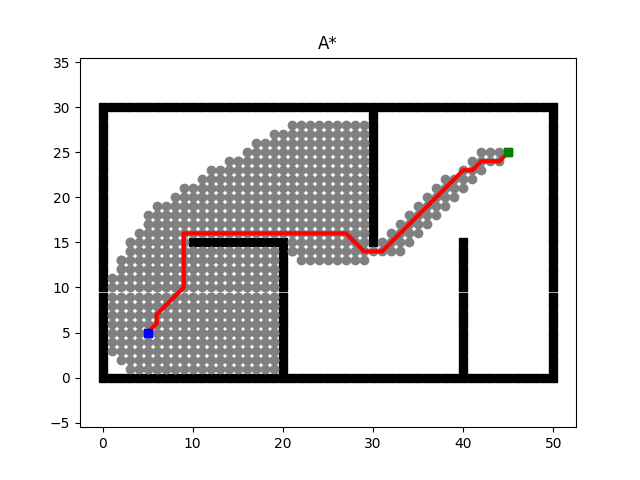
\includegraphics[width=0.4\textwidth]{fig/插图/A-search/Astar.png}}
			\subcaptionbox{Dijstra\label{fig:Dijstra}}[0.49\textwidth]{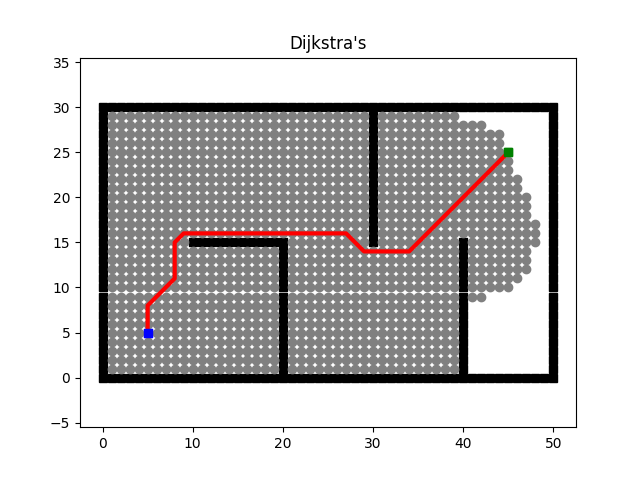
\includegraphics[width=0.4\textwidth]{fig/插图/A-search/Dijstra.png}}
			\subcaptionbox{ARAstar\label{fig:ARAstar}}[0.49\textwidth]{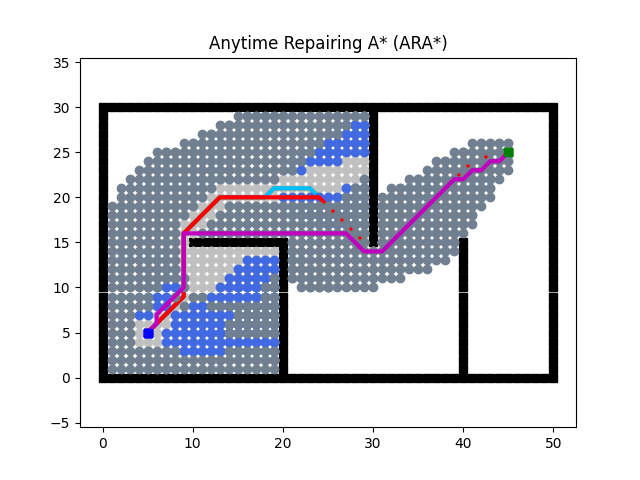
\includegraphics[width=0.4\textwidth]{fig/插图/A-search/ARAstar.png}}
			\subcaptionbox{LPAstar\label{fig:LPAstar}}[0.49\textwidth]{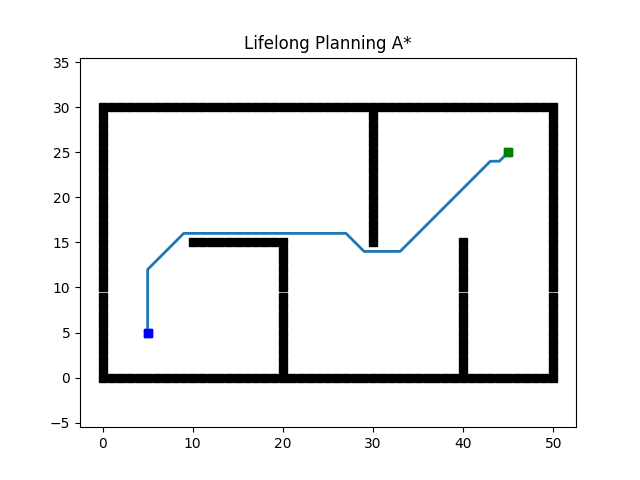
\includegraphics[width=0.4\textwidth]{fig/插图/A-search/LPAstar.png}}
			\subcaptionbox{RTAAstar\label{fig:RTAAstar}}[0.49\textwidth]{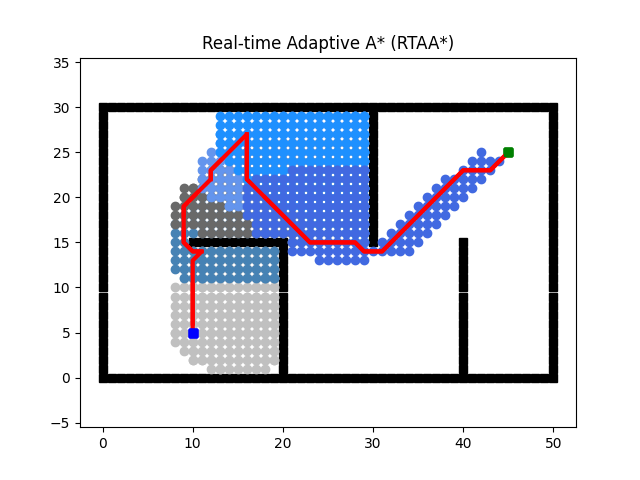
\includegraphics[width=0.4\textwidth]{fig/插图/A-search/RTAAstar.png}}
			\subcaptionbox{Dstar\label{fig:Dstar}}[0.49\textwidth]{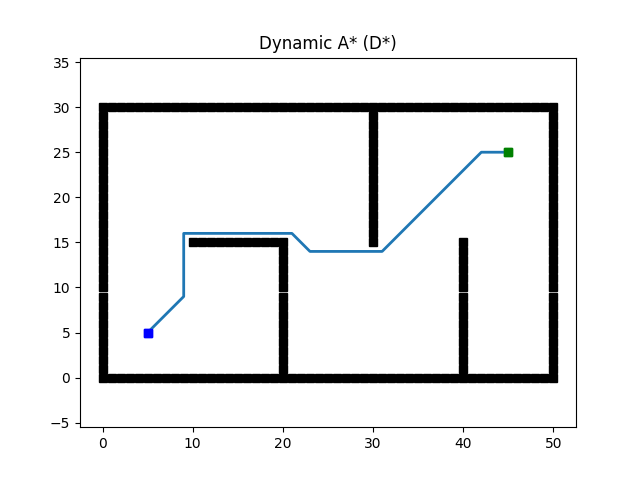
\includegraphics[width=0.4\textwidth]{fig/插图/A-search/Dstar.png}}
			\caption{基于搜索的路径规划算法效果对比图}
			\label{fig:基于搜索的路径规划}
		\end{figure}
		Dijkstra算法\upcite{Dijstra1959}作为图论经典算法,通过广度优先搜索首次系统解决了带权重图的最短路径问题,但其盲目性导致时间复杂度随环境规模呈指数级增长,难以满足实时规划需求。A*算法\upcite{hart1968formal}创新性地引入启发式函数,将搜索方向聚焦于目标区域,在保证路径最优性的同时显著降低计算复杂度,奠定了启发式搜索的理论基础。然而,该算法仍存在两大局限:其一,内存消耗随搜索空间扩大呈指数级增长;其二,启发函数依赖先验环境知识,难以适应动态障碍物或未知地形。D*算法\upcite{stentz1994optimal}采用反向搜索机制与增量更新策略,仅在环境变化时局部修正路径,将重规划时间复杂度从从$O(n^2)$降至$O(k)$,使机器人能在未知地形中实时避障。但其路径振荡现象仍会影响轨迹平滑性,且在复杂动态场景中频繁更新易导致累积误差累积。Koenig等人\upcite{koenig2004lifelong}提出的LPA*(Lifelong Planning A*)通过维护优先队列的键值一致性,实现历史搜索信息的智能复用,使得连续规划场景的搜索速度大幅度提升,但其内存管理机制仍无法有效应对长期运行中的状态爆炸问题。Likhachev团队\upcite{likhachev2003ara}提出ARA*(Anytime Repairing A*)算法引入次优性容忍系数,允许算法在有限时间内输出渐进优化的路径,为无人机紧急避障等实时性要求严苛的场景提供了解决方案,但路径质量与计算资源的平衡仍需人工调参。

		LRTA*(Learning in real-time A*)算法\upcite{bulitko2006learning}通过动态调整搜索深度和智能剪枝策略,将启发式搜索延迟控制在毫秒级,但其剪枝机制可能丢失潜在最优路径分支。JPS算法\upcite{harabor2011online}针对栅格地图提出“跳跃点”,通过识别路径对称性跳过大量无效节点,在保持最优性的前提下将搜索速度提升10倍以上,但该方法仅适用于均匀网格环境,且无法处理动态障碍物。RTAA*(Real-time adaptive A*)算法\upcite{koenig2006real}结合在线学习机制,利用实际移动代价动态更新启发函数,使智能体在未知地形中的路径收敛速度得到提升,但其依赖大量交互数据的学习过程在稀疏奖励场景中表现受限。

		
		

		\subsection{基于采样的运动规划方法}
		基于采样的路径规划方法通过在地图中随机生成采样点来探索可能的路径。这些采样点被生成在整个可行空间内,任何落在障碍物区域内的点都会被排除在外。剩余的采样点随后被相互连接,形成一条从起点到终点的路径。与基于搜索图结构的传统方法不同,基于采样的方法特别适合解决高维空间中的路径规划问题,因为它们不需要对整个空间进行详尽的离散化。这类采样的算法在理论上具有概率完备性,这意味着只要存在一个解,在足够长的时间内,通过不断采样,算法几乎可以确定地找到至少一个可行解。这种特性使得基于采样的路径规划方法在处理复杂和动态环境时显得尤为有效。此外,随着计算时间的增加,找到最优或接近最优解的概率也会相应提高。图\ref{fig:基于采样的路径规划}是几种RRT系列采样规划算法的仿真效果图。
		\begin{figure}[H]
			\centering
			\subcaptionbox{RRT\label{fig:RRT}}[0.49\textwidth]{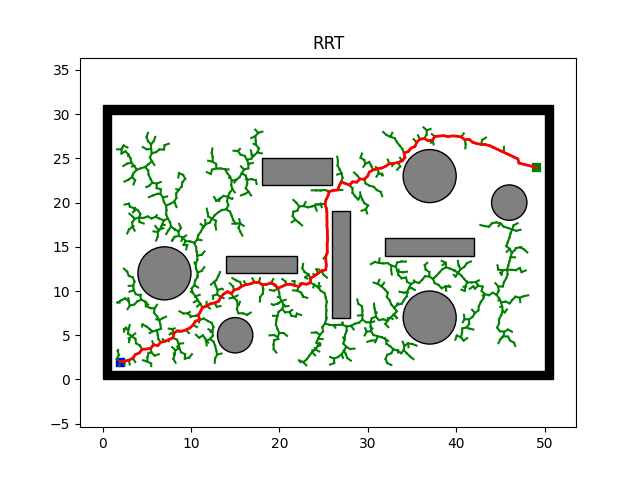
\includegraphics[width=0.4\textwidth]{fig/插图/rrt/RRT.png}}
			\subcaptionbox{RRT Connect\label{fig:RRT_connect}}[0.49\textwidth]{\includegraphics[width=0.4\textwidth]{fig/插图/rrt/RRT\_connect.png}}
			\subcaptionbox{Informed RRTstar\label{fig:informed_RRTstar}}[0.49\textwidth]{\includegraphics[width=0.4\textwidth]{fig/插图/rrt/informed\_RRTstar.png}}
			\subcaptionbox{Fast Matching Trees\label{fig:fast_matching_trees}}[0.49\textwidth]{\includegraphics[width=0.4\textwidth]{fig/插图/rrt/fast\_matching\_trees.png}}
			\subcaptionbox{Extended RRT\label{fig:extended_RRT}}[0.49\textwidth]{\includegraphics[width=0.4\textwidth]{fig/插图/rrt/extended\_RRT.png}}
			\subcaptionbox{Batch Informed Trees\label{fig:batch_informed_trees}}[0.49\textwidth]{\includegraphics[width=0.4\textwidth]{fig/插图/rrt/batch\_informed\_trees.png}}
			\caption{基于采样的路径规划效果对比图}
			\label{fig:基于采样的路径规划}
		\end{figure}


		RRT(Rapidly-exploring Random Trees)算法\upcite{lavalle2001rapidly}开创性地结合了随机采样与树形结构,通过倾向于未探索区域的生长策略,有效应对高维构型空间和非完整约束问题。其概率完备性的特性为后续的采样算法奠定了理论基础,但该算法生成路径的质量并不保证最优。为了提高查询效率,RRT-Connect算法\upcite{kuffner2000rrt}引入双向树增长与贪心连接策略,显著加快了在复杂环境中的收敛速度,成为实时机器人导航的关键技术之一。然而,这类算法主要集中在寻找可行解,未能解决路径最优性的问题。
		针对动态环境下的实时规划需求,ERRT(Execution-extended RRT)算法\upcite{bruce2002real}通过引入路径点缓存和自适应成本惩罚机制,在重规划中复用历史路径信息,解决了传统RRT在动态障碍物场景下重复计算的问题,实现了首次实时在线规划。尽管如此,ERRT的路径优化依赖于启发式规则,缺乏全局最优性保障。
		进一步的发展包括RRT*算法\upcite{karaman2011sampling},它不仅能够在复杂环境中高效找到可行路径,还能优化路径以达到时间或距离上的最优,特别是在高维空间中表现优异。Informed RRT算法\upcite{6942976}则通过椭圆启发式采样,将搜索限制在可能改进当前解的区域内,提升了收敛速度和最终路径质量,并首次从理论上证明了采样算法可渐进趋近最优解。这揭示了传统RRT因全局均匀采样导致的效率瓶颈,为后续最优性导向算法提供了理论依据。
		最后,BIT*(Batch Informed Trees)算法\upcite{7139620}融合了图搜索(基于A*启发式)与批处理采样的方法,在隐式随机几何图上执行增量搜索,解决了高维空间中传统算法收敛缓慢的问题。这些进展标志着从单纯追求“可行解”向确保“最优解”的转变,但在面对高维场景时,仍需克服计算复杂度极高的困难。

		\subsection{基于曲线插值的运动规划方法}
		基于曲线插值的运动规划方法以其路径平滑性的显著优势,区别于图搜索和采样规划方法。图\ref{fig:基于曲线插值的路径规划}展示了多种曲线插值算法的效果。
		早期的研究主要集中在静态环境下的几何路径求解,Reeds-Shepp曲线\upcite{reeds1990optimal}作为这一领域的先驱,为车辆运动规划奠定了理论基础。它在Dubins曲线\upcite{gupta2022shortest}的基础上引入倒车机制,证明了包含至多两个尖点的CCSCC型路径(圆-圆-直线-圆-圆)即可构成最优解。通过构建48种候选路径形式,解决了双向行驶车辆在最小转弯半径约束下的最短路径问题。然而,该方法局限于二维平面几何推导,并未考虑动态障碍物和实时计算需求,在复杂场景下其枚举式搜索效率较低。
		随着自动驾驶技术的发展,百度Apollo团队于2017年提出的EM Motion Planner算法\upcite{fan2018baidu}标志着向动态环境适应性和多约束协同优化的重大进步。该系统采用Frenet坐标系下的路径-速度迭代优化,结合动态规划粗搜索与二次规划细优化,实现了交通规则、障碍物决策与运动平滑性的多目标协同。其创新之处在于将决策问题转化为可行轨迹生成,通过构建凸可行空间确保了解的存在性。
		Gao等人\upcite{Gao2018OnlineST}利用安全飞行走廊和贝塞尔曲线\upcite{lee2021optimal}提出了一种优化方法以构建时间最优轨迹,推动了无人机领域实时规划的发展。该方法巧妙地结合快速行进法与ESDF(截断符号距离场),构建速度自适应的时空索引路径,解决了传统方法中时间分配不合理的问题。通过利用贝塞尔曲线的凸包特性,首次实现了轨迹整体安全性和高阶动力学约束的严格保证。仿真结果表明,该方法能够在未知环境中实时生成安全轨迹,但在狭窄空间中的飞行走廊膨胀策略可能过于保守,且未能有效处理动态障碍物的预测与避让。
		\begin{figure}[H]
			\centering
			\subcaptionbox{Bezier Curve\label{fig:bezier}}[0.49\textwidth]{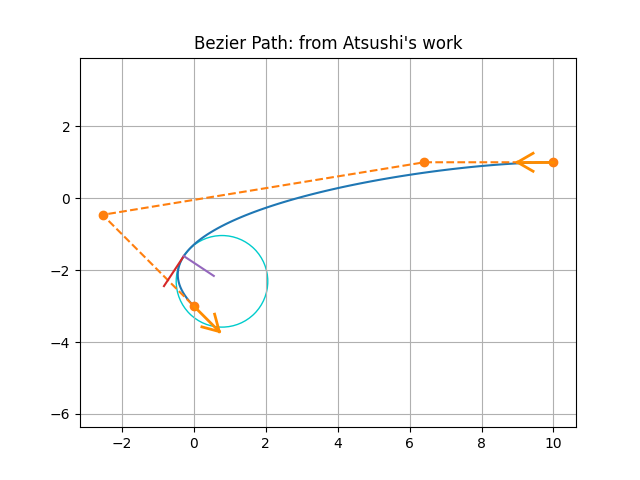
\includegraphics[width=0.4\textwidth]{fig/插图/curve/bezier.png}}
			\subcaptionbox{Bspline\label{fig:bspline}}[0.49\textwidth]{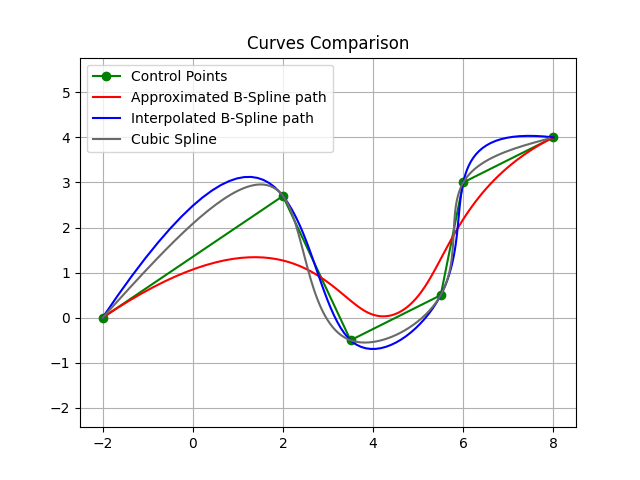
\includegraphics[width=0.4\textwidth]{fig/插图/curve/bspline.png}}
			\subcaptionbox{Dubins Curve\label{fig:dubins_path}}[0.49\textwidth]{\includegraphics[width=0.4\textwidth]{fig/插图/curve/dubins\_path.png}}
			\subcaptionbox{Reeds Shepp Curve\label{fig:reeds_shepp}}[0.49\textwidth]{\includegraphics[width=0.4\textwidth]{fig/插图/curve/reeds\_shepp.png}}
			\caption{基于曲线插值的路径规划效果对比图}
			\label{fig:基于曲线插值的路径规划}
		\end{figure}
		
		Nguyen团队\upcite{10160561}提出了多面体导航工具箱,将路径规划抽象为凸多面体序列内的B样条优化问题。通过将B样条转换为等效贝塞尔表示,显著提升了局部凸性约束的紧密度,使得线性约束控制点即可保障全局安全性。该工作建立了从栅格地图到多面体地图的完整流程,支持最小控制点、代数解等多种优化模式。然而,多面体序列的构建依赖静态环境假设,在动态场景中需要频繁重规划,且高维凸优化问题的实时性仍有待提升。
		

		\subsection{基于优化的运动规划方法}
		Li等\upcite{li2015unified}提出了一种基于时间最优控制(Optimal Control)的动态优化框架,该框架将平行、垂直等规则停车场景与不规则障碍物场景统一建模。通过严格描述车辆运动学、机械约束及碰撞条件,并采用内点法求解非线性优化问题,该方法构建了一个开放框架,允许用户自定义约束和优化目标。然而,由于其计算复杂度较高,难以满足实时性需求。
		Kondak等\upcite{933030}则将路径规划转化为非线性最优控制问题,利用序列二次规划(SQP)直接优化轨迹,并引入人工势场来处理障碍物碰撞,支持全维车辆模型。尽管这种方法在处理障碍物时表现出一定的灵活性,但其势场函数设计依赖于经验参数,且未解决非凸优化对初值敏感的问题。
		Arantes等\upcite{8613017}针对离散时间步间的“跳跃碰撞”问题,提出了基于混合整数线性规划(MILP)的连续时间碰撞避免编码方法。通过确保相邻状态位于障碍物同侧,保证了轨迹段的安全性,并引入机会约束至风险分配框架,平衡了路径的安全性和保守性。虽然该方法显著提升了非凸环境下的路径安全性,但由于MILP的NP-hard特性,限制了其在大规模障碍物场景中的应用扩展性。
		Zhang与Borrelli等\upcite{9062306}提出的OBCA(Optimization-Based Collision Avoidance)框架进一步创新,通过强对偶定理重构平滑碰撞约束,将非凸避障条件转化为可微优化问题,支持全维物体与复杂障碍物。符号距离函数用于量化侵入程度,实现了“最小侵入”轨迹生成。然而,此方法要求障碍物分解为凸集,导致预处理成本较高。
		Zhang等\upcite{8619433}提出的分层优化框架H-OBCA(Hierarchical-OBCA),结合了Hybrid A算法\upcite{chang2024hybrid}的全局搜索能力与优化碰撞避免(OBCA)的局部精细化调整。Hybrid A基于简化模型快速生成粗路径,OBCA则利用全维模型优化路径的平滑性和动态可行性,解决了非凸优化依赖初值的瓶颈。实验表明,该方法在狭窄场景中能够实现实时规划,且生成的轨迹可以被底层控制器精准跟踪。然而,其性能受限于Hybrid A*的路径质量,在复杂障碍布局下可能陷入局部最优。

	\section{铰接车运动规划技术国内外研究现状}
	铰接车路径规划的研究历程可追溯至2010年代初期的几何建模与静态环境规划阶段。图\ref{fig:几种典型的铰接车案例}为几种常见的铰接车类型。早期的代表性工作如Choi与Huhtala提出基于Bezier曲线的分层规划框架\upcite{choi2015constrained},其核心贡献在于将参数化曲线与搜索算法结合,通过离线生成满足非完整约束的运动基元库(包含曲率连续的前进/倒车路径片段),再结合A*算法在线搜索全局路径,并引入非线性优化修正关节角度超限问题。Sarata等人\upcite{yossawee2002path}针对轮式装载机的V型作业路径提出对称Clothoid曲线连接策略,通过数学证明得出Clothoid曲线的曲率线性变化特性可消除传统线-弧路径的曲率突变问题,但其固定路径模式依赖预设的装载点与卸载点位置,难以适应砂石堆形状动态变化的非结构化场景。 Nayl等\upcite{nayl2013line}将模型预测控制(MPC)与Bug算法结合,提出基于铰接车误差动力学模型的滚动优化框架,通过实时调整前轮转向角与车速实现动态避障。该方法在仿真中成功处理了突然出现的移动障碍物,路径跟踪误差控制在±0.15m以内,但未解决多周期任务的长时优化问题,且在狭窄通道中易因局部最优陷入死锁。Chen等\upcite{9216948}对比了简化单车模型与双体铰接模型的规划效果,发现复杂模型在双向倒车场景中可生成更短的安全路径,但计算耗时增加,揭示了模型精度与实时性之间的固有矛盾。Hong团队\upcite{8500447}进一步引入3D地形高程数据构建动力约束,提出动态规划(DP)与MPC结合的混合方法,在轮式装载机的崎岖地形实验中实现能耗降低,但其离散化状态变量导致高维空间下的计算复杂度呈指数级增长,难以扩展至多关节车辆。Kawabe等\upcite{Kawabe02122021}设计的分级优化框架将全局任务分解为铲取点选择、卸载点规划与局部路径生成子问题,并首次引入深度强化学习(DRL)实现动态砂石堆的自适应装载路径规划。
	\begin{figure}[H]
		\centering
		\subcaptionbox{轮式装载机\label{fig:loader_real}}[0.49\textwidth]{\includegraphics[width=0.4\textwidth]{fig/插图/loader\_real.png}}
		\subcaptionbox{四驱铰接式叉车\label{fig:四驱铰接式叉车}}[0.49\textwidth]{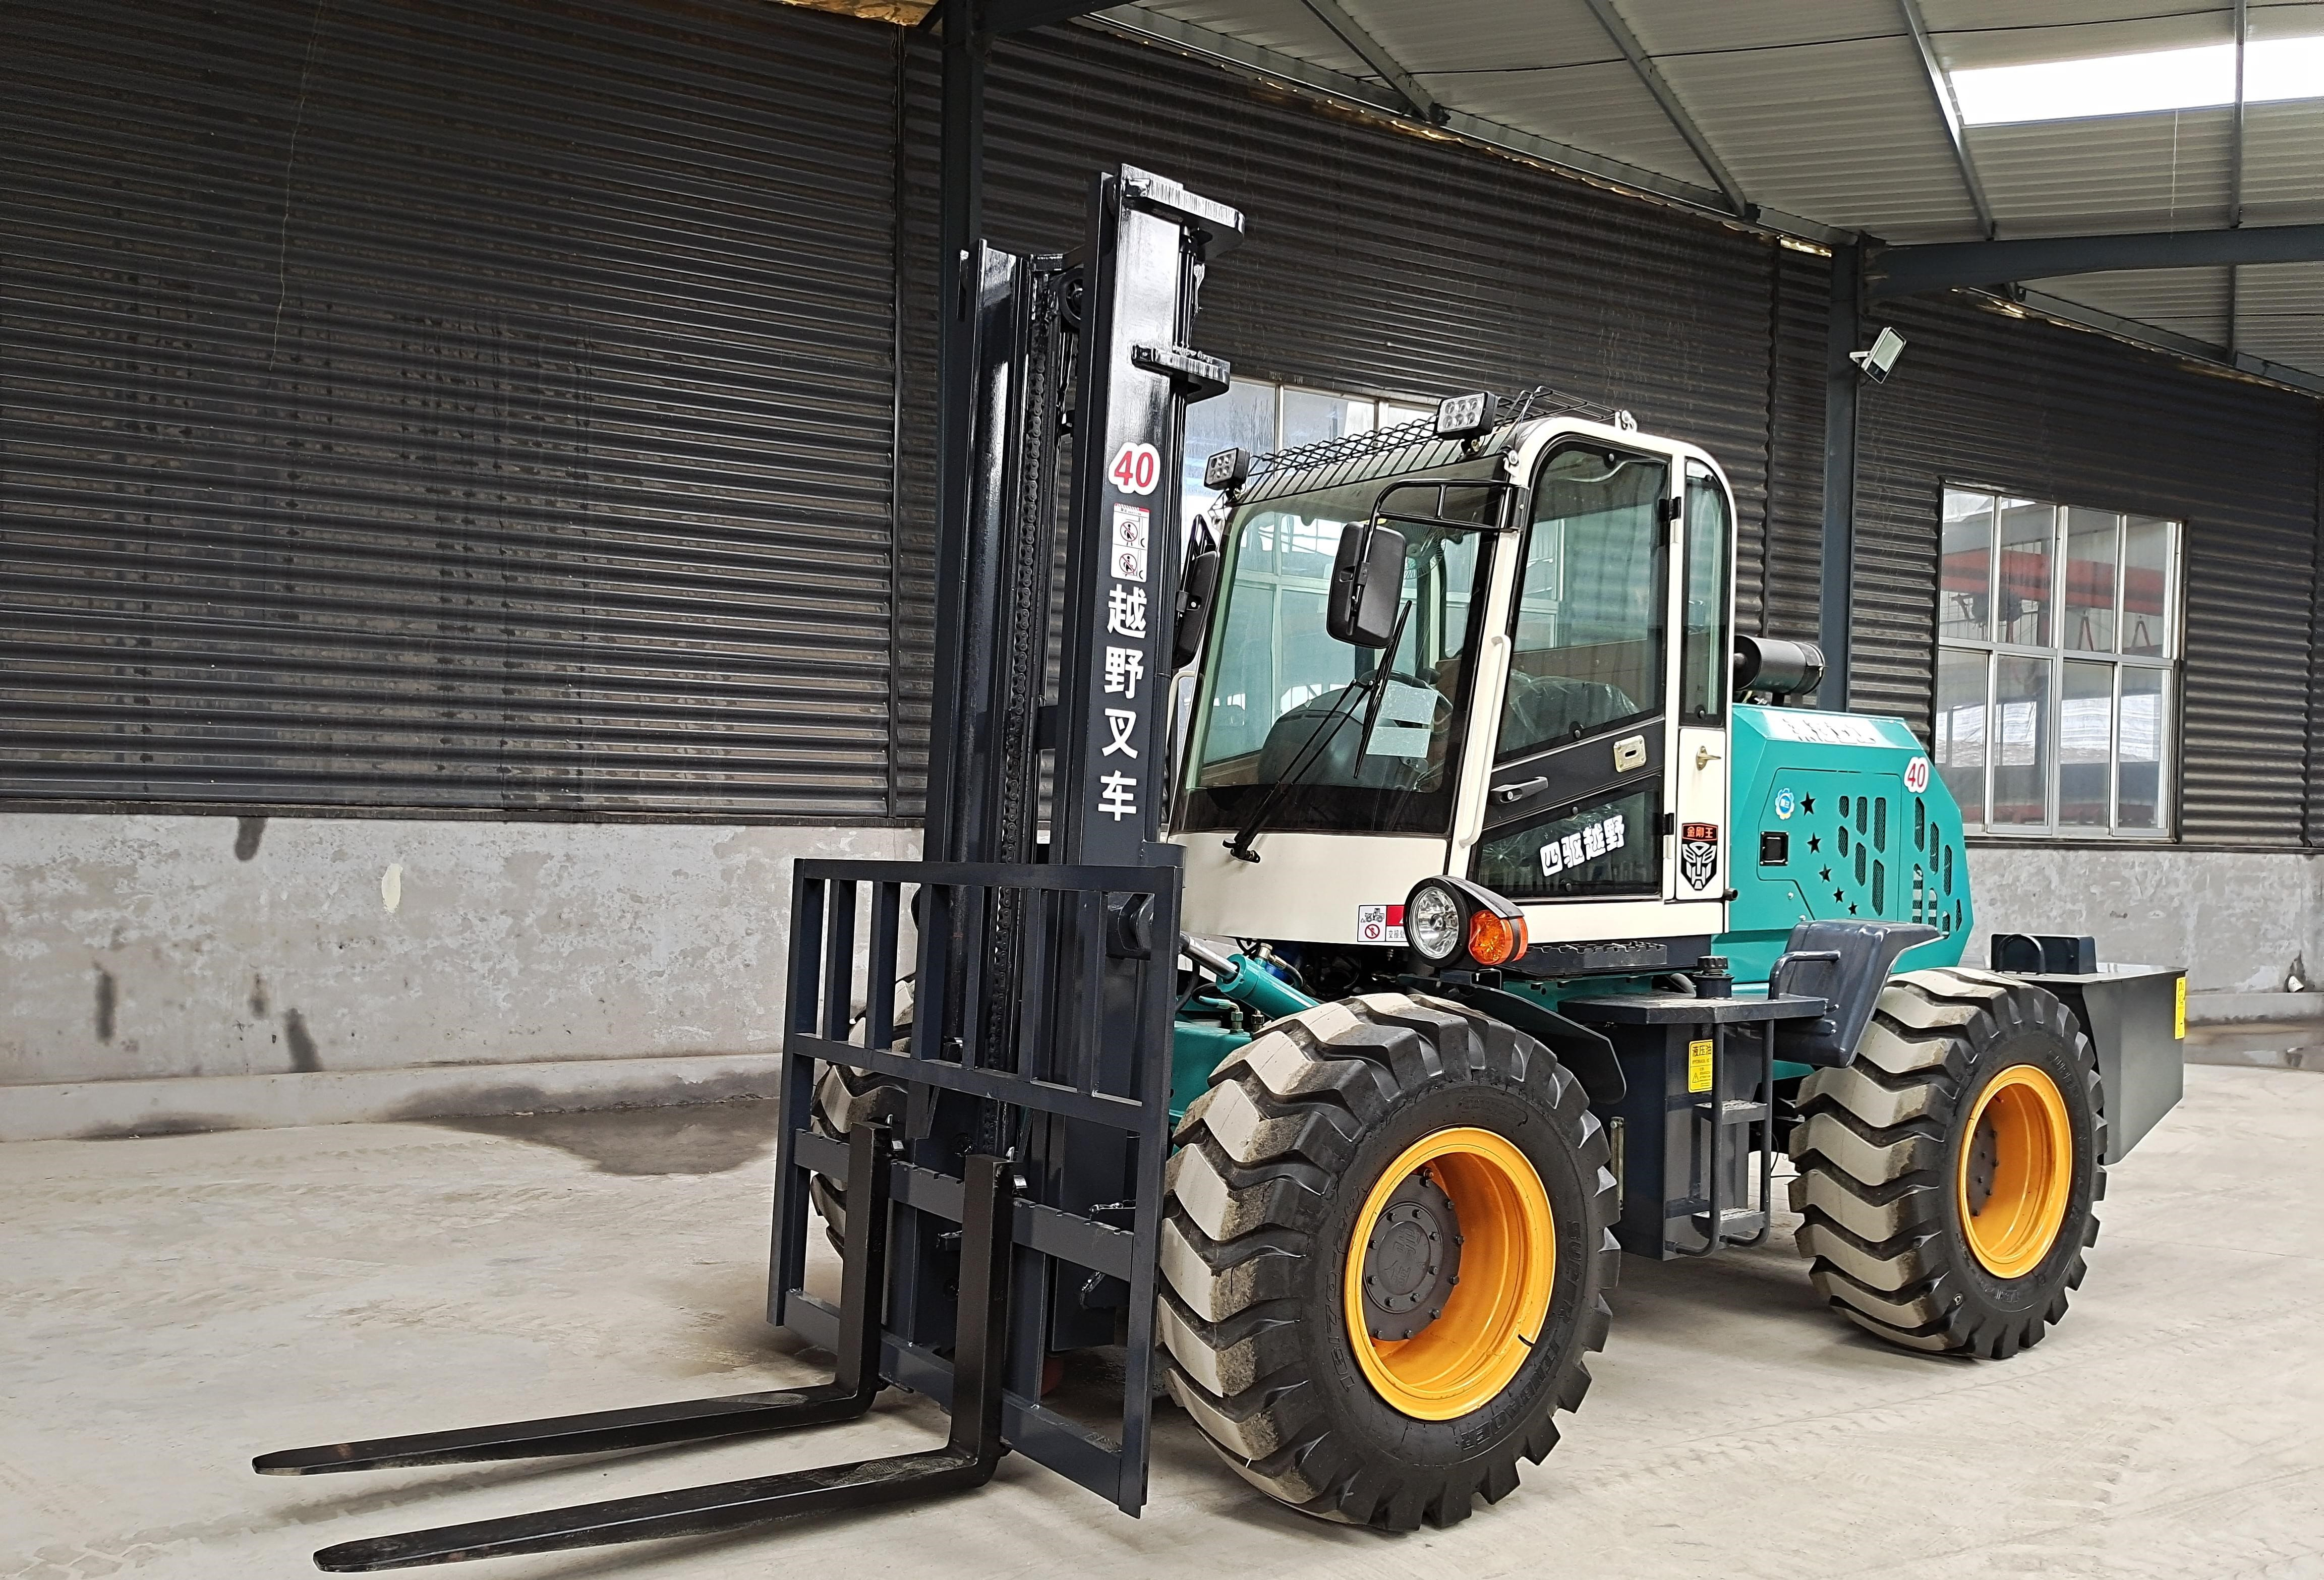
\includegraphics[width=0.4\textwidth]{fig/插图/四驱铰接式叉车.jpg}}
		\subcaptionbox{沃尔沃A30F铰接式卡车\label{fig:沃尔沃A30F铰接式卡车}}[0.49\textwidth]{\includegraphics[width=0.4\textwidth]{fig/插图/沃尔沃A30F铰接式卡车.png}}
		\subcaptionbox{沃尔沃A35F铰接式卡车\label{fig:沃尔沃A35F铰接式卡车}}[0.49\textwidth]{\includegraphics[width=0.4\textwidth]{fig/插图/沃尔沃A35F铰接式卡车.png}}
		\caption{几种常见的铰接车:铰接式叉车、轮式装载机、铰接式四驱卡车}
		\label{fig:几种典型的铰接车案例}
	\end{figure}
	
	Zhao等\upcite{zhao2022time}采用Chebyshev伪谱法对重型铰接车垂直泊车问题进行时间最优轨迹优化,通过精确建模非完整约束,使得求解的精度大幅提高。Shi等\upcite{shi2020planning}提出的自适应MPC跟踪系统通过曲率扰动补偿机制,在非均匀路面下将路径跟踪的横向位移误差有所降低,但其依赖RTK-GPS的高精度定位信号,在卫星遮挡的室内仓储场景中性能显著下降。
	
	基于优化的运动规划算法,尤其是模型预测在近期一直是研究的热点,原因在于其相较于基于搜索和采样的规划方法,能够求解出更加圆滑且满足各种约束的轨迹\upcite{孟宇2019基于预瞄距离的地下矿用铰接车路径跟踪预测控制,贾生超2023牵引挂车垂直泊车路径规划与运动控制,杜青炎2023基于改进混合}。其缺点是在大量约束的情况下求解会变得很困难。但是在当下计算机高速发展,优化问题的求解时间逐渐不再是问题的瓶颈。所以基于优化的轨迹规划方法是很值得研究的方向之一。

	\section{本文研究的主要内容}
	本研究针对铰接车辆在复杂非结构化环境中的轨迹规划问题,采用全局与局部规划相结合的方法,旨在解决传统算法因忽略铰接车强非完整性与运动学约束导致的路径不可跟踪、避障安全性不足等问题。

	本课题的研究内容和解决的关键问题如下:

	(1)基于微分平坦全局轨迹规划方法。

	首先,将微分平坦理论引入铰接车轨迹规划,通过平坦变量的多阶导数表示系统输入和状态变量,简化规划问题并增强数值稳定性。其次,将车辆前桥与后桥建模为双凸结构,采用安全走廊表征避障安全性。此外,建立基于Minco样条(Minimum Control Effort Spline)的轨迹优化模型,将高维优化问题转换为低维避障优化问题。最后,设计曲率约束松弛函数,将路径规划转化为无约束优化问题,并采用L-BFGS(Limited-memory Broyden–Fletcher–Goldfarb–Shanno Algorithm)算法实现高效求解,确保轨迹满足转向半径与避障要求。

	(2)基于NMPC和安全走廊的局部轨迹规划研究。

	首先,构建非线性模型预测控制(NMPC, Nonlinear Model Predictive Control)框架描述轨迹规划问题。其次,引入安全走廊策略保障轨迹安全性,研究走廊约束重构方法以降低求解难度。最后,设计外罚函数策略与微分同胚变换,在保持问题凸性的前提下实现无约束优化转换,提升求解效率,规避高维优化变量导致的维度灾难。

	\section{本文结构安排}
	本文各章节的结构与内容如下:

	第一章:绪论。本章阐述铰接车在复杂环境(如港口、矿山)中的运动规划研究背景与意义,分析非完整约束带来的轨迹规划挑战。系统梳理国内外运动规划技术的研究现状,涵盖基于图搜索、采样、曲线插值与优化的方法,以及铰接车专用算法的进展与局限性。明确本文研究目标与创新点,提出融合全局与局部规划的优化框架,并概述全文结构。

	第二章:铰接车运动学模型与规划系统设计。本章构建铰接车轨迹规划的数学模型,推导其运动学方程与转弯半径。将规划任务分为全局和局部两部分,基于最优控制理论对规划问题进行建模。阐述问题的求解方法,并将其离散化为非线性规划(NLP)形式。

	第三章:铰接车微分平坦全局轨迹规划。基于铰接车微分平坦特性,采用Minco样条参数化轨迹,结合RRT-Connect生成初始路径。设计凸多边形安全走廊约束,通过松弛函数处理曲率与避障条件,利用L-BFGS算法实现高效优化。针对多阶段任务(如码头装卸),提出换向点处理机制,并通过仿真验证算法在复杂场景的有效性。

	第四章:基于安全走廊的局部轨迹规划。针对传统Hybrid A*算法不适应铰接车的问题,提出改进方法并用于算法的热启动。构建基于安全走廊的NMPC框架,以舒适性、能耗与时间为优化目标,集成Bresenham栅格检测算法与高阶运动学约束,通过IPOPT求解器实现动态避障与实时优化。

	第五章:运动规划系统仿真验证。基于ROS机器人系统和RVIZ仿真软件搭建仿真平台。设计包含障碍物规避、泊车、侧边停车、狭窄空间穿行及对向掉头等场景,分别验证全局与局部规划算法的可行性。

	第六章:总结与展望。本章总结研究内容与成果,分析创新点。讨论现存问题,提出未来研究方向。

	\chapter{基于最优控制的铰接车运动规划问题建模}
	\section{铰接车运动学模型建立}
	铰接车结构上由前桥和后桥组成,中间通过液压或者舵机驱动铰接角完成转向。本文介绍的铰接车结构模型如图\ref{fig:铰接车简易模型}所示。 
	\begin{figure}[H]
		\centering
		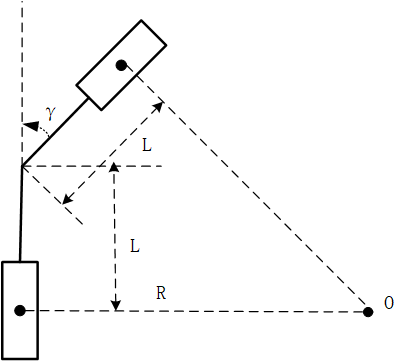
\includegraphics[width=0.6\textwidth]{铰接车简易模型.png}
		\caption{铰接车简易模型}
		\label{fig:铰接车简易模型}
	\end{figure}

	图中,前轴中点$P(x,y)$为前轴中点位置,$P_r(x_r,y_t)$为后轴中点位置。也是整车参考点。$\theta$为前轴的航向角,$\theta_r$为后轴航向角。$O$点为瞬时转向圆心,o1为铰接点。$l_f$是前轴长度,$l_r$是后轴长度,$\gamma$是铰接角,$R$为车体转弯半径。考虑到铰接车工作在小范围场景,做出两个假设:(1)铰接车辆始终保持低速运动,忽略动力学特性。(2)假设车辆不发生侧滑。
	由于车辆不会发生打滑,所以车辆运动时前后车轮完全满足车辆的滚动约束,即速度方向和车辆的朝向保持一致,从而可以得到:
	\begin{equation}
		\begin{aligned}
			&\dot{x}=v\cos\theta\\
			&\dot{y}=v\sin\theta\\
			&\dot{x}\sin\theta-\dot{y}\cos\theta=0\\
			&\dot{x}_r\sin\theta _r-\dot{y}_r\cos\theta _r=0
		\end{aligned}
		\label{model_1}
	\end{equation}
	其中,$v$为车体前桥的参考点速度,$\dot{x}$和$\dot{y}$分别为铰接车位置$x$和$y$对时间的导数。

	由于前桥和后桥通过铰接角刚性连接,可以推导出前桥参考点和后桥参考点的坐标变换见式(\ref{model_2}):
	\begin{equation}
		\begin{aligned}
			&x=x_r+l_r\cos\theta _r+l_f\cos\theta\\
			&y=y_r+l_r\sin\theta _r+l_f\sin\theta\\
			&\theta _r=\theta-\gamma 
		\end{aligned}
		\label{model_2}
	\end{equation}

	在本文的研究中铰接车的前桥和后桥相等,即$L=l_f=l_r$。联合式(\ref{model_1})和式(\ref{model_2})可以得到铰接车的运动学模型,见式(\ref{eq:铰接车运动学模型})。
	\begin{equation}
		\begin{aligned}
			\frac{\mathrm{d}}{\mathrm{d}t}\left[ \begin{array}{c}
				x\\
				y\\
				\theta\\
				\gamma\\
			\end{array} \right] =\left[ \begin{array}{c}
				v\cos\theta\\
				v\sin\theta\\
				v\tan( \gamma /2 ) /L+\omega /( \cos\gamma +1 )\\
				\omega\\
			\end{array} \right] 
		\end{aligned}
		\label{eq:铰接车运动学模型}
	\end{equation}
	其中,$v,\omega$是输入量,分别代表这前轴速度和铰接角速度。详细的运动学模型推导过程可以参考文献\cite{corke2001steering}。

	接着可以推导出铰接车的转弯半径为:
	\begin{equation}
		\begin{aligned}
			R = \frac{v}{\dot{\theta}} = v\cdot L \frac{1+\cos\gamma}{v\sin\gamma+L\omega }
		\end{aligned}
		\label{eq:转弯半径}
	\end{equation}


	特别的,如果忽略铰接车的动态转向,只保留静态转向,即$\omega=0$,式(\ref{eq:转弯半径})可以重写为:
	\begin{equation}
		\begin{aligned}
			R_{steady} = \frac{L}{\tan(\gamma/2)} 
		\end{aligned}
	\end{equation}
		
	\section{基于最优控制的运动规划问题建模}
	本文设计的全局和局部规划器都使用了基于优化的方法,将问题构建在最优控制的框架下求解。最优控制的一大特点就是可以清晰的把各种约束表示在问题里,例如运动学方程约束、状态受限约束和执行器受限约束\upcite{刘凯2018高速无人驾驶车辆最优运动规划与控制的动力学建模分析}。
	
	假设系统状态方程为$\dot{x}(t)=f(x(t),u(t))$,最优控制就是从可选择的容许控制集$U$中,找到一个控制矢量$u(t)$,使得系统到终端时刻时,性能代价取最小值,此刻满足条件的控制称为最优控制$u^{*}(t)$,对应的状态方程的解成为最优轨线$x^{*}(t)$。最优控制侧重于得到系统的最优控制量,轨迹规划与之不同,它侧重于得到系统的状态量,即最优轨线。
	
	轨迹规划在最优控制的表述下属于代价函数是综合型或鲍尔扎型的性能指标,它通常包括能量消耗和终点代价两个部分\upcite{anderson2010optimal}。基于连续系统的鲍尔扎型最优控制可以将轨迹规划表述为:
	\begin{equation}
		\begin{aligned}
			\min_{x(t),u(t),t} &J = \Phi[x(t_f)]+\int_{t_0}^{t_f}L[x(t),u(t),t]dt\\
			s.t. \ \ \ &\dot{x} = f(x(t),u(t))\\
			&x_{min}\le x(t) \le x_{max},u_{min}\le u(t) \le u_{max},t \in{t_0,t_f}\\
			&x(t_0)=x_{start},x(t_f)=x_{goal}\\
			&h(x(t))\cap C_{occ}=\varnothing 
		\end{aligned}
	\end{equation}
	其中,$\Phi[x(t_f)]$为终点$x(t_f)$的代价,$L[x(t),u(t),t]$为时间$t$时刻的过程代价。$\dot{x}(t)=f(x(t),u(t))$为车辆的运动学方程,$x_{min}$和$x_{max}$分别为状态变量的下边界和上边界。$u_{min}$和$u_{max}$分别为输入变量的下边界和上边界。$x(t_0)=x_{start},x(t_f)=x_{goal}$表示起点和终点约束。$h(x(t))\cap C_{occ}=\varnothing$表示车辆的避障约束,其中$C_{occ}$表示障碍物区域。
	
	对于离散系统,一般代价泛函可以表示为:
	\begin{equation}
		\begin{aligned}
			J = \Phi[x(N)]+\sum_{k=k_0}^{N-1}L[x(k),u(k),k]
		\end{aligned}
	\end{equation}
	其中,$\Phi[x(N)]$为终点$x(N)$的代价函数,$L[x(k),u(k),k]$为第$k$步的过程代价函数。$x(k)$和$u(k)$表示第$k$步的状态量和控制量,$N$是控制区间长度,$J$是最优控制的目标函数。

	\section{最优控制问题的解法}
	最优控制问题的求解方法主要可分为两类。一类是解析解法,基于变分法原理与极小值原理的经典分析方法\upcite{彭海军2011求解最优控制问题的混合变量变分方法及其航天控制应用}。这类方法通过严格的数学推导获得控制律的显式解析解,具有理论完备性强的特点。然而其应用受限于问题复杂度,当系统动力学方程非线性程度加剧或路径约束增多时,解析解的推导将面临难以逾越的数学障碍,导致方法失效。另一类是数值解法,采用离散化策略将连续最优控制问题转化为非线性规划问题求解。此类方法虽能处理复杂约束条件与非线性系统,但随着精度要求的提升(包括时间离散密度与状态量精度),会导致优化变量维度呈指数级增长。由此产生的计算复杂度将显著延长求解时间,严重影响控制系统的实时性表现。这两类方法呈现不同的特性,解析解法在简单场景中具有理论优势却缺乏工程适用性。而数值解法具广泛适应性但受制于“维度灾难”带来的计算瓶颈。本文使用数值解法,因为后续提出的策略可以有效解决高维度下求解难的问题。
	\subsection{极小值原理}
	作为最优控制理论的基石之一,庞特里亚金于1956年建立的极小值原理\upcite{mehta2009q}突破了经典变分法的约束条件限制。该原理通过引入协态变量构建哈密顿函数体系,在容许控制域内寻找使哈密顿函数极小的最优控制序列。其核心在于求解如下微分方程系统:
	\begin{equation}
		\begin{cases}
		\dot{x} = \frac{\partial H}{\partial \lambda} \\
		\dot{\lambda} = -\frac{\partial H}{\partial x} \\
		H(x^*,u^*,\lambda^*,t) = \min_{u \in \Omega} H(x^*,u,\lambda^*,t) 
		\end{cases}
	\end{equation}
	其中,$x$为状态变量,$u$为容许控制输入,$\lambda$为协态变量,哈密顿函数$H(x,u,\lambda,t)=L(x,u,t)+\lambda f(x,u,t)$由性能指标中的被积函数$L$和状态方程函数$f$共同构成。
	相较于传统变分法,其创新在于允许控制变量存在闭集约束,并能有效处理终端状态受限的边值问题。在工程实践中,该原理为航天器轨道转移、机器人轨迹规划等典型最优控制问题提供了严格的判据。然而,在强非线性系统中,协态方程与状态方程的强耦合常导致两点边值问题的解析不可解,这一挑战推动了数值求解算法的发展,通过离散化将连续最优控制问题转化为非线性规划问题求解。
	
	\subsection{基于配点法的数值求解}
	配点法通过离散控制量和状态量将连续最优控制问题转化为非线性规划问题(nonlinear programming problem, NLP),其数值鲁棒性在工程领域广受认可\upcite{aluru2000point}。由于直接将状态量纳入到优化变量,得到的最优解就是所求轨迹,所以配点法适合用来做轨迹规划。这种方法在配点处要求满足动力学方程约束,配点之间使用多项式或者其他曲线进行插值。当配点较为密集时,配点之间也可以近似用直线连接。

	本文中使用配点法求解,可以同时求解状态量和控制量。先对连续最优控制问题进行离散化,离散化后可以表示如下:
	\begin{equation}
	\begin{aligned}
		\min_{x(k),u(k)} &J = \Phi[x(N)]+\sum_{k=0}^{N-1}L[x(k),u(k),k]\\
			s.t. \ \ \ &x(k+1) = x(k)+ \Delta t \cdot f(x(k),u(k))\\
			&x_{min}\le x(k) \le x_{max},u_{min}\le u(k) \le u_{max},k \in{0,N-1}\\
			&x(0)=x_{start},x(N)=x_{goal}\\
			&h(x(k))\cap C_{occ}=\varnothing 
	\end{aligned}
	\label{最优控制优化问题}
	\end{equation}
	其中,$N$为离散化的区间数目。约束条件依次为系统动力学约束、状态受限约束、输入受限约束、起点终点约束和路径约束(安全避障约束)。

	针对全局规划和局部规划对式(\ref{最优控制优化问题})设计各自的具体目标函数和约束形式会在第三章和第四章中详细介绍,并使用非线性优化求解器进行求解。非线性优化求解器将在下一节中介绍。

	\section{非线性规划问题的求解}
	上一节中把最优控制离散化为了一个非线性规划(NLP)问题,这个问题具有很强的非线性和非凸性。一般处理NLP问题的求解方法有很多,包含增广拉格朗日乘子法(ALM)\upcite{rockafellar1974augmented}、交叉方向乘子法(ADMM)\upcite{wei2012distributed}和罚函数法\upcite{yeniay2005penalty}等。这些所有的方法都假设了问题和约束都是凸的,目前对于非凸问题还没有有效的求解方法。由于罚函数在工程中数值稳定性很高,下文设计中将使用罚函数。
		\subsection{罚函数法}
		对于带约束的优化问题,通常可以采用罚函数将其转化为无约束优化问题的形式。无约束优化问题的主要求解方法包括梯度法和牛顿法:梯度法通过利用目标函数的一阶导数信息寻找最优解,而牛顿法则结合一阶导数与二阶导数进行迭代优化。罚函数有内罚函数和外罚函数两种,其代表性求解器分别是IPOPT\upcite{curtis2010interior}和G2O\upcite{kummerle2011g}。考虑如下一般的优化问题:
		\begin{equation}
			\begin{aligned}
				&\min_{x} J(x)\\
					s.t. &g(x)<0\\
					&h(x)=0
			\end{aligned}
			\label{优化问题}
		\end{equation}
		其中,$g(x)$为不等式约束函数,$h(x)$为等式约束函数。把这两种约束使用罚函数加到代价函数中得到:
		\begin{equation}
			\begin{aligned}
				\min_{x} \ J(x)+Pen1(g(x))+Pen2(h(x))
			\end{aligned}
		\end{equation}
		其中,罚函数$Pen1$针对于处理不等式约束,它必须具有的特性是在可行域外时代价尽量大,在可行域内时代价尽量小。罚函数$Pen2$针对于处理等式约束,它必须具有的特性是在可行点外时代价尽量大,在可行点内时代价尽量小。针对罚函数$Pen1$和$Pen2$的具体形式,会在后续文中进行合理设计。

		\subsection{非线性规划问题的初始解}
		在凸优化中,初始解作为迭代优化的热启动,其优劣至关重要。由于问题的凸性保证迭代过程从初始解向最优解收敛,因此不同初始解的选择仅影响收敛速度。在本文的非线性规划中问题是强非凸的,不同的初始解可能最终收敛到的极值并不一样。因此找到一个优秀的初始解可以使得最终的求解结果接近最优解。图\ref{fig:不同初解}为不同初始轨迹与最后收敛的轨迹比较图。图中灰色区域是设置的障碍物,虚线表示初始解,实线为优化后的局部最优轨迹。
		\begin{figure}[H]
			\centering
			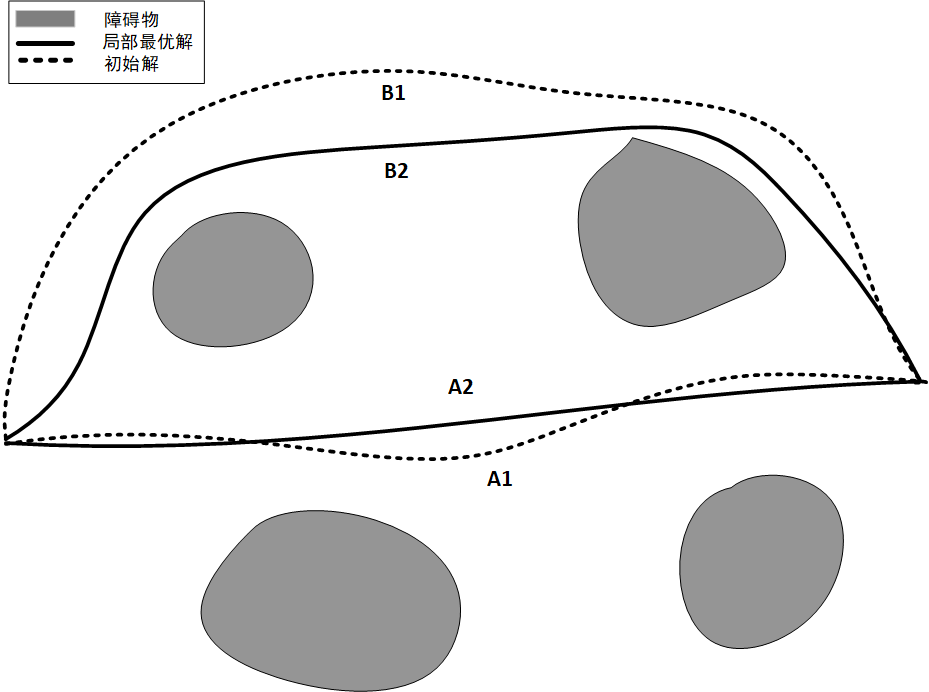
\includegraphics[width=0.8\textwidth]{不同初解.png}
			\caption{不同初始轨迹与最后收敛的轨迹比较}
			\label{fig:不同初解}
		\end{figure}
		可以看出,非线性规划算法处理初始轨迹A1后将迭代优化至轨迹A2,而选取初始方案B1时则会收敛于轨迹B2。通过图示对比可明显观察到,采用初始轨迹A1能使系统收敛至路径长度更优的局部极小值。该现象验证了初始参数设定对优化结果具有决定性作用,因此初始解的获取极为关键。

	\section{本章小结}
	本章系统构建了铰接车运动规划的理论框架与求解体系,并通过全局-局部分层规划架构实现任务分解。

	针对铰接车运动学特性,建立低速非侧滑条件下的四维状态模型,推导了前/后桥坐标变换关系与瞬时转向半径方程,为轨迹优化提供核心运动学约束。基于最优控制理论,将轨迹规划问题转化为多约束非线性规划问题,对比解析解法与数值解法的适用性,采用配点法直接优化状态/控制变量,并通过罚函数法处理非凸约束,解决了传统方法在复杂场景下的维度灾难与收敛性问题。

	\chapter{基于微分平坦的铰接车全局轨迹规划方法}
		在第二章介绍了铰接车的运动学模型,并将轨迹规划统一表述为了最优控制问题。在传统的全局规划问题中,例如A*算法和Dijstra算法可以在栅格地图中搜索出路径代价最小的路径。这些全局规划算法针对全向或者差速机器人会非常有效,然而,它们并不会考虑车身的朝向和曲率等信息。因此,面对具有非完整性的机器人来说并不适合。如图\ref{fig:路径规划算法特例},是期望路径和铰接车实际轨迹的对比图。
		\begin{figure}[H]
			\centering
			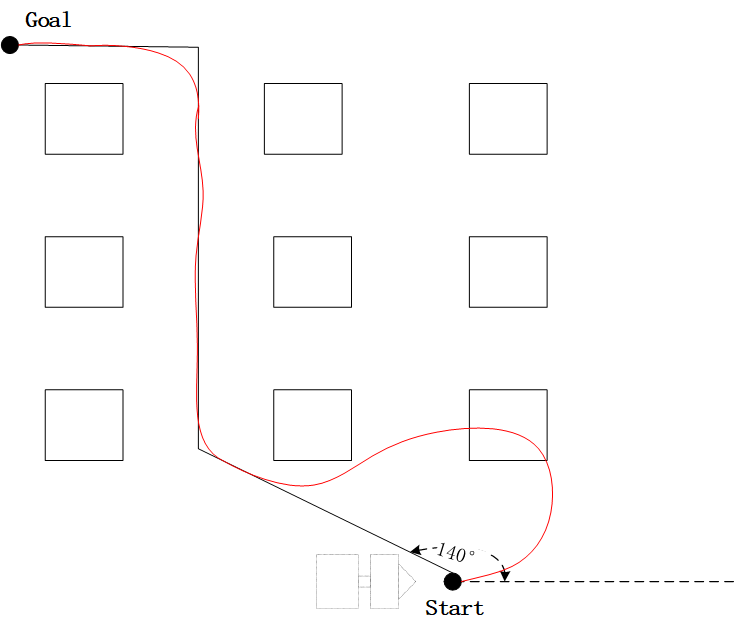
\includegraphics[width=0.8\textwidth]{路径规划算法特例.png}
			\caption{期望路径和实际轨迹对比图}
			\label{fig:路径规划算法特例}
		\end{figure}

		考虑如图\ref{fig:路径规划算法特例}的情况,即需要规划起点Start 到终点Goal 的路径。黑色路径代表了A*算法所规划的理想路径,此路径并没有考虑车辆的初始姿态。实际上,车体的初始朝向与理想路径的起始切线方向之间存在140度的偏差。当车辆尝试沿着这条预设路径行进时,由于初始角度的巨大差异,车辆行驶出了红色的轨迹。最终导致追踪效果极不理想,撞击了障碍物。
		
		本章将基于优化理论和Minco样条,提出一种适用于铰接车辆的全局轨迹优化方法,可以在整段路径上保证严格的转弯半径约束并保证安全躲避碰撞。
		
	\section{铰接模型微分平坦性}
		微分平坦性为非线性控制提供了一种“捷径”,通过平坦输出的参数化,可以将复杂的轨迹优化问题转化为简单的代数计算\upcite{赵昱宇2024基于微分平坦的高超声速飞行器跟踪控制方法}。它在机器人、航空航天和自动化领域有广泛应用,是现代控制理论中连接几何方法与实际工程的重要工具。微分平坦系统具有如下特征\upcite{mellinger2011minimum}:对于一个非线性系统,如果能找一组输出变量,使得所有的状态变量输出变量都可以用这组输出变量及其多阶导数所表示,则这个系统为微分平坦系统。

		对于铰接车而言,实际工作环境往往非常复杂(比如障碍物多、空间狭窄)。这时候做全局轨迹规划可以使用简化的运动学模型,把需要精细调整的部分交给局部规划来处理,以节省计算资源。在这里忽略动态转向,只保留静态转向模型。令$v$和$\gamma$为系统输入,运动学方程(\ref{eq:铰接车运动学模型})可以简化为:
		\begin{equation}
			\begin{aligned}
				\dot{x} &= v\cos\theta\\
				\dot{y} &= v\sin\theta\\
				\dot{\theta} &= v\tan( \gamma /2 ) /L\\
				\dot{\gamma} &= \omega
			\end{aligned}
		\end{equation} 

		对于上述的铰接车的运动模型,选择$x$和$y$作为平坦输出,这在轨迹规划中可以带来很好的性质。$x$和$y$也是需要的轨迹,具有实际的物理意义。
		下面给出铰接车的微分平坦系统:
		\begin{equation}
			\begin{aligned}
				v&=\eta \sqrt{\dot{x}^2+\dot{y}^2}\\
				\theta &=\arctan2( \eta \dot{y},\eta \dot{x} ) \\
				\gamma &=2\arctan( \eta ( \dot{x}\ddot{y}-\dot{y}\ddot{x} ) L/( \dot{x}^2+\dot{y}^2 ) ^{\frac{3}{2}} ) \\
				k&=( \dot{x}\ddot{y}-\dot{y}\ddot{x} ) /( \dot{x}^2+\dot{y}^2 ) ^{\frac{3}{2}}\\
			\end{aligned}
		\end{equation}
	其中,$x$和$y$是系统的平坦输出变量,$\dot{x}$和$\dot{y}$是平坦输出变量关于时间的一阶导数,$\ddot{x}$和$\ddot{y}$是平坦输出变量关于时间的二阶导数。$(v,\theta,\gamma,k)$是选取的状态变量。$k$为轨迹的曲率,也是铰接角的函数。$n\in\{-1,1\}$是车辆运动的方向,分别代表后退和前进两种情况。

	\newpage
	\vspace*{-1.5em}

	\section{轨迹的参数化表达形式}
	在自动驾驶中参数化曲线的方法有很多,例如五次多项式、贝塞尔曲线、B样条、螺旋线、Dubin曲线和RS曲线。Minco曲线作为是一种基于五次多项式的曲线类型,它在处理微分平坦系统上有着天然的优势\upcite{wang2022geometrically}。这一小节将介绍minco曲线的原理,并且运用它处理铰接车的运动规划问题。图\ref{fig:minco}为Minco样条曲线的可视化图。图中$\bm{q}_{0},...,\bm{q}_{N}$为轨迹航点,$\bm{\beta}(t_i)$为第$i$段多项式轨迹。$N$+1个航点一共可以生成$N$段多项式轨迹。
	\begin{figure}[H]
		\centering
		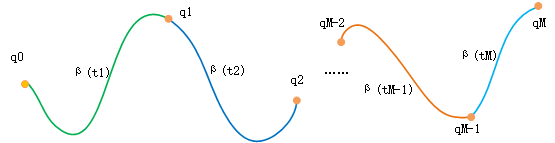
\includegraphics[width=0.9\textwidth]{minco.png}
		\caption{Minco样条曲线}
		\label{fig:minco}
	\end{figure}
		\subsection{Minco样条曲线基本原理}
		在针对minimumJerk(最小化加加速度)形式的优化问题中,其最优解通常表现为一个五次多项式。这种轨迹可以通过多个多项式曲线拼接而成,在自动驾驶技术领域被广泛应用。根据文献\cite{wang2022geometrically}所述,对于微分平坦的系统而言,在平坦输出条件下求得的最优轨迹会表现出更高阶次的连续性。
		
		例如,minimumJerk问题的最优解体现为一个五次多项式。特别地,当系统的运动学模型呈现出微分平坦特性,并使用平坦变量来构建minimumJerk问题,Minco理论进一步证实了平坦变量在snap(即加速度的变化率)这一阶次上具有连续性。由此,基于给定的起点、终点构建边值约束,再确保中间航点满足至snap阶的连续性条件,可以得出轨迹的闭式解。这种特定的闭式解被称为Minco样条曲线。

		接下来,将详细探讨在平坦输出下的两种轨迹优化方法——边值问题(BVP,Boundary Value Problem)和边界与中间值问题(BIVP,Boundary and Intermediate Value)。

		\newpage
		\vspace*{-1.5em}

		(1)BVP

		在多项式规划中一个典型的BVP问题可以表示为:
		\begin{equation}
			\begin{aligned}
				&min\int_0^T{u}(t) ^{\mathrm{T}}\bm{W}u(t) dt\\
				s.t. \ \ \ &z^s(t) =u(t) ,\forall t\in \left[ 0,T \right] \\
				&z^{\left[ s-1 \right]}(0) =\bar{z}_s,z^{\left[ s-1 \right]}(T) =\bar{z}_e
			\end{aligned}
		\end{equation}
		其中,$z(t)$是样条曲线,它可以是上述提到的贝塞尔曲线、B样条或者者多项式形式。$u(t)$是系统的输入,它是$z(t)$关于时间的$s$阶导数。$\bm{W}$是输入代价的权重矩阵。$\bar{z}_s$和$\bar{z}_e$分别是起点状态和终点状态。对于以上最小控制输入问题,控制量$u(t)$是平坦变量的$s$阶次导数,则BVP问题的最优解是一个2$s$-1次多项式\upcite{wang2022geometrically}。

		当$s$等于3时这是一个minimumJerk问题,它的最优解是一个五次多项式。轨迹曲线$z(t)$可以被表示为关于时间$t$多项式函数$\beta(t)$:
		\begin{equation}
			\begin{aligned}
				z&=\beta (t) =\bm{\lambda} ^{\mathrm{T}}(t) \bm{c} =c_0+c_1t+c_2t^2+c_3t^3+c_4t^4+c_5t^5=\\
				&\left[ 1\,\,t\,\,\,\,t^2\,\,t^3\,\,t^4\,\,t^5 \right] \cdot \left[ c_0\,\,c_1\,\,c_2\,\,c_3\,\,c_4\,\,c_5 \right] ^{\mathrm{T}}
			\end{aligned}
		\end{equation}
		其中,$\bm{c}=\left[ c_0\,\,c_1\,\,c_2\,\,c_3\,\,c_4\,\,c_5 \right] ^{\mathrm{T}}$是多项式的系数向量,由各阶系数($c_0,...,c_5$)组成。$\bm{\lambda}(t)=\left[ 1\,\,t\,\,\,\,t^2\,\,t^3\,\,t^4\,\,t^5 \right]^{\mathrm{T}}$。
		
		假设轨迹的时间段是$T$,起点和终点带来的约束可以写为:
		\begin{equation}
			\begin{aligned}
				\left[ \begin{array}{c}
				x_s\\
				v_s\\
				a_s\\
				x_e\\
				v_e\\
				a_e\\
				\end{array} \right] 
				=\underbrace{\begin{bmatrix}
					1&		0&		0&		0&		0&		0\\
					0&		1&		0&		0&		0&		0\\
					0&		0&		2&		0&		0&		0\\
					1&		T&		T^2&		T^3&		T^4&		T^4\\
					0&		1&		2T&		3T^2&		4T^3&		5T^4\\
					0&		0&		2&		6T&		12T^2&		20T^3\\
					\end{bmatrix}}_{\bm{A_F}(t)}  
				\underbrace{\begin{bmatrix}
				c_0\\
				c_1\\
				c_2\\
				c_3\\
				c_4\\
				\end{bmatrix}}_{\bm{c}} 
			\end{aligned}
			\label{eq:BVP}
		\end{equation}
		其中,$x_s,v_s,a_s$分别是轨迹起点的位置、速度和加速度,$x_e,v_e,a_e$对应为终点的状态。需要说明的是,上述讨论的BVP仅针对一维情况。而实际应用中,平坦变量通常是二维的(如平面坐标系中的$x$和$y$方向),此时可以将其分解为两个独立的一维BVP的组合——即分别在$x$和$y$方向求解对应的边界条件,最终通过坐标合成得到二维轨迹。这种解耦方法的核心假设是两个维度在平坦域内无耦合约束。
		
		(2)BIVP 
		
		为了保证轨迹的灵活性,在实际的规划问题中轨迹规划被表述为多个BVP的统一形式,即BIVP问题:
		\begin{equation}
			\begin{aligned}
				\min_{z(t)}\int_{t_0}^{t_N}&u^{\mathrm{T}}(t)\bm{W}u(t)dt\\
				\text{s.t}.z^{( s )}(t) &=u(t) \quad \forall t\in \left[ t_0,t_N \right]\\
				z^{\left[ s-1 \right]}( t_0 ) &=\bar{z}_s,z^{\left[ s-1 \right]}( t_N ) =\bar{z}_e\\
				z^{\left[ d_i-1 \right]}( t_i ) &=\bar{z}_i,1\leq i<N\\
				t_{i-1}&<t_i,1\leq i\leq N.\\
			\end{aligned}
		\end{equation}
		其中,$t_i$为时间变量,$t_0$是起点时刻,$t_N$是终点时刻。$\bm{W}$是输入代价的权重矩阵。$N$为BIVP的区间数目,也就是多项式轨迹的段数。
		其最优性条件指出:对与最小化$s$阶导数的BIVP问题,最优解的单段轨迹一定是一个2$s$-1次多项式,且解具有$s$+1阶导数的连续性。例如,在处理minimumJerk($s$等于3)的轨迹时,轨迹具有snap阶($s$等于4)阶的连续性\upcite{wang2022geometrically}。因此BIVP问题的闭式解可以由起点状态、终点状态、中间位置和中间变量的连续性约束所得到。如图\ref{fig:minco},由$N$+1个航点可以生成$N$段五次多项式轨迹,每个多项式有6个系数,一共有6$N$个系数。这意味着需要6$N$个约束才能唯一确定这个轨迹。
	
		\subsection{起点和终点约束方程} 
		假设共有$N$+1个航点$\bm{q}_{0}$至$\bm{q}_{N}$,其中起点$\bm{q}_{0}=[x_0,y_0,v_{0x},v_{0y},a_{0x},a_{0y}]$和终点$\bm{q}_{N}=[x_N,y_N,v_{Nx},v_{Ny},a_{Nx},a_{Ny}]$完全已知。则起点的约束方程为:
		\begin{equation}
			\begin{aligned}
			\underbrace{\begin{bmatrix}
				x_0&		y_0\\
				v_{0x}&		v_{0y}\\
				a_{0x}&		a_{0y}\\
			\end{bmatrix}}_{\bm{\alpha}_0} 
			 = \underbrace{\begin{bmatrix}
				1&		0&		0&		0&		0&		0\\
				0&		1&		0&		0&		0&		0\\
				0&		0&		2&		0&		0&		0\\
			\end{bmatrix}}_{\bm{F}_0}
			\underbrace{\begin{bmatrix}
				c_{0x}^{1}&		c_{0y}^{1}\\
				c_{1x}^{1}&		c_{1y}^{1}\\
				c_{2x}^{1}&		c_{2y}^{1}\\
				c_{3x}^{1}&		c_{3y}^{1}\\
				c_{4x}^{1}&		c_{4y}^{1}\\
				c_{5x}^{1}&		c_{5y}^{1}\\
			\end{bmatrix}}_{\bm{c}_1}
			\end{aligned}
		\end{equation}
		其中,$c^1_{jx}$为$x$方向上第一段多项式轨迹的第$j$个系数,$c^1_{jy}$为$y$方向上第一段多项式轨迹的第$j$个系数。

		终点的约束方程为:
		\begin{equation}
			\begin{aligned}
			\underbrace{\begin{bmatrix}
				x_N&		y_N\\
				v_{Nx}&		v_{Ny}\\
				a_{Nx}&		a_{Ny}\\
			\end{bmatrix}}_{\bm{\alpha}_N} =
			\underbrace{\begin{bmatrix}
				1&		T_N&		T_N^2&		T_N^3&		T_N^4&    	T_N^5\\
				0&		1&		2T_N&		3T_N^2&		4T_N^3&		5T_N^4\\
				0&		0&		2&		6T_N&		12T_N^2&		20T_N^3\\
			\end{bmatrix}}_{\bm{F}_N} 
			\underbrace{\begin{bmatrix}
				c_{0x}^{N}&		c_{0y}^{N}\\
				c_{1x}^{N}&		c_{1y}^{N}\\
				c_{2x}^{N}&		c_{2y}^{N}\\
				c_{3x}^{N}&		c_{3y}^{N}\\
				c_{4x}^{N}&		c_{4y}^{N}\\
				c_{5x}^{N}&		c_{5y}^{N}\\
			\end{bmatrix}}_{\bm{c}_N} 
			\end{aligned}
		\end{equation}
		其中,$c^N_{jx}$为$x$方向上第$N$段多项式轨迹的第$j$个系数,$c^N_{jy}$为$y$方向上第$N$段多项式轨迹的第$j$个系数。
		
		\subsection{航点的连续性约束方程} 
		除了已知起点和终点之外,还必须保证BIVP问题$N$-1个中间航点的连续性。根据Minco的理论,minimumJerk问题($s$等于3)具有snap阶的连续性。对于每一段多项式轨迹,可以求出它的各阶导数为:
		\begin{equation}
			\begin{aligned}
				\underbrace{\begin{bmatrix}
					x(t)& y(t)\\
					v_x(t)& v_y(t)\\
					a_x(t)& a_y(t)\\
					jerk_x(t)& jerk_y(t)\\
					snap_x(t)& snap_y(t)\\
				\end{bmatrix}}_{\bm{\alpha}(t) }
					= \underbrace{\begin{bmatrix}
						1&		t&		t^2&		t^3&		t^4&		t^5\\
						0&		1&		2t&		3t^2&		4t^3&		5t^4\\
						0&		0&		2&		6t&		12t^2&		20t^3\\
						0&		0&		0&		6&		24t&		60t^2\\
						0&		0&		0&		0&		24&		120t\\
					\end{bmatrix}}_{\bm{G}(t)}
					  \underbrace{\begin{bmatrix}
						c_{0x}^{i}&		c_{0y}^{i}\\
						c_{1x}^{i}&		c_{1y}^{i}\\
						c_{2x}^{i}&		c_{2y}^{i}\\
						c_{3x}^{i}&		c_{3y}^{i}\\
						c_{4x}^{i}&		c_{4y}^{i}\\
						c_{5x}^{i}&		c_{5y}^{i}\\
					\end{bmatrix}}_{\bm{c}_i}
			\end{aligned}
		\end{equation}
		
		则第$i$段轨迹和第$i+1$段轨迹的连续性约束方程可以写为:
		\begin{equation}
			\begin{aligned}
				\bm{G}(T_i)\bm{c}_i-\bm{G}(0)\bm{c}_{i+1} = 0
			\end{aligned}
		\end{equation}
		其中,$T_i$为第$i$段多项式轨迹的时间区间,$\bm{c}_i$为第$i$段多项式轨迹的系数向量。
		由于一共有$N$-1个中间航点,每一个航点带来5个约束,所以连续性约束一共有5$N$-5个。
		
		\subsection{轨迹的闭式解} 
		令中间航点为$\bm{q}_1(x_1,y_1),\bm{q}_2(x_2,y_2),...,\bm{q}_{N-1}(x_{N-1},y_{N-1})$。如果中间航点是已知的,则可以带来$N$-1个航点的位置约束:
		\begin{equation}
			\begin{aligned}
				\bm{q}_i = \begin{bmatrix}
					x(T_i)& y(T_i)
				\end{bmatrix} = \bm{\beta}(T_i)\bm{c}_i
			\end{aligned}
		\end{equation}
		
		现在将中间航点位置约束和连续性约束写在一起:
		\begin{equation}
			\begin{aligned}
				\begin{bmatrix}
					\bm{E}_i &\bm{F}_i
				\end{bmatrix}\begin{bmatrix}
					\bm{c}_i\\
					\bm{c}_{i+1}
				\end{bmatrix}=
				\begin{bmatrix}
					\bm{\beta} ( T_i )& \bm{G}( T_i ) \\
					0 & -\bm{G}( 0 )
				\end{bmatrix}\begin{bmatrix}
					\bm{c}_i\\
					\bm{c}_{i+1}
				\end{bmatrix}  =\begin{bmatrix}
					\bm{q}_i\\
					0
				\end{bmatrix}
			\end{aligned}
		\end{equation}
		综合起点、终点和航点的约束可以得到$6N$个约束方程:
		\begin{equation}
			\begin{aligned}
				\underbrace{\begin{bmatrix}
					\bm{F}_0&		0&		0&		\cdots&		0\\
					\bm{E}_1&		\bm{F}_1&		0&		\cdots&		0\\
					0&		\bm{E}_2&		\bm{F}_2&		\cdots&		0\\
					\vdots&		\vdots&		\vdots&		\ddots&		\vdots\\
					0&		0&		0&		\cdots&		\bm{F}_{N-1}\\
					0&		0&		0&		\cdots&		\bm{E}_N\\
				\end{bmatrix}}_{\bm{M}}
				\underbrace{ \begin{bmatrix}
					\bm{c}_1\\
					\bm{c}_2\\
					\bm{c}_3\\
					\vdots\\
					\bm{c}_{N-1}\\
					\bm{c}_N\\
				\end{bmatrix}}_{\bm{c}} =
				\underbrace{\begin{bmatrix}
					\bm{\alpha}_0\\
					\bm{q}_1\\
					0\\
					\vdots\\
					0\\
					\bm{\alpha_N}\\
				\end{bmatrix}}_{\bm{\alpha}} 
			\end{aligned}
			\label{eq:minco参数化}
		\end{equation}
		其中,$\bm{M}$为维度为$2N\cdot s$的系数方阵,由$\bm{M}$和$\bm{\alpha}$可以唯一确定一组多项式系数$\bm{c}$,即轨迹的参数形式。

		值得一提的是,在$\bm{M}$矩阵中$T_i$是第$i$段多项式的总时间,它可以提前由一些其他的算法来给出,这样$\bm{M}$就是完全已知的矩阵了。由于本章聚焦于路径规划,所以把时间参数$T_i$都归一化处理作为常数。
	
	\section{基于安全走廊的安全约束分析}
	在上一节中已经对铰接车的轨迹进行了参数化,这样就自然的处理了微分方程带来的约束问题,保证了轨迹的平滑性。鉴于施工现场环境复杂多变,地面上可能会出现各种不可预知的障碍物。为了充分利用栅格地图快速索引的优势并增强方案的通用性,本文选用二维空间下的占据栅格地图(Occupancy Grid Map)作为主要的地图类型进行路径规划。
	
	Gao等人\upcite{Gao2018OnlineST}使用固定方向的长方体安全走廊对轨迹进行优化,但是这种方法固定了安全走廊的拓展方向,在障碍物密集的环境中避障效果会大幅削弱。Li等人\upcite{BaiLi:2022}提出的STC(Safe Travel Corridors)算法基于当前路径段的方向进行矩形迭代扩展,生成方式更加灵活。Deits 等人\upcite{Deits:2015}提出了IRIS算法(Iterative Region Inflation by Semidefinite Programming),该方法通过不断膨胀椭球的长短半径,求得与障碍物的切平面,进而构造凸多面体。每次迭代使用最大体积内接椭球作为起始点,然而此过程需要多次求解半正定规划,计算开销较大。Liu 等人\upcite{SikangLiu:2017}提出了SFC算法(Safe Flight Corridors),该算法基于线段不断求解包含该线段且不与障碍物相交的最大椭球,并通过椭球与障碍物的切平面构建凸多面体,从而形成安全走廊。
	
	本文使用不规则凸多边形生成安全走廊,生成方法参考文献\cite{SikangLiu:2017}。它相较于矩形的可以把空间填充的更充实,更逼近于障碍物,从而带来更大的解空间。图\ref{安全走廊比较}是矩形走廊和不规则凸包走廊的对比图。图\ref{fig:凸包矩阵}描述了凸包的线性约束表示方法。
	\begin{figure}[H]
		\centering
		\subcaptionbox{矩形安全走廊\label{安全走廊比较矩形1}}[0.49\textwidth]{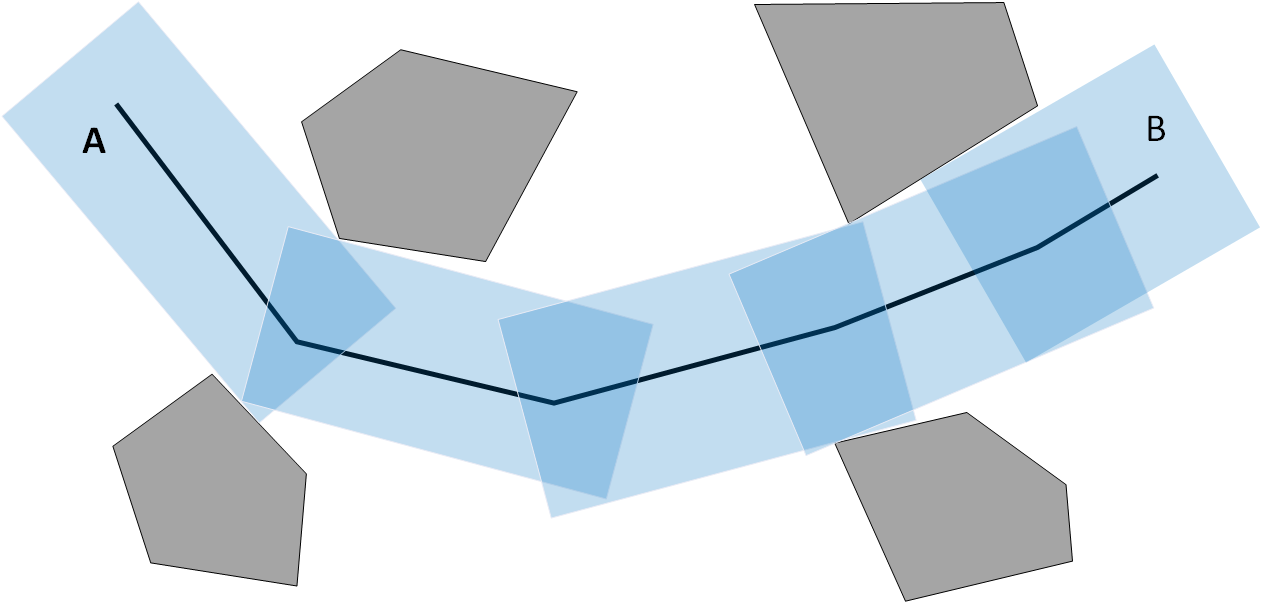
\includegraphics[width=0.4\textwidth]{安全走廊比较矩形1.png}}
		\subcaptionbox{凸多边形安全走廊\label{安全走廊比较多边形2}}[0.49\textwidth]{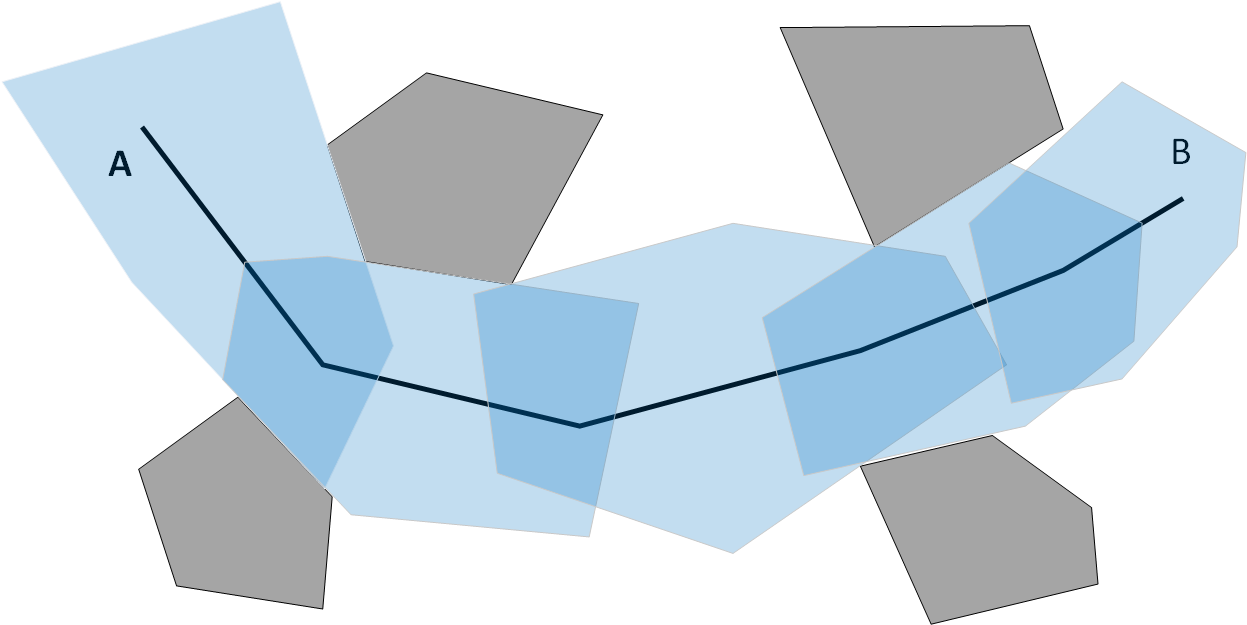
\includegraphics[width=0.4\textwidth]{安全走廊比较多边形2.png}}
		\caption{两种常见的安全走廊比较图}
		\label{安全走廊比较}
	\end{figure}

	\begin{figure}[H]
		\centering
		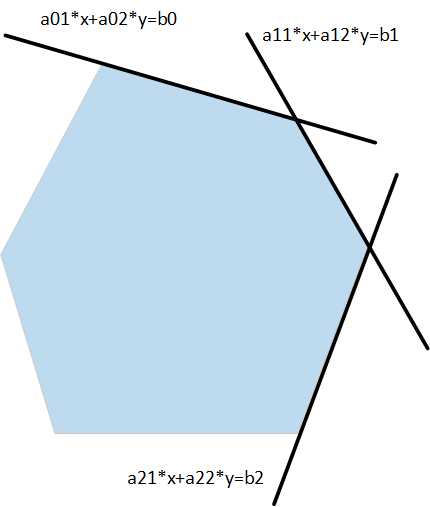
\includegraphics[width=0.3\textwidth]{凸包矩阵.png}
		\caption{凸包与半空间约束关系图}
		\label{fig:凸包矩阵}
	\end{figure}

	凸多边形的区域由一组半空间交集组成。对应2D场景凸包就是由一组直线围成的,如图\ref{fig:凸包矩阵}所示。
	因此,在凸包内的点必然满足以下不等式约束:
	\begin{equation}
		\begin{aligned}
			H_z&=\{\bm{p}\mid \bm{A}\bm{p}<\bm{b}\}\\
			\bm{A}&=\left[ \bm{a}_0,...,\bm{a}_z,...\bm{a}_{n_z-1} \right]^{\mathrm{T}}_{(n_z-1)\times 2},\bm{b}=\left[ b_0,...,b_z,...,b_{n_z-1} \right]^{\mathrm{T}}_{(n_z-1)\times 1}
		\end{aligned}
		\label{eq:走廊约束}
	\end{equation}
	其中,$\bm{p}$为凸包内的点,$\bm{a}_i$是第$i$个半空间的法向量,$\bm{a}_i$和$b_i$唯一去确定一个超平面约束。对于任意在多边形内的点应当满足式(\ref{eq:走廊约束})带来的不等式约束。
	
	\section{点到点全局轨迹规划}
	在3.2节中,介绍了Minco曲线的参数化方法。针对全局轨迹规划并不需要时间维度的信息,重点关注路径层面的两个核心约束条件:首先是路径曲率必须满足由铰接车最大转向角推导出的最小曲率,其次是路径须满足避障要求。关于避障约束的实现细节,已在3.3节通过安全走廊构造方法进行了系统阐述。
		\subsection{铰接车的最大曲率}
		常见的路径规划算法生成的路径常常包含尖锐拐角,这对具有转向半径限制的车辆而言难以准确跟踪。因此,在进行轨迹规划时,必须充分考虑转向半径的约束条件。这样做不仅避免了路径中出现车辆无法执行的急转弯,还提升了路径的整体实用性和车辆运行的安全性,确保所规划的路径符合车辆的实际物理特性。

		对于铰接式车辆来说,其最大曲率主要由静态转向模型决定,这意味着车辆能够达到的最大转向角度是可以精确计算出来的。忽略动态转向带来的曲率影响,铰接式车辆的最大曲率由静态转向模型确定。因此在进行轨迹规划时必须考虑最大曲率的约束条件:
		\begin{equation}
			\begin{aligned}
				k_{max}=\frac{1}{R_{min}}=\frac{\tan( \gamma _{max}/2 )}{L}
			\end{aligned}
			\label{eq:kmax}
		\end{equation}
		其中,$R_{min}$为最小转弯半径,$\gamma_{max}$为最大铰接角。

		在基于样条曲线的路径规划方法中,需通过公式(\ref{eq:kmax})计算的边界条件对曲线曲率施加约束。曲线曲率的计算公式为:
		\begin{equation}
			\begin{aligned}
				k=( \dot{x}\ddot{y}-\dot{y}\ddot{x} ) /( \dot{x}^2+\dot{y}^2 ) ^{\frac{3}{2}}
			\end{aligned}
		\end{equation}
		令坐标向量$\bm{p} =[x,y]^{\mathrm{T}}$,由参考文献\cite{han2023efficient},可以得到曲率的矩阵表达形式:
		\begin{equation}
			\begin{aligned}
				k=\frac{\ddot{\bm{p}}^{\mathrm{T}}\bm{B}\dot{\bm{p}}}{\lVert \bm{p} \rVert _{2}^{3}},\bm{B}=\left[ \begin{matrix}
					0&		-1\\
					1&		0\\
				\end{matrix} \right]
			\end{aligned}
			\label{eq:曲线曲率k}
		\end{equation}
		\begin{equation}
			\begin{aligned}
				\frac{\partial k}{\partial \dot{\bm{p}}}&=\frac{\bm{B}^{\mathrm{T}}\ddot{\bm{p}}}{||\dot{\bm{p}}||_{2}^{3}}-3\frac{\ddot{\bm{p}}^{\mathrm{T}}\bm{B}\dot{\bm{p}}}{||\dot{\bm{p}}||_{2}^{5}}\dot{\bm{p}}\\
				\frac{\partial k}{\partial \ddot{\bm{p}}}&=\frac{\bm{B}\dot{\bm{p}}}{||\dot{\bm{p}}||_{2}^{3}}
			\end{aligned}
		\end{equation}

		\subsection{优化问题的建立}
		根据式(\ref{eq:minco参数化}),轨迹的参数可以由两个要素唯一确定:航点向量$\bm{\alpha}$与系数矩阵$\bm{M}$。由于这两个参数能够唯一表征整条轨迹,在构建优化问题时,将航点向量$\bm{\alpha}$直接做为优化变量是很自然的选择。同时把曲率和安全约束离散化的施加在问题中,当离散化的点足够多时轨迹就是足够安全的。于是可以得到以下优化问题的表达形式:
		\begin{equation}
			\begin{aligned}
				&\min_{\bm{q}_1,...,\bm{q}_{N-1}} J( \bm{q} ) \\
				s.t.&-k_{m}-k_{ij}\le 0\\
				&k_{ij}-k_{m}\le 0 \\
				&\bm{A}_i\bm{p}_{ij}-\bm{b}_{i}<0,\ \ i\in \left[ 1,N \right] ,j\in \left[ 1,m_i \right] 
			\end{aligned}
		\end{equation}
		其中,$k_{m}$是最大曲率,$k_{ij}$的计算方法见公式\ref{eq:曲线曲率k}。$N$是轨迹的段数,$m_i$是第$i$段轨迹的离散点数。$\bm{p}_{ij}=\bm{\beta}^{\mathrm{T}}(\frac{T_i}{m_i}\cdot j)\cdot \bm{c}_i$,是第$i$段多项式轨迹的第$j$个点,$\bm{c}_i$通过$\bm{c} = \bm{M}^{-1}\bm{\alpha}$计算得到。


		针对于曲率和安全这两个不等式约束,引入一个松弛函数将它们作为软约束加入到代价中,松弛函数为:
		\begin{equation}
			\begin{aligned}
				S( x ) =\left\{ \begin{matrix}
					0&		x\le 0\\
					-\frac{1}{2a^3}x^4+\frac{1}{a^2}x^3&		0<x\le a\\
					x-\frac{a}{2}&		a<x\\
				\end{matrix} \right.  \\
					S^{'}(x) = \left\{\begin{matrix}
					0& x\le0 \\
					-\frac{2}{a^3}x^3+\frac{3}{a^2}x^2& 0 < x \le a \\
					1& a < x
				\end{matrix}\right.
			\end{aligned}
			\label{eq:松弛函数}
		\end{equation}
		其中,$a$是一个已知参数,一般选取为优化问题迭代的停止条件值,本文设置的$a$为0.05。$S^{'}(x)$是$S(x)$的导数。如图\ref{fig:松弛函数图},是松弛函数和其导数图。
		\begin{figure}[H]
			\centering
			\subcaptionbox{松弛函数曲线\label{松弛函数}}[0.49\textwidth]{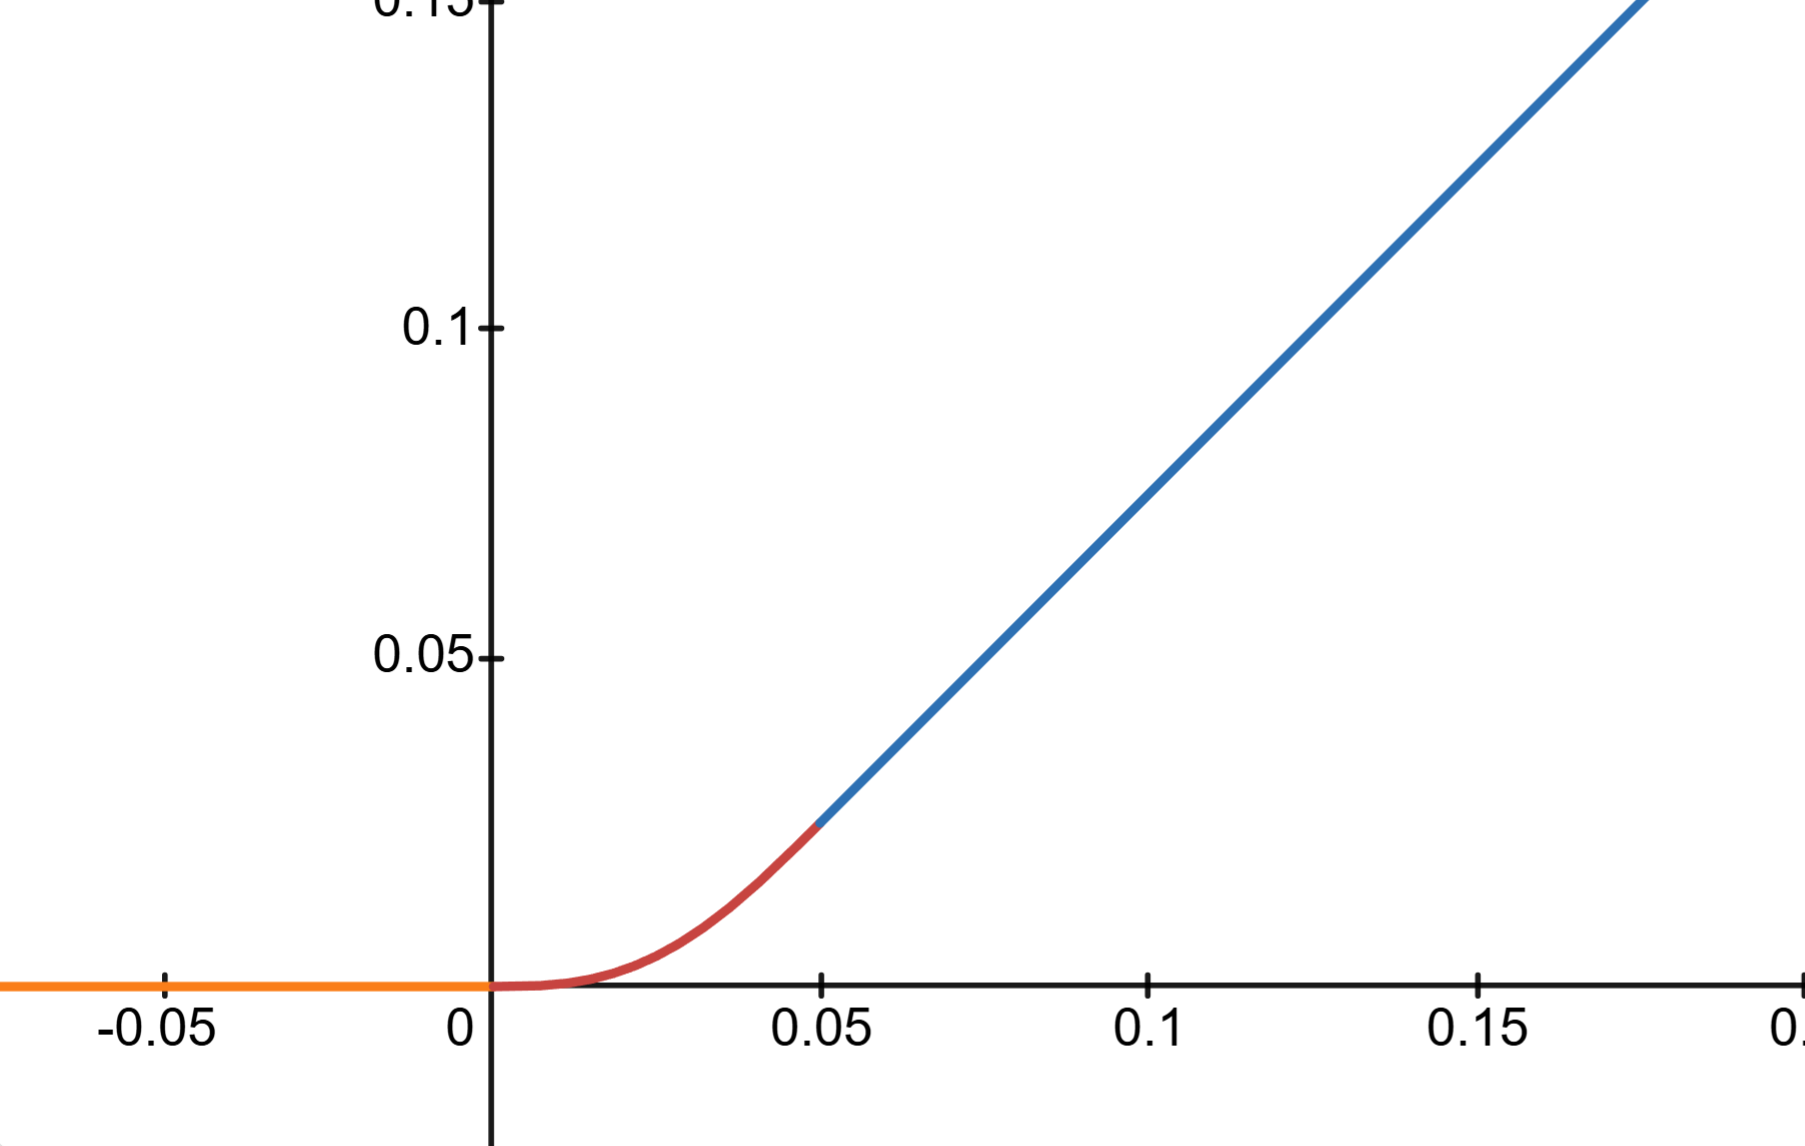
\includegraphics[width=0.4\textwidth]{松弛函数.png}}
			\subcaptionbox{松弛函数导数曲线\label{松弛导数}}[0.49\textwidth]{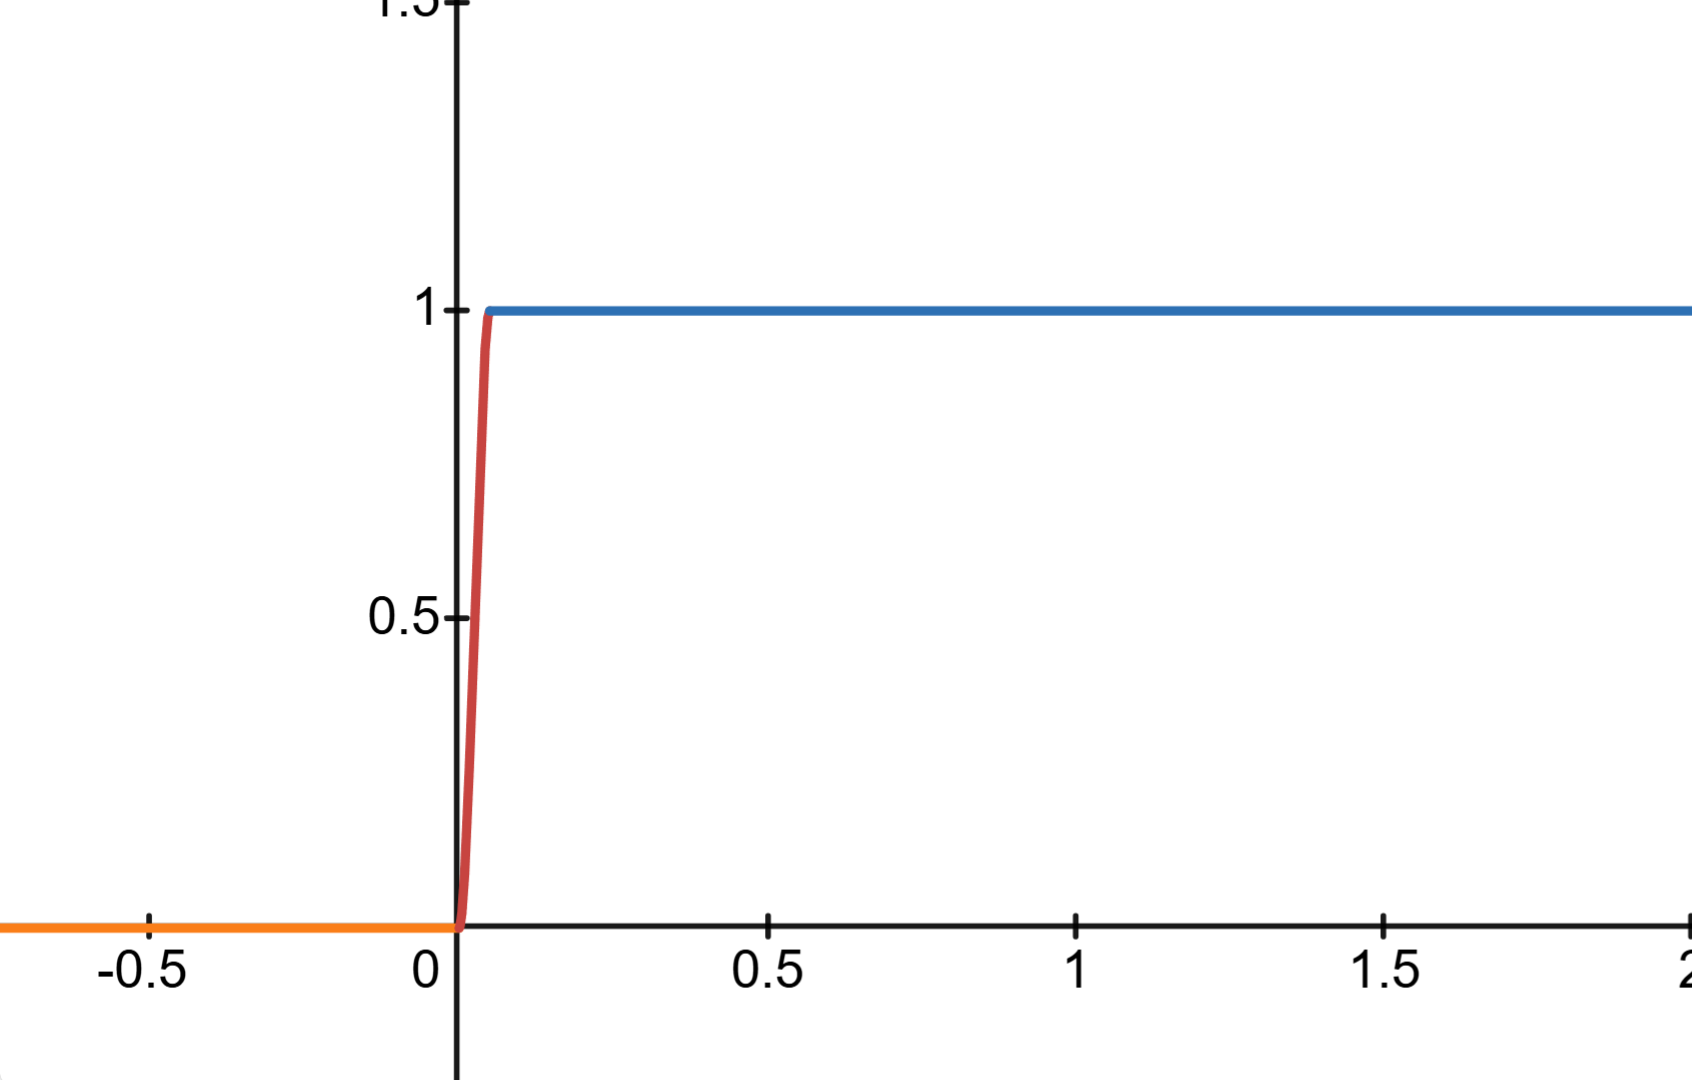
\includegraphics[width=0.4\textwidth]{松弛导数.png}}
			\caption{松弛函数和其导数图}
			\label{fig:松弛函数图}
		\end{figure}

		松弛函数在$x$的负半轴的值为0,也就意味着不等式约束的代价为0。在$0<x \le a$时,代价以一个四次函数上升,越靠近原点代价越小。当$x>a$时代价值以斜率为1直线上升。另外这个分段函数还有非常好的一个特性,在定义域上是$C_2$微分同胚的。这就意味着它的梯度和Hessian矩阵是完全连续的,在优化时不必考虑额外的光滑函数。
		综上,问题被转化成了一个无约束的优化问题:
		\begin{equation}
			\begin{aligned}
				\min_{\bm{q}_1,\bm{q}_2,...,\bm{q}_{N-1}}  J( \bm{q} ) = \sum_{i=1}^N{\sum_{j=1}^{m_i}w_k\cdot{S( -k_m-k_{ij} ) +w_k\cdot S( -k_m+k_{ij} ) +w_c\cdot S( \bm{A}_i\bm{p}_{ij}-\bm{b}_{i})}}
			\end{aligned}
			\label{eq:单阶无约束优化代价}
		\end{equation}
		其中,$w_k$为曲率约束违反的惩罚权重,$w_c$为走廊约束违反的惩罚权重。

		利用矩阵求导的链式法则可以求得各个部分的梯度信息,注意本文矩阵求导法则遵循分母布局。
		\begin{equation}
			\begin{aligned}
				\frac{\partial S( -k_m-k_{ij} )}{\partial \bm{c}_i}&=-( \frac{\partial \dot{\bm{p}}_{ij}}{\partial \bm{c}_i}\frac{\partial k_{ij}}{\partial \bm{\dot{\bm{p}}_{ij}}}+\frac{\partial \ddot{\bm{p}}_{ij}}{\partial \bm{c}_i}\frac{\partial k_{ij}}{\partial \ddot{\bm{p}}_{ij}} ) S^{'} ( -k_m-k_{ij} ) \\
				\frac{\partial S( -k_m+k_{ij} )}{\partial \bm{c}_i}&=( \frac{\partial \bm{\dot{\bm{p}}_{ij}}}{\partial \bm{c}_i}\frac{\partial k_{ij}}{\partial \bm{\dot{\bm{p}}_{ij}}}+\frac{\partial \ddot{\bm{p}}_{ij}}{\partial \bm{c}_i}\frac{\partial k_{ij}}{\partial \ddot{\bm{p}}_{ij}} ) S^{'} ( -k_m+k_{ij} ) \\
				\frac{\partial S( \bm{A}_i\bm{p}_{ij}-\bm{b}_{i} )}{\partial \bm{c}_i}&=\frac{\partial \bm{p}_{ij}}{\partial \bm{c}_i}\bm{A}_{i}^{\mathrm{T}}S^{'}( \bm{A}_i\bm{p}_{ij}-\bm{b}_{i} ) 
			\end{aligned}
		\end{equation}
		其中,$\dot{\bm{p}}$和$\ddot{\bm{p}}$分别为$\bm{p}$对时间的一阶、二阶导数。利用上式求出了$J$关于$\bm{c}$的梯度,于是由$\bm{\alpha} = \bm{M}\bm{c}$,可以推导出:$\frac{\partial \bm{\alpha}}{\partial \bm{q}}\bm{M}^{-T}=\frac{\partial \bm{c}}{\partial \bm{q}}$ ,因此$J$关于$q$的梯度为:
		\begin{equation}
			\frac{\partial J}{\partial \bm{q}}=\frac{\partial \bm{c}}{\partial \bm{q}}\frac{\partial J}{\partial \bm{c}}
		\end{equation}

		\newpage
		\vspace*{-1.5em}

		\subsection{起点和终点航向角保证}
		同样对于给定起点$start(x_s,y_s,v_s,a_s)$和终点$end(x_e,y_e,v_e,a_e)$,需要计算出$x$和$y$两个方向上的初始状态分量。对应为起点$\bm{q}_{0}=[x_0,y_0,v_{0x},v_{0y},a_{0x},a_{0y}]$和终点$\bm{q}_{N}=[x_N,y_N,v_{Nx},v_{Ny},a_{Nx},a_{Ny}]$。 其中,加速度的分解值令其为0,这在路径规划中是合理的。但是对于速度的分解还需要详细讨论,因为其涉及到航向角$\theta$。

		由运动学模型可以求得$x$和$y$方向上的速度分量:
		\begin{equation}
			\begin{aligned}
				v_{0x}=v_s\cos\theta _s\\
				v_{0y}=v_s\sin\theta _s\\
			\end{aligned}
		\end{equation}
		其中,$\theta_s$是铰接车的起始航向角。对于初始速度$v_s$不为零的情况,$v_{0x},v_{0y}$都不等于零,带入优化问题就可以直接保证车辆初始朝向和轨迹的起点切向在一条直线上。但是当$v_{s}=0$时,得到$v_{0x}=0$和$v_{0y}=0$。此时用平坦模型计算$\theta_s$:
		\begin{equation}
			\theta_s=\arctan2 \left( v_{sy},v_{sx} \right) =\arctan2\left( 0,0 \right) 
		\end{equation}
		这时发现其实当$v_{s}=0$时轨迹曲线的切线方向是没有定义的,这是一个奇异点。为了处理这种奇异情况,需要给$v_{s}$加上一个微小正量$\epsilon$保证它的有效性:
		\begin{equation}
			\begin{aligned}
			v_{0x}&=\left( v_s+\epsilon \right) \cos\theta_s\\
			v_{0y}&=\left( v_s+\epsilon \right) \sin\theta_s,0<\epsilon <1e-5
			\end{aligned}
		\end{equation}
		这样就可以保证车辆的起点朝向施加在轨迹上,同样由于$\epsilon$是一个极小量,它几乎不会影响轨迹起点的初始速度。对于终点的处理方法和起点一样。

		\subsection{优化问题求解}
		对于如式\ref{eq:单阶无约束优化代价}的无约束优化问题,有很多成熟的算法可以求解,例如最速下降法、牛顿法、共轭梯度法等。一般的优化算法总体上可以分为两类,一类是基于一阶信息的梯度法,另一类是基于二阶信息的牛顿法。牛顿法除了需要提供代价函数的梯度信息以外,还需要提供代价函数的Hessian矩阵。对于复杂优化问题而言解析计算Hessian是非常困难的。
		
		L-BFGS算法作为一种高效的拟牛顿优化方法,在优化过程中会不断地迭代逼近出一个Hessian矩阵,省去了手动推导的难度\upcite{liu1989limited}。在大规模无约束优化问题中有显著的优势。其核心优势在于内存效率和计算效率,仅存储最近的迭代信息,有效处理高维问题,同时快速收敛于最优解。综合众多因素本文选择使用L-BFGS优化算法最为本优化问题的优化求解算法。

		由于使用优化的方法生成轨迹,所以需要一个快速生成航点的路径规划算法,为算法提供软起动初值。对于这个路径规划算法一般并不会去关心是否最优,但是它需要以较低的时间复杂度运行,因为优化过程可以带来足够的最优性。在本文中使用RRT-Connect生成路径。区别于传统的RRT算法,RRT-Connect同时从起点和终点搜索路径,可以显著提高搜索的效率,减少搜索的次数。局部规划算法的步骤如下:

		第一,初始解的构造。使用RRT-Connect算法搜索出从起点到终点的一条路径$\bm{\hat{path}}$,其中包含$N$+1个路径点。
		\begin{equation}
			\begin{aligned}
				\bm{\hat{path}} = \begin{bmatrix}
					x_0 &y_0\\
					x_1&y_1\\
					...\\
					x_N& y_N
				\end{bmatrix} 
			\end{aligned}
		\end{equation}
		由此可以构造初始解$\bm{\bar{q}}_{init}
		=\begin{bmatrix}
			\bm{q}_1& \bm{q}_2& ...&\bm{q}_{N-1}
		\end{bmatrix}^{\mathrm{T}}$。

		第二,构造系数矩阵$\bm{M}$。将时间变量$T_i$归一化,则$\bm{M}$矩阵是完全一已知的。对于系$\bm{\alpha}$中的$\bm{\alpha}_0$和$\bm{\alpha}_N$可以通过起点$\bm{q}_0$和终点$\bm{q}_N$构建。
		
		第三,构造安全走廊。沿着路径$\bm{\hat{path}}$膨胀出安全走廊。

		第四,构建代价函数、构建梯度函数,送入求解器求解得到最优解$\bm{q}_{opt}$。

		第五,获取最优路径参数$\bm{c}$。通过$\bm{q}_{opt}$构建$\bm{\alpha}$,再通过$\bm{c} = \bm{M}^{-1}\bm{\alpha}$得到系数$\bm{c}$。

		第六,得到路径最优表达式。$\bm{path}(t_i)=\bm{\beta}(t_i)\bm{c}_i$,其中$t_i$是第$i$条轨迹多项式中的时刻,$0 \le t_i \le 1$。通过这个公式采样可以得到离散的轨迹。
		
		% 下面给出全局规划算法的伪代码:
		%  \begin{algorithm}  
		%  	\caption{Global Planning}  
		%  	\label{alg:global_planning}  
		%  	\begin{algorithmic}[1]  
		%  		\REQUIRE  
		%  		$\bm{p}_{start},\bm{p}_{end},\bm{map}$
		%  		\ENSURE  
		%  		$\bm{path}$
		%  		\STATE $\hat{\bm{path}},\bm{q}_{init} \leftarrow RRT-Connect(\bm{p}_{start},\bm{p}_{end},\bm{map})$
		%  		\STATE $corridor \leftarrow getCorridor(\bm{map},\hat{\bm{path}})$
		%  		\STATE $cons \leftarrow getConstraint(\bm{M},\kappa_{min,max},cors)$
		%  		\STATE $cosFcn \leftarrow getCost(cons)$
		%  		\STATE $grad \leftarrow getGrad(cons)$ \\
		%  		\STATE $\bm{q}_{opt} \leftarrow \mathbf{lbfgs}(\bm{q}_{init},cosFcn,grad)$
		% 		\STATE $\bm{c} = \bm{M}^{-1}\bm{\alpha}$, $\bm{\alpha} \longleftarrow \bm{q}_{opt}$
		% 		\RETURN $\bm{path}(t_i)=\bm{\beta}(t_i)\bm{c}_i$
		%  	\end{algorithmic}  
		%  \end{algorithm}
		
	\section{多站点航行全局轨迹规划}
	在上一节中描述了完整的算法结构和细节,可以完成一个点对点的路径规划问题。对于一些更加复杂的场景,例如码头搬运、舱体清卸、矿山运料等多种复杂的工况下,铰接车需要依次去往各个区域规定完成卸货。这样的场景往往需要面向任务设计一个框架。因为这些场景需要更灵活的运动模式,例如倒车。这一节将针对码头搬运场景设计一个周期性的规划流程,也称多站点航行全局轨迹规划。图\ref{fig:全局规划}展示的是一个多站点搬运示意图。
	\begin{figure}[H]
		\centering
		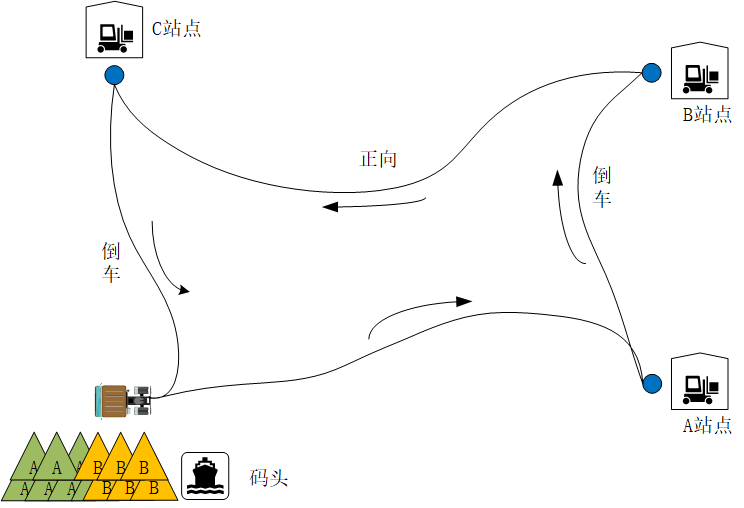
\includegraphics[width=0.8\textwidth]{全局规划.png}
		\caption{多站点场景下全局规划示意图}
		\label{fig:全局规划}
	\end{figure}
		\subsection{多站点航行规划的问题描述}
		考虑图\ref{fig:全局规划}的搬运问题,需要铰接车从码头出发,装货完成去往A点进行卸货,然后去往B点,再去C点,最后回到码头重新装货。这个搬运周期一共需要四次规划,且搬运过程中由于环境等因素规划过程需要倒车。在整个规划周期中铰接车一共需要经过四个站点,分别为码头、A站点、B站点和C站点。在整个过程中受到路径受到两个方面的限制。第一,每一段轨迹的起点的切线方向必须和铰接车保持一致,这就是车辆的非完整约束,这在上一节中已经处理。第二,如果在站点处需要求车辆发生换向,则换向后的轨迹的航向和换向前应该相反。 
		

		\subsection{站点的换向处理}
		如图\ref{fig:换向1}和图\ref{fig:换向2},在中间站点处的是否换向包含两种情况。一种是站点前的车辆运动方向和站点后运动方向相同,则不需要换向。另一种是站点前的车辆运动方向和站点后运动方向相反,则需要换向,此站点也被称为换向点。

		\newpage
		\vspace*{-1.0em}

		\begin{figure}[H]
			\centering
			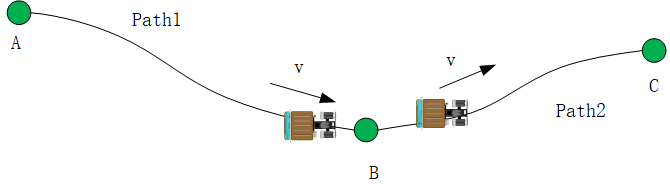
\includegraphics[width=0.8\textwidth]{换向1.png}
			\caption{B点不需要换向}
			\label{fig:换向1}
		\end{figure}
		\begin{figure}[H]
			\centering
			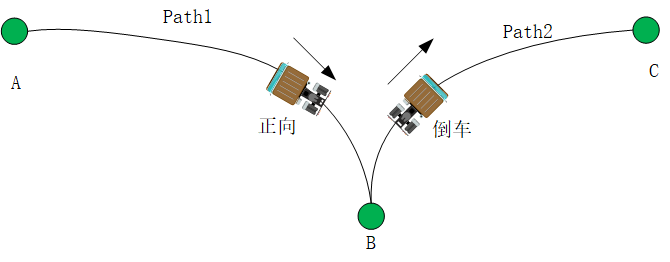
\includegraphics[width=0.8\textwidth]{换向2.png}
			\caption{B点完成换向}
			\label{fig:换向2}
		\end{figure}

		图\ref{fig:换向1}是表示的是车正向行驶穿越站点的情况,经过站点时不用倒车。在规划AB段路径时B点作为终点,在规划BC段路径时B点作为起点车辆的运动方向和车辆的朝向相同。图\ref{fig:换向2}是表示的是车正向行驶到达站点,再反向倒车。与图\ref{fig:换向1}不同的是,在规划BC段路径时B点作为起点车辆的运动方向和车辆的朝向相反,而AB段相同,因此规划BC段时B点作为起点需要换向。

	\section{本章小结}
	本章针对铰接车辆的轨迹规划难题,提出了一种基于微分平坦理论与Minco样条的全局优化方法,通过多维度约束融合与高效求解策略,实现了符合运动学特性、安全避障与实时性的规划框架。首先基于铰接车简化运动学模型,选取笛卡尔坐标作为微分平坦输出,推导出包含速度、航向角、铰接角及曲率的显式表达式,将非完整约束转化为平坦空间代数关系。其次,采用Minco样条对轨迹进行参数化建模,通过建立包含起点/终点状态、中间航点位置及高阶导数连续性的BIVP约束体系,得出基于航点向量的闭式解形式。针对避障需求,设计基于安全走廊的生成机制,通过凸多边形约束实现障碍物规避。进一步提出曲率约束松弛函数,将铰接角物理极限映射为轨迹曲率硬约束,构建包含安全走廊与运动学约束的非线性优化模型,利用L-BFGS算法实现高效求解。在下一章中将针对精细化的避障,介绍局部规划方法。
	
	\chapter{基于安全走廊的铰接车局部轨迹规划方法}
	在第三章中介绍了铰接车的全局轨迹规划方法。本章将提出基于安全走廊的时空联合局部轨迹规划方法。全局与局部规划共同构成完整的运动规划系统。

	首先,对铰接车几何结构进行建模,以提升碰撞检测速度。其次,针对铰接车特点提出改进的Hybrid A*算法,用于局部轨迹规划的热启动。接着,对规划问题涉及的所有约束进行处理。最后,针对最终优化问题进行求解。

	\section{铰接车的几何结构建模}
	为了保持优化问题的凸性,将车辆底盘形状建模为两个矩形的连接,从而将铰接车的避障问题转化为多边形几何碰撞问题。如图\ref{fig:铰接车外观结构建模}所示,车辆形状分为前轴和后轴两部分,共由九个顶点A、B、C、...、H和O1。
	\begin{figure}[H]
		\centering
		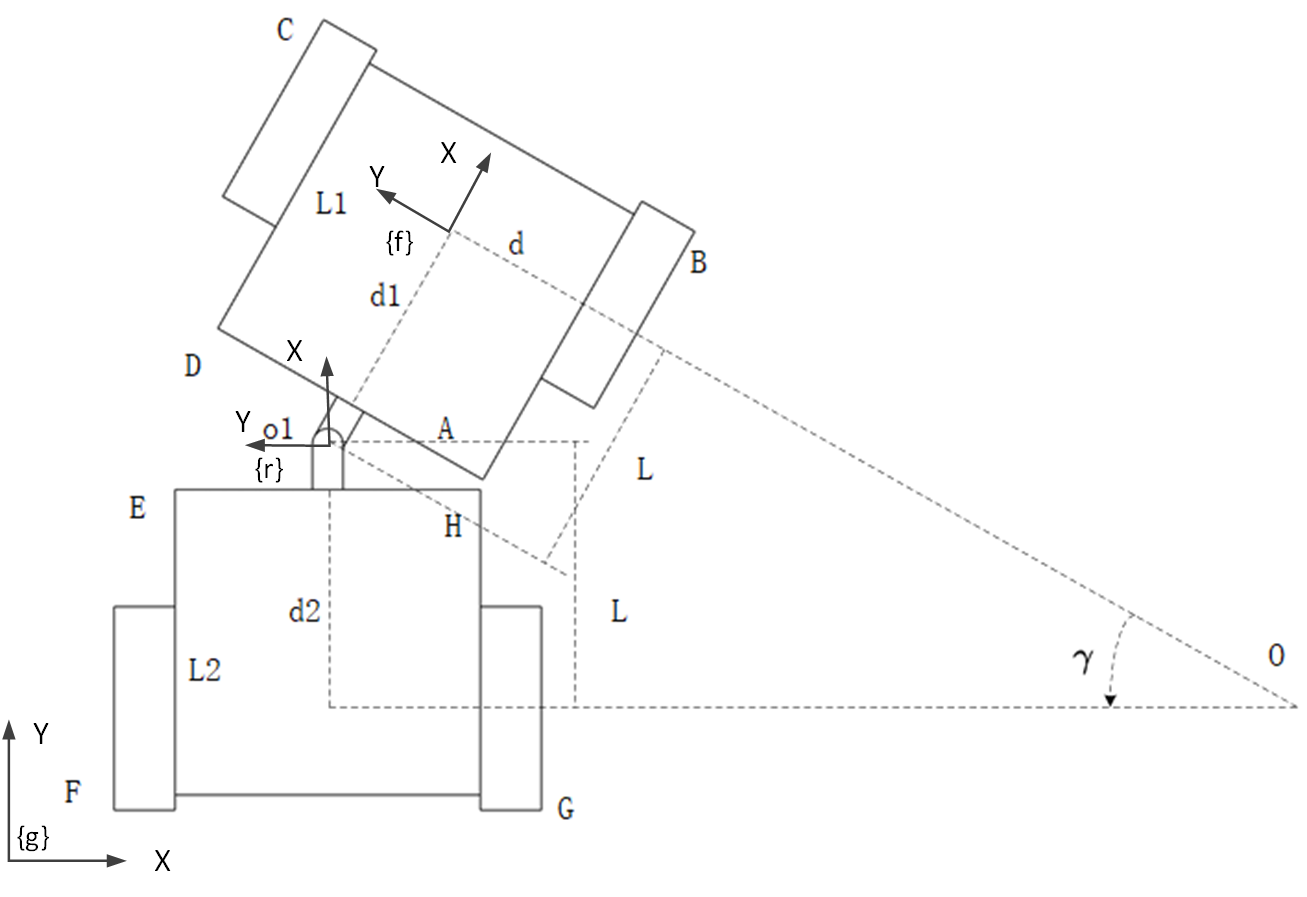
\includegraphics[width=0.8\textwidth]{铰接车几何结构.png}
		\caption{铰接式车辆结构建模}
		\label{fig:铰接车外观结构建模}
	\end{figure}
	图中$\{f\}$、$\{r\}$和$\{g\}$分别为前桥坐标系、后桥坐标系和世界坐标系。与动学模型相一致,选取前桥中点作为参考点$(x,y)$,沿着车体方向作为x轴正方向。则A、B、C、D、O1相对于前桥坐标系$\{f\}$和E、F、G、H的相对后桥坐标系$\{r\}$的坐标可以表示为:
	\begin{equation}
		\begin{aligned}
			\bm{l}_{A}^{\mathrm{T}}&=( -d_1,-width/2 ) ,\bm{l}_{B}^{\mathrm{T}}=( L_1-L,-width/2 ) \\
			\bm{l}_{C}^{\mathrm{T}}&=( L_1-L,width/2 ) ,\bm{l}_{D}^{\mathrm{T}}=( -d_1,width/2 ) \\
			\bm{l}_{E}^{\mathrm{T}}&=( d_2-L,width/2 ) ,\bm{l}_{F}^{\mathrm{T}}=( -L_2,width/2 ) \\
			\bm{l}_{G}^{\mathrm{T}}&=( -L_2,-width/2 ) ,\bm{l}_{H}^{\mathrm{T}}=( d_2-L,-width/2 ) \\
			\bm{l}_{O_1}^{\mathrm{T}}&=( -L,0 ) 
		\end{aligned}
		\label{eq:铰接车顶点}
	\end{equation}
	其中,$width$为BC的长度。令$\bm{R}_\theta$和$\bm{\sigma}$为世界坐标系到车辆坐标系的旋转矩阵和平移向量,根据式\ref{eq:铰接车顶点},则前桥顶点在世界坐标系下表示为:
	\begin{equation}
	\begin{aligned}
		\varepsilon_f = \left\{ \bm{p}_f \in \mathbb{R}^2 \mid \bm{p}_f=\bm{R}_\theta \bm{l}_f+\bm{\sigma},  f = A,B,C,D \right\},
	\end{aligned} 
	\end{equation}
	其中,$\bm{\sigma}$也是前轴参考点坐标,表示为$\bm{\sigma}=(x,y)$。
	
	$\bm{l}_E,\bm{l}_F,\bm{l}_G,\bm{l}_H$是相对于后桥坐标系下的坐标。在从世界坐标系到后桥坐标系的变换中,还涉及到前桥坐标系,需要应用旋转矩阵$\bm{R}_\theta$和$\bm{R}_\gamma$。平移向量由世界坐标系中的铰接点给出,记为$\bm{\sigma}_1$。可以得到后桥的坐标变换为: 
	\begin{equation}
		\begin{aligned}
				\bm{p}_r&=\bm{R}_\gamma \bm{R}_\theta \bm{l}_b+\bm{\sigma}_1\\
				\bm{\sigma}_1&=\bm{R}_\theta \bm{l}_{O_1}+\bm{\sigma}
		\end{aligned}
	\end{equation}
	则后桥的顶点集表示如下:
	\begin{equation}
		\begin{aligned}
			\varepsilon_r = \left\{ \bm{p}_r \in \mathbb{R}^2 \mid \bm{p}_r=\bm{R}_\gamma \bm{R}_\theta \bm{l}_r+\bm{R}_\theta \bm{l}_{O_1}+\bm{\sigma},r = E,F,G,H.  \right\} \\
		\end{aligned}
	\end{equation}
	其中,$\bm{R}_\theta = \begin{bmatrix}
		\cos\theta &-\sin\theta\\
		\sin\theta &\cos\theta
	\end{bmatrix}$,$\bm{R}_\gamma$同理。

	
	\section{铰接车Hybrid A*算法的改进}
	Hybrid A*算法首次应用于2007年DAPPA城市挑战赛,并由Dolgov等人提出。与传统的A*算法不同,Hybrid A*算法在三维空间中进行搜索,且在搜索过程中,邻居节点的拓展是通过动力学方程的前向推演来实现的。然而,传统的Hybrid A*算法是基于$x-y-\theta$三维空间进行搜索的,这使得它并不适用于铰接车模型。铰接车由于其具有较为复杂的非线性运动特性,因此直接应用传统的Hybrid A*算法会面临难以满足约束条件和路径质量不高的问题。

	为了能够适应铰接车的路径规划问题,本节将提出一种改进Hybrid A*算法。修改Hybrid A*算法中的邻居节点拓展策略,结合铰接车的运动学特性,改进算法的搜索策略,以便更好地在铰接车的状态空间中找到一个次优的初解。该初解将在后续的优化过程中作为起点,进一步引导算法沿着合适的方向优化,最终得到一个更加符合实际需求的路径。通过这种方式,能够克服传统Hybrid A*算法的局限性,为铰接车路径规划提供更为高效和精准的解决方案。
		\subsection{节点拓展策略改进}
		假设铰接车当前的状态为$x_0(x,y,\theta,\gamma)$,一般Hybrid A*算法将控制区间$v_{min}$至$v_{max}$和$\omega_{min}$至$\omega_{max}$进行离散化。并从当前状态$x_0$开始以输入$v$和$\omega$在$\Delta t$时间内进行运动学推演得到下一个状态,运动学推演见式(\ref{eq:铰接车运动学模型})。图\ref{fig:Hybrid A*原始采样策略和改进采样策略}是原始Hybrid A*算法运动学采样策略和改进后的采样策略比较。 
		\begin{figure}[H]
			\centering
			\subcaptionbox{Hybrid A*原始采样策略\label{fig:hybrid采样}}[0.49\textwidth]{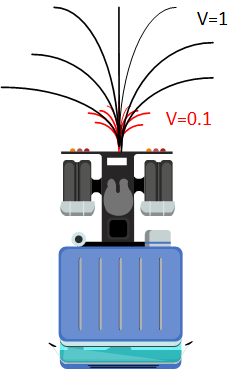
\includegraphics[width=0.2\textwidth]{hybrid采样.png}}
			\subcaptionbox{Hybrid A*改进采样策略\label{fig:hybrid采样改进剪枝}}[0.49\textwidth]{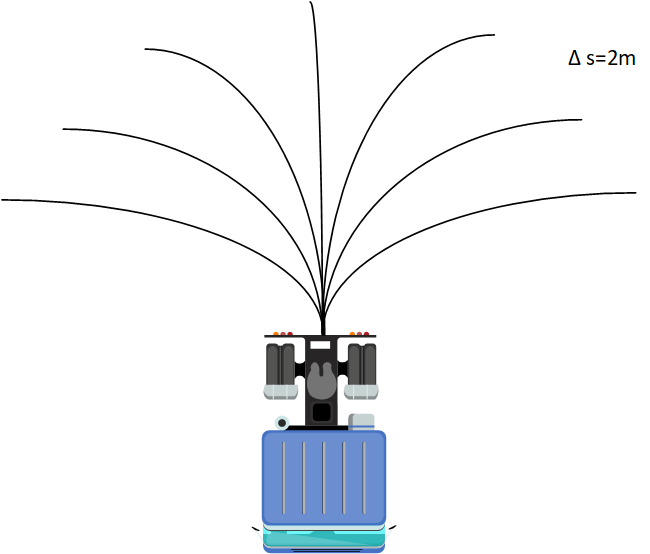
\includegraphics[width=0.5\textwidth]{hybrid采样改进剪枝.png}}
			\caption{Hybrid A*原始采样策略和改进采样策略}
			\label{fig:Hybrid A*原始采样策略和改进采样策略}
		\end{figure}
		如图\ref{fig:Hybrid A*原始采样策略和改进采样策略}\subref{fig:hybrid采样},列出了速度为0.1和1采样点。可以看出这种采样方式在$|v|$很小时,不管$\omega$为多少,所积分出来的轨迹都会聚在一起。红色轨迹有短又聚合,并没有充分的去探索周围空间。这是很浪费计算资源且没有必要的。由于系统的输入是二维($v$和$\omega$),所以算法的时间复杂度是$O(N^2)$。下面将针对节点采样进行改进,可以有效解决采样出来的轨迹聚合的问题,并以$O(N)$时间复杂度完成探索,某种意义上这也是一种轨迹的剪枝策略。 

		首先为了降低计算的复杂度,使用铰接车的静态转向模型,系统的输入为$v$和$\gamma_u$。不再以固定的时间$\Delta t$进行采样,以固定的行驶路程$\Delta s$采样,于是系统的输入为$\gamma_u$。这样做的本质是只在路径几何层面考虑规划问题。运动学方程如下:
		\begin{equation}
			\begin{aligned}
				\left[ \begin{array}{c}
					x_{k+1}\\
					y_{k+1}\\
					\theta _{k+1}\\
					\gamma _{k+1}\\
				\end{array} \right] =\left[ \begin{array}{c}
					x_k+\Delta s\cdot \cos\theta _k\\
					y_k+\Delta s\cdot \sin\theta _k\\
					\theta _k+\frac{\Delta s}{L}\cdot \tan (\gamma _{uk}/2 )\\
					\gamma _{uk}\\
				\end{array} \right] 
			\end{aligned}
			\label{eq:改进运动学推演策略}
		\end{equation}
		其中,$\Delta s$是采样的路径步长,$x$、$y$、$\theta$和$\gamma$是铰接车的位形空间状态变量。

		图\ref{fig:Hybrid A*原始采样策略和改进采样策略}\subref{fig:hybrid采样改进剪枝}为$\Delta s$等于2 m的采样过程。可以看出相对于原始推演策略来说这种方式可以大大降低时间复杂度。本质上这其实也是速度$v$为固定常数时的特殊情况。此外为了加速搜索,Hybrid A*在搜索过程中还引入了RS(Reeds-Shepp曲线),进一步提高搜索效率。
		
		RS曲线是一种用于求解二维平面中任意始末位姿之间最短路径的算法。该算法的核心思想是通过分析并归纳所有可能的路径类型,将最短路径的构造问题简化为48种不同的情况,并且对每种情况进行了枚举,涵盖了圆弧和直线段的各种排列组合方式。因此,RS曲线可以为无障碍情况下的最短路径提供解析表达式,并能够快速地构造出符合运动学约束的可行路径。RS曲线特别适用于涉及到转向半径约束的路径规划问题,尤其是在移动机器人和自动驾驶领域中,其广泛应用于生成车辆的路径规划。该算法通过考虑车辆的运动学约束(如最小转弯半径),能够有效地找到从起点到终点的最短路径,并确保路径是可行的,符合实际的转向和行驶要求。值得指出的是,RS曲线在hybrid A*搜索的最后一步具有加速收敛到终点的效果。

		\subsection{代价函数设计}
		Hybrid A*算法在进行节点的扩展时,会从采样出来的节点中选出代价最低的一个节点作为下一个扩展节点。Hybrid A*算法的代价函数$f$分为累积代价$g$和启发式函数代价$h$两个部分,见式(\ref{eq:搜索代价})。
		\begin{equation}
			\begin{aligned}
				f = g+h
			\end{aligned}
			\label{eq:搜索代价}
		\end{equation}
		其中,累积代价$g$表征着起点到当前节点的路程代价,启发式代价$h$表征当前节点到终点的代价。一般当前点到终点的最小代价是未知的,所以理论上启发式函数$h$设计的越靠近最优代价则搜索效果越好。
		
		采样策略的输入变量是$\gamma_u$,由于上一时刻的采样和这一时刻独立,所以可能出现$\Delta {\gamma}$过大的情况,也就是铰接角突变问题,这对于下层控制是不利的。所以在代价函数中必须含有$\Delta {\gamma}$项使得铰接角变化率尽量小,称之为转向惩罚。因此将下一个拓展的累积代价设计为:
		\begin{equation}
			\begin{aligned}
				g_{next}=g_{cur}+ (x_{next}-x_{cur} ) ^2+ (y_{next}-y_{cur} ) ^2+ (\gamma _{u(next)}-\gamma _{u (cur)} ) ^2
			\end{aligned}
		\end{equation}
		其中,$g_{cur}$为当前节点的累积代价,$g_{next}$为即将拓展的邻居节点累积代价。$x_{cur},y_{cur}$为当前节点位置信息,$x_{next},y_{next}$为即将拓展的邻居节点的位置信息。$\gamma _{u(next)}$为从当前节点拓展到邻居节点的所需要的转向输入,$\gamma _{u(cur)}$为从上一节点拓展到当前节点的所需要的转向输入。

		启发式代价函数$h$记录当前节点到终点的估计代价,hybrid A*算法的启发式代价一般分为两个部分:非完整约束启发式代价$h_{nonh}$和避障启发式代价$h_{collision}$。其中非完整约束代价$h_{nonh}$是仅仅在考虑车辆有转弯半径且不考虑障碍物的情况下的距离代价,通常可以直接由RS曲线闭式算出。避障启发式代价$h_{collision}$则是仅考虑避障时的代价,使用无穷范数作为避障启发式代价,见式(\ref{eq:启发代价})。
		\begin{equation}
			\begin{aligned}
				h_{nonh} &= RS(x_{cur},y_{cur},x_{goal},y_{goal})\\
				h_{collision} &= \max( |x_{cur}-x_{goal}|,|y_{cur}-y_{goal}|)\\
				h &= h_{nonh}+h_{collision}
			\end{aligned}
			\label{eq:启发代价}
		\end{equation}

		\subsection{碰撞检测算法设计}
		在碰撞检测算法的设计中,通过检查车辆几何模型与栅格地图的是否有重叠来判断路径可行性,其核心原理基于车辆位姿变换与离散化障碍物检测。首先,算法利用旋转矩阵将车辆初始轮廓坐标变换到全局坐标系下,计算各顶点坐标后转换为地图栅格索引,以便在栅格地图中查询索引处是否由障碍物。随后,对车辆轮廓边进行线段离散化检测。
		
		如图\ref{fig:障碍物检测图}所示,采用Bresenham算法\upcite{bresenham1977linear}遍历每条边的栅格路径,若任一栅格为障碍物或超出地图边界,则判定为碰撞。在路径搜索过程中,该模块嵌入节点扩展和Reeds-Shepp曲线连接阶段,逐段验证候选路径的安全性。其优势在于计算效率高且与栅格地图兼容性强,但受限于离散化误差可能忽略细小障碍物,且仅适用于静态环境。图\ref{fig:障碍物检测图}\subref{fig:bresham_free}为铰接车没有和障碍物发生碰撞的场景,图\ref{fig:障碍物检测图}\subref{fig:bresham_colli}则是发生碰撞的场景,其中红色栅格是车体轮廓和障碍物栅格重叠的区域。
		\begin{figure}[H]
			\centering
			\subcaptionbox{铰接车处于安全区域\label{fig:bresham_free}}[0.49\textwidth]{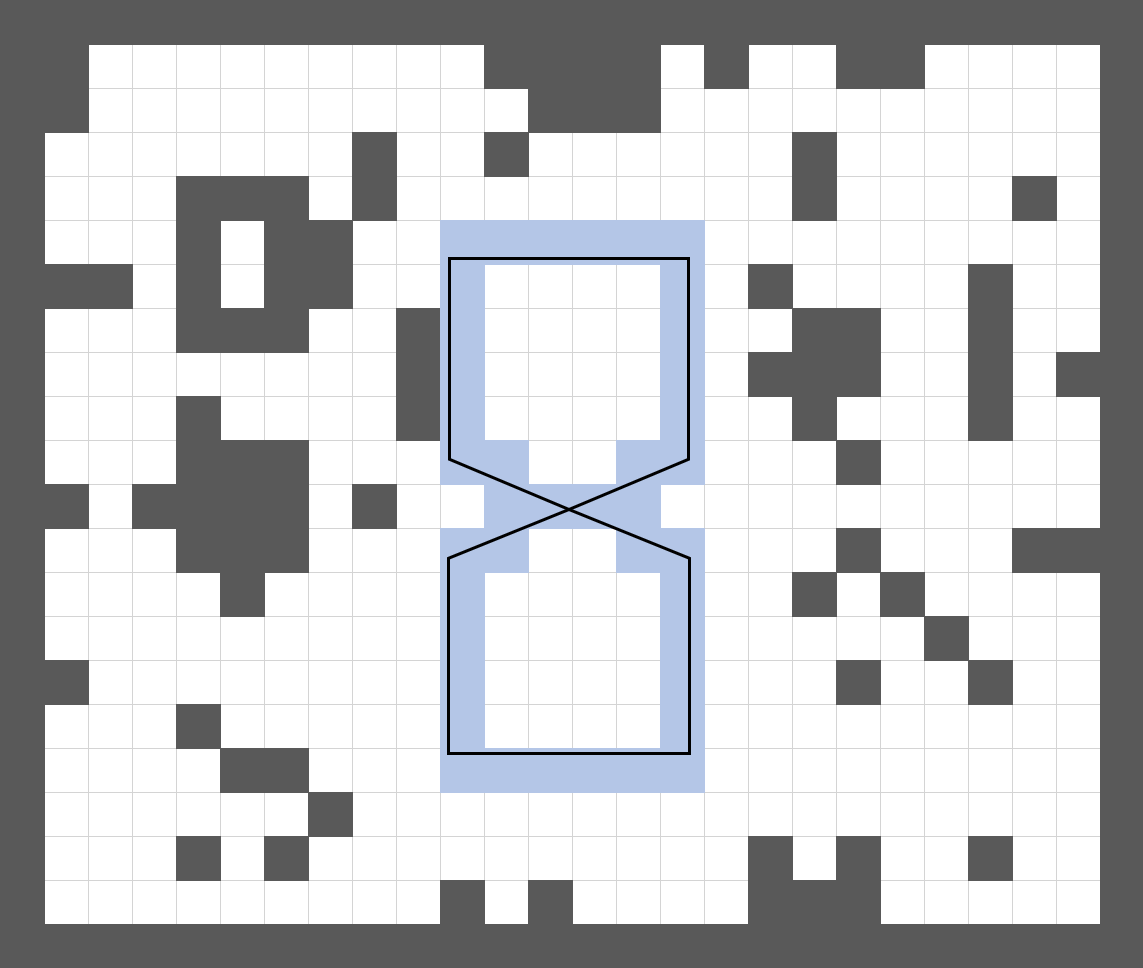
\includegraphics[width=0.4\textwidth]{bresham_free.png}}
			\subcaptionbox{铰接车与障碍物发生重叠 colli\label{fig:bresham_colli}}[0.49\textwidth]{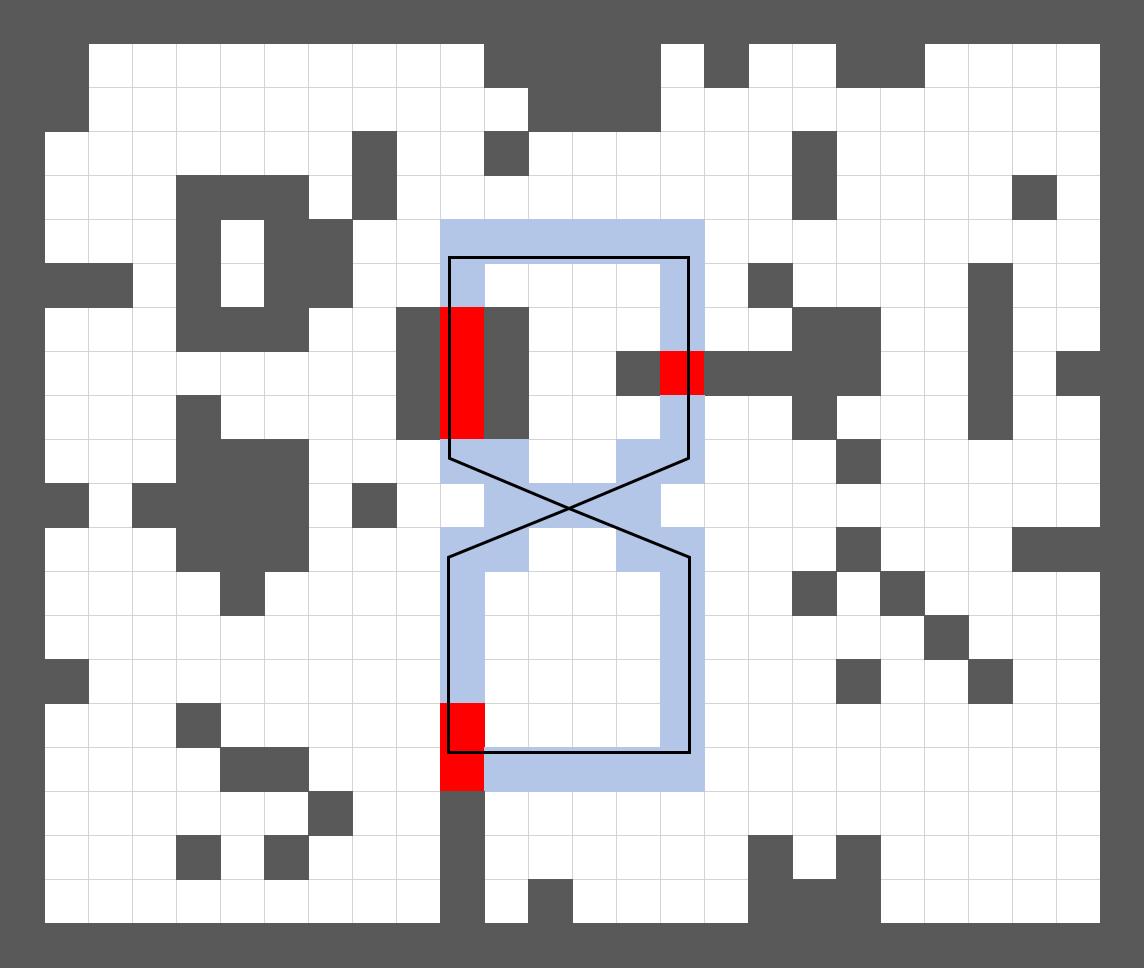
\includegraphics[width=0.4\textwidth]{bresham_colli.png}}
			\caption{铰接车在环境中的碰撞示意图}
			\label{fig:障碍物检测图}
		\end{figure}

	\section{基于NMPC和安全走廊的轨迹规划}
	在4.2节中针对铰接车对Hybrid A*算法进行了改进,它将作为轨迹规划的热启动算法。本节中将介绍如何构建一个基于NMPC的轨迹规划算法,这是一个典型的OCP最优控制框架。
		\subsection{NMPC问题构建}
		铰接式车辆运动规划的最优控制问题可以表示为其一般形式,包括成本函数以及多个等式或不等式约束。与典型的优化问题不同,基于最优控制的轨迹规划还受到一组动态微分方程的约束。一般能耗和时间最优的代价函数定义如下:
		\begin{equation}
			\begin{aligned}
				J(x(t),u(t)) &= \int_{t_0}^{t_f}
				\left\| u(t)\right\|^2dt +w_t*\left\|t_f-t_0\right\|^2    \\
				\left\|u(t)\right\|^2&=w_{uj}*\left\|jerk(t)\right\|^2+w_{uw}*\left\|\omega\right\|^2
			\end{aligned} 
		\end{equation}
		其中,$w_t$、$w_{uj}$ 和 $w_{uw}$ 分别为时间代价权重、舒适度代价权重和铰接角能耗代价权重。$\left\|u(t)\right\|^2$ 用作输入能量消耗的度量,而 $\|t_f- t_0\|^2$ 确保时间持续时间的最优性,其中 $t_f$ 和 $t_0$ 分别为结束时间和开始时间。然后这个轨迹优化问题表示为:
		\begin{equation}
			\begin{aligned}
				&\left[x^*(t),u^*(t)\right] = minimize\ J(x(t),u(t))\\      
				&s.t.\ \dot x(t)-f(x(t),u(t))=0\\
				&x_l \leq x(t) \leq x_u, u_l \leq u(t) \leq u_u,t\in \left[0,t_f\right]\\
				&x(t_0)=x_{start},x(t_f)=x_{goal}\label{eq:最优控制优化问题}
			\end{aligned}   
		\end{equation}
		其中,$\dot x(t)-f(x(t),u(t))=0$表示运动方程约束,为了保证优化问题中轨迹的平滑性。变量$x_l$和$x_u$表示状态变量的下界和上界,$u_l$和$u_u$表示控制变量的下界和上界。此外,$x_{start}$和$x_{goal}$分别对应规划问题的起点状态和终点状态。将状态方程进行离散化,求解它的最有离散子序列,即演变成一个NLP(Nonlinear Programming)问题。定义如下形式的解向量形式:
		\begin{equation}
			\begin{aligned}
				\bm{\xi} &=\left[ \bm{\xi} _{x}^{\mathrm{T}},\bm{\xi} _{y}^{\mathrm{T}},\bm{\xi} _{\theta}^{\mathrm{T}},\bm{\xi} _{\gamma}^{\mathrm{T}},\bm{\xi} _{v}^{\mathrm{T}},\bm{\xi} _{a}^{\mathrm{T}},\bm{\xi} _{\omega}^{\mathrm{T}},\bm{\xi}_{{jerk}}^{\mathrm{T}},\bm{\xi} _{\Delta t}^{\mathrm{T}} \right] ^{\mathrm{T}}\\
				\bm{\xi} _x&=\left[ x\left( 1 \right) ,...,x\left( N-2 \right) \right] ^{\mathrm{T}}\\
				\bm{\xi} _{\omega}&=\left[ \omega \left( 0 \right) ,...,\omega \left( N-2 \right) \right] ^{\mathrm{T}}
			\end{aligned}   
		\end{equation}
		其中,对于轨迹上的$N$个点,起点$P_0$和终点$P_{N-1}$是已知的。$\bm{\xi} _{x}$的维度为$n=N-2$,$\bm{\xi} _{y},\bm{\xi} _{\theta},\bm{\xi} _{\gamma},\bm{\xi} _{v},\bm{\xi} _{a}$同理。$\bm{\xi} _{\omega}$的维度为$m=N-1$,$\bm{\xi}_{jerk},\bm{\xi} _{\Delta t}$同理。

		以上所构建的优化问题中所受到的约束有状态方程约束、状态受限、输入受限、起点约束和终点约束,并没有包含避障约束。沿用安全走廊的方法,和第三章中式(\ref{eq:走廊约束})一样,避障约束是不等式的形式。假设$\bm{g}_{f}$为铰接车前桥的不等式约束函数,$\bm{g}_{r}$为铰接车后桥的不等式约束函数。则最终的轨迹规划问题可以表示为:
		\begin{equation}
			\begin{aligned}
			&J\left( \bm{\xi} \right) =w_{uj}*\lVert \bm{\xi} _{jerk} \rVert _{2}^{2}+w_{uw}*\lVert \bm{\xi} _{\omega} \rVert _{2}^{2}+w_t*\bm{I}_{N-1}^{\mathrm{T}}\bm{\xi} _{\Delta t}\\
			s.t.\ \ &\bm{g}_{kin}\left( k \right) =0,1\leq k\leq N-1\\
			&\bm{g}_{f}\left( k \right) <0,\,\,\bm{g}_{r}\left( k \right) <0,1\leq k\leq N-2\\
			&\hat{\bm{\xi}}_{min}\le \hat{\bm{\xi}}\le \hat{\bm{\xi}}_{max},\bm{\xi} _{\Delta tmin}<\bm{\xi} _{\Delta t}<\bm{\xi} _{\Delta tmax}
			\end{aligned}   
		\end{equation}
		其中,$\hat{\bm{\xi}}=\left[ \bm{\xi} _{\gamma}^{\mathrm{T}},\bm{\xi} _{v}^{\mathrm{T}},\bm{\xi} _{a}^{\mathrm{T}},\bm{\xi} _{\omega}^{\mathrm{T}},\bm{\xi} _{jerk}^{\mathrm{T}} \right] ^{\mathrm{T}}$,$\bm{g}_{kin}$是状态方程约束。方程约束中未提到的变量都是无约束变量。

		\newpage
		\vspace*{-1.5em}

		\subsection{运动学约束}
		在第二章中介绍了铰接车的运动学模型,模型的状态量为$x$、$y$、$\theta$和$\gamma$,受到微分方程的约束这些变量是天然连续的。系统的输入为速度$v$和铰接角速度$\omega$,它们并没有受到微分方程的约束,这意味着$v$和$\omega$在优化过程中直接作为优化变量是会突变的。这对于下层控制来说是不利的。为了解决这个问题,为系统引入高阶的连续性,假设系统的输入为$jerk$(加加速度或者舒适度)和$\omega$(铰接角速度)。运动学模型可以进一步写为$\dot{x}=f( x,u )$:
		\begin{equation}
			\begin{aligned}
				 \frac{\mathrm{d}}{\mathrm{d}t}\left[ \begin{array}{c}
					x\\
					y\\
					\theta\\
					\gamma\\
					v\\
					a\\
				\end{array} \right] =\left[ \begin{array}{c}
					v\cos\theta\\
					v\sin\theta\\
					v\tan( \gamma /2 ) /L+\omega / (\cos\gamma +1 )\\
					\omega\\
					a\\
					jerk\\
				\end{array} \right] 
			\end{aligned}   
		\end{equation}
		其中, 令$\bm{x}=\left[ x,y,\theta,\gamma,v,a \right]^{\mathrm{T}}$ 为状态向量,分别表示前轴中点位置、航向角、铰接角、速度、加速度。输入向量由 $\bm{u}=\left[jerk,\omega\right]^{\mathrm{T}}$ 给出,其中 $jerk$ 为前轴中点加加速度(舒适度),$\omega$ 为铰接角速度。

		对于上述运动学方程需要对其进行离散化,采用一阶离散运动学模型,可表示为:
		\begin{equation}
			\begin{aligned}
				\bm{x}( k ) =\bm{x}( k-1 ) +\Delta t( k-1 ) f( \bm{x}( k-1 ) ,\bm{u}( k-1 ) ) 
			\end{aligned}   
		\end{equation}

		令 $\bm{g}_{kin} = [\bm{g}_x^{\mathrm{T}}\ \bm{g}_y^{\mathrm{T}}\ \bm{g}_\theta^{\mathrm{T}}\ \bm{g}_\gamma^{\mathrm{T}}\ \bm{g}_v^{\mathrm{T}}\ \bm{g}_a^{\mathrm{T}}]^{\mathrm{T}}$,其中 $\bm{g}_{kin}$的每一个元素对应 $m = N-1$ 个等式约束。例如:
		\begin{equation}
			\begin{aligned}
				g_{x}( 0 ) =x_f( 1 ) -x_{start}-\Delta t( 0 ) \cdot v( 0 ) \cos \theta( 0 ) \\
				g_{x}( 1 ) =x_f( 2 ) -x_f( 1 ) -\Delta t( 1 ) \cdot v( 1 ) \cos \theta ( 1 ) \\
				...\\
				g_{y}( 0 ) =y_f( 1 ) -x_{start}-\Delta t( 0 ) \cdot v( 0 ) \sin \theta ( 0 ) \\
				g_{y}( 1 ) =y_f( 2 ) -y_f( 1 ) -\Delta t( 1 ) \cdot v( 1 ) \sin \theta ( 1 ) \\
				...
			\end{aligned}   
		\end{equation}

		使用惩罚函数将运动学约束纳入代价函数,表达式如下:
		\begin{equation}
			\mathcal{G}_{kin} = w_{kin}*\left \| \bm{g}_{kin} \right \|_2^2 \label{Gkin}
		\end{equation}
		梯度为:
		\begin{equation}
			\frac{\partial\mathcal{G}_{kin}}{\partial\bm{\xi}}=2w_{kin}\cdot\frac{\partial \bm{g}_{kin}^{\mathrm{T}}}{\partial\bm{\xi}}\cdot \bm{g}_{kin}\label{18}
		\end{equation}
		其中,$w_{kin}$为运动学约束权重。\(\frac{\partial \bm{g}_{kin}^{\mathrm{T}}}{\partial \bm{\xi}}\) 表示所有运动约束向量的雅可比矩阵,表示为:
		\begin{equation}
			\begin{array}{c}
				\frac{\partial \bm{g}_{kin}^{\mathrm{T}}}{\partial \bm{\xi}}= 
				{\left[\begin{array}{cccccc}
						\bm{\psi}_{E} & 0 & 0 & 0 & 0 & 0 \\
						0 & \bm{\psi}_{E} & 0 & 0 & 0 & 0 \\
						-\bm{\psi}_{x \theta} & -\bm{\psi}_{y \theta} & \bm{\psi}_{E} & 0 & 0 & 0 \\
						0 & 0 & -\bm{\psi}_{\theta \gamma} & \bm{\psi}_{E} & 0 & 0 \\
						-\bm{\psi}_{x v} & -\bm{\psi}_{y v} & -\bm{\psi}_{\theta v} & 0 & \bm{\psi}_{E} & 0 \\
						0 & 0 & 0 & 0 & -\bm{\psi}_{v a} & \bm{\psi}_{E} \\
						0 & 0 & -\bm{\psi}_{\theta \omega} & -\bm{\psi}_{\gamma \omega} & 0 & 0 \\
						0 & 0 & 0 & 0 & 0 & -\bm{\psi}_{\text {ajerk }} \\
						-\bm{\psi}_{x \Delta t} & -\bm{\psi}_{y \Delta t} & -\bm{\psi}_{\theta \Delta t} & -\bm{\psi}_{\gamma \Delta t} & -\bm{\psi}_{v \Delta t} & -\bm{\psi}_{a \Delta t}
					\end{array}\right]}
			\end{array}
			\label{eq:运动学约束的雅可比}
		\end{equation}
		其中, $\bm{\psi}_E = [\bm{E}_{n \times n}, 0_n] - [0_n, \bm{E}_{n \times n}]$,其中 $\bm{E}$ 为单位矩阵,且\(\bm{\psi}_{ij} = \frac{\partial \bm{g}^{\mathrm{T}}_{i}}{\partial \bm{\xi}_j}\)。

		\subsection{安全走廊的防碰撞约束处理}
		在本节中,将探讨避障约束在笛卡尔坐标系中的表述方法。仍然采用安全走廊对铰接车的避障进行全维建模,安全走廊的构建方法参照第三章中的全局规划方案。与全局规划中的处理方式不同,本节中将对车体结构进行建模。在全局规划中,车体被简化为质点模型,且车体结构的影响通过膨胀层来近似替代,其主要目的是快速生成一条长远的路径,以为局部规划提供导航指引。而局部规划则负责生成更加精细化的轨迹。

		如图\ref{fig:安全走廊}所示,灰色区域是设置的障碍物示意,黑色的是运动轨迹。轨迹上设置有多个离散点,蓝色的区域是凸多边形安全区域。每一个离散的路径点都生成一个凸多边形,这些凸多边形依次相交形成安全走廊,所有优化轨迹点都将被约束在该走廊内。

		\newpage
		\vspace*{-1.5em}

		\begin{figure}[H]
			\centering
			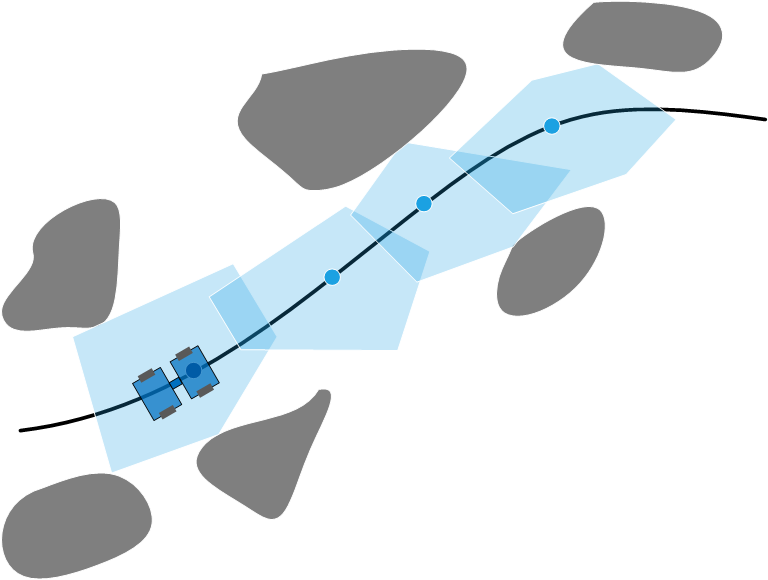
\includegraphics[width=0.9\textwidth]{安全走廊.png}
			\caption{安全走廊示意图}
			\label{fig:安全走廊}
		\end{figure}

		铰接车辆的前桥由四个顶点构成,这四个顶点围成一个凸多边形,即为前桥的轮廓。同样地,后桥也具有类似的四个顶点,形成其自身的凸多边形轮廓。基于凸集的性质,如果将车辆的所有顶点都包含在一个大的凸包内,则可以确定整个车辆都将位于这个凸包之内。例如,在判断车辆是否能够安全通过狭窄通道或避开障碍物时,可以通过检查车辆的凸包是否与障碍物或其他限制发生重叠来进行决策。进一步,考虑到铰接式车辆在转向过程中前后桥的相对位置会发生变化,采用动态更新的凸包能更准确地反映车辆的实际形态和运动轨迹。可以得到如下安全约束:
		\begin{equation}
			\left\{ \begin{matrix}
				\bm{A}\left( \bm{R}_{\theta}\bm{l}_f+\bm{\sigma} \right) -\bm{b}<0,&		f=A,B,C,D\\
				\bm{A}\left( \bm{R}_{\gamma}\bm{R}_{\theta}\bm{l}_r+\bm{R}_{\theta}\bm{l}_{O_1}+\bm{\sigma} \right) -\bm{b}<0,&		r=E,F,G,H\\
			\end{matrix} \right. 
		\end{equation}

		由于铰接角的运动范围有限,仅利用前轴的四个顶点很多时候就足以实现有效的避障。
		为了方便表达,令
		\begin{equation}
			\begin{aligned}
			\bm{g}_{f}\left( \bm{\sigma} ,\theta ,\gamma \right) &=\bm{A}\left( \bm{R}_{\theta}\bm{l}_f+\bm{\sigma} \right) -b\\
			\bm{g}_r\left( \bm{\sigma} ,\theta ,\gamma \right) &=\bm{A}\left( \bm{R}_{\gamma}\bm{R}_{\theta}\bm{l}_r+\bm{R}_{\theta}\bm{l}_{O_1}+\bm{\sigma} \right) -b
			\end{aligned}
		\end{equation}
		其中,$\bm{R}_{\theta +\gamma}=\bm{R}_{\theta}\bm{R}_{\gamma},\ \bm{R}_{\theta}=\left[ \begin{matrix}
			\cos\theta&		-\sin\theta\\
			\sin\theta&		\cos\theta\\
		\end{matrix} \right] $。
		路径上第$k$个点处的走廊约束关于$\bm{\sigma}_k,\theta_k$和$\gamma_k$的梯度由下式给出:
		\begin{equation}
			\begin{aligned}
			\frac{\partial \bm{g}_{f}^{\mathrm{T}}(k)}{\partial \bm{\sigma} _k}&=\bm{A}_{k}^{\mathrm{T}},\frac{\partial \bm{g}_{f}^{\mathrm{T}}(k)}{\partial \gamma _k}=0,\frac{\partial \bm{g}_{f}^{\mathrm{T}}(k)}{\partial \theta _k}=\bm{l}_{f}^{\mathrm{T}}\frac{\partial \bm{R}_{\theta}^{\mathrm{T}}}{\partial \theta _k}\bm{A}_{k}^{\mathrm{T}}\\
			\frac{\partial \bm{g}_{r}^{\mathrm{T}}(k)}{\partial \bm{\sigma} _k}&=\bm{A}_{k}^{\mathrm{T}},\frac{\partial \bm{g}_{r}^{\mathrm{T}}(k)}{\partial \gamma _k}=\bm{l}_{r}^{\mathrm{T}}\frac{\partial \bm{R}_{\theta +\gamma}^{\mathrm{T}}}{\partial \gamma _k}\bm{A}_{k}^{\mathrm{T}}\\
			\frac{\partial \bm{g}_{r}^{\mathrm{T}}(k)}{\partial \theta _k}&=\bm{l}_{r}^{\mathrm{T}}\frac{\partial \bm{R}_{\theta +\gamma}^{\mathrm{T}}}{\partial \theta _k}\bm{A}_{k}^{\mathrm{T}}+\bm{l}_{o1}^{\mathrm{T}}\frac{\partial \bm{R}_{\theta}^{\mathrm{T}}}{\partial \theta _k}\bm{A}_{k}^{\mathrm{T}}
			\end{aligned}
		\end{equation}

		对于上述走廊的不等式约束,使用罚函数将约束加入到代价函数中。为了确保连续可微性,罚函数使用式(\ref{eq:松弛函数})。为了方便表达,定义 \([]\) 为逐元素运算符,例如 \([\cdot]\) 表示逐元素乘法,\(S[x]\) 表示对$x$的所有元素进行函数 \(S\)运算。于是可以得到总体的走廊约束代价,其表达为:
		\begin{equation}
			\mathcal{G}_c =\mathcal{G}_{f}+\mathcal{G}_{r}=w_{c}\cdot \sum_{k=1}^{N-2}\sum_{i=0}^{d-1}(S[\bm{g}_{f}(k)] + S[\bm{g}_{r}(k)])\label{eq:走廊约束代价}
		\end{equation}
		其中,$d$为矩阵$\bm{A}_k$的行数。对式(\ref{eq:走廊约束代价})中的各项分别进行求导得到走廊的惩罚项的梯度:
		\begin{equation}
			\begin{aligned}
				\frac{\partial \mathcal{G}_{f,r}}{\bm{\sigma} \left( k \right)}&=\sum_{i=0}^{d-1}{\bm{A}}_{k}^{\mathrm{T}}S^{'}\left[ \bm{g}_{f,r}\left( k \right) \right] =\bm{A}_{k}^{\mathrm{T}}S^{'}\left[ \bm{g}_{f,r}\left( k \right) \right] \bm{I}_d\\
				\frac{\partial \mathcal{G}_f}{\bm{\xi} _{\theta}\left( k \right)}&=\bm{l}_{f}^{\mathrm{T}}\frac{\partial \bm{R}_{\theta}^{\mathrm{T}}\left( k \right)}{\partial \theta \left( k \right)}\bm{A}_{k}^{\mathrm{T}}S^{'}\left[ \bm{g}_{f}\left( k \right) \right] \bm{I}_d\\
				\frac{\partial \mathcal{G}_r}{\bm{\xi} _{\gamma}\left( k \right)}&=\bm{l}_{r}^{\mathrm{T}}\frac{\partial \bm{R}_{\theta +\gamma}^{\mathrm{T}}\left( k \right)}{\partial \gamma \left( k \right)}\bm{A}_{k}^{\mathrm{T}}S^{'}\left[ \bm{g}_{r}\left( k \right) \right] \bm{I}_d\\
				\frac{\partial \mathcal{G}_r}{\bm{\xi} _{\theta}\left( k \right)}&=\left( \bm{l}_{r}^{\mathrm{T}}\frac{\partial \bm{R}_{\theta +\gamma}^{\mathrm{T}}\left( k \right)}{\partial \theta \left( k \right)}+\bm{l}_{o1}^{\mathrm{T}}\frac{\partial \bm{R}_{\theta}^{\mathrm{T}}\left( k \right)}{\partial \theta \left( k \right)} \right) \bm{A}_{k}^{\mathrm{T}}S^{'}\left[ \bm{g}_{r}\left( k \right) \right] \bm{I}_d\\
				\bm{\sigma} \left( k \right) &=\left[ \bm{\xi} _x\left( k \right) ,\bm{\xi} _y\left( k \right) \right] ^{\mathrm{T}}
			\end{aligned}
		\end{equation}
		
		\subsection{变量的边界约束}
		在实际的系统中,系统的输入和状态不是无边界的,例如铰接车的速度、加速度、加加速度、铰接角等变量,所以需要对这些变量进行约束分析。由于边界约束同样和走廊约束一样是不等式约束,采用走廊约束处理方法,使用松弛函数$S(\cdot)$加入到代价函数中。为了表示方便后序将省略下标,变量边界约束对应的罚函数项和其梯度如下:
		\begin{equation}
			\begin{aligned}
				\mathcal{G}_b&=w_b\cdot \sum_{k=0}^{cols}{\left( S\left[ \hat{\bm{\xi}}_{min}-\hat{\bm{\xi}} \right] +S\left[ \hat{\bm{\xi}}-\hat{\bm{\xi}}_{max} \right] \right)}\\
				&=w_b\cdot \bm{I}_{N-2}^{\mathrm{T}}\left( S\left[ \hat{\bm{\xi}}_{min}-\hat{\bm{\xi}} \right] +S\left[ \hat{\bm{\xi}}-\hat{\bm{\xi}}_{max} \right] \right)\\
				\frac{\partial \mathcal{G}_b}{\hat{\bm{\xi}}}&=w_b\cdot \left( S^{'}\left[ \hat{\bm{\xi}}-\hat{\bm{\xi}}_{max} \right] -S^{'}\left[ \hat{\bm{\xi}}_{min}-\hat{\bm{\xi}} \right] \right)
			\end{aligned}
			\label{eq:Gb}
		\end{equation}
		其中,$w_b$是边界约束的权重,$\bm{I}_{N-2}$表示元素全为1的$N$-2维向量。

		\subsection{时间正则化约束}
		在本文的轨迹优化问题中,每两个轨迹点之间的时间$\Delta t$是灵活变化且独立的,纳入了优化变量当中。时间正则化约束和走廊约束一样属于不等式约束,与之不同的是,时间项$\Delta t$必须严格大于0,这是硬约束。使用松弛函数对时间项进行惩罚属于约束软化的过程,在极端的场景下仍然可能出现$\Delta t \le 0$,这并不符合物理规律。

		为了解决以上问题,本文使用一个sigmoid变换将$\Delta t$的取值范围区间映射到映射到负无穷到正无穷,变换后的变量记为$\tau$。这个变换是微分同胚的,微分同胚变换前后不会为优化问题引入额外的极小值\upcite{wang2022geometrically}。
		\begin{equation}
			\begin{aligned}
				\Delta t\left( \tau \right) =\frac{\Delta t_{max}}{1+e^{-\frac{\tau}{\Delta t_{max}}}},\,\,\,\,\Delta t^{'}\left( \tau \right) =\frac{e^{-\frac{\tau}{\Delta t_{max}}}}{\left( 1+e^{-\frac{\tau}{\Delta t_{max}}} \right) ^2}
			\end{aligned}
		\end{equation}
		其中,$t_{max}$为时间变量的上界。$-\infty <\tau <+\infty $,$0<\Delta t<\Delta t_{max}$。
		
		\subsection{优化问题求解}
		在上面几个小节,利用惩罚函数来表示成本函数中的运动学约束,并使用松弛函数来表示成本函数中的走廊约束,对于时间变量被映射到了整个实数轴,最后所有约束都被处理,问题被化为一个无约束优化的形式

		由于时间变量用微分同胚进行了转换,需要重新表示优化变量。令最终的优化变量$\eta =\left[ \bm{\xi} _{x}^{\mathrm{T}},\bm{\xi} _{y}^{\mathrm{T}},\bm{\xi} _{\theta}^{\mathrm{T}},\bm{\xi} _{\gamma}^{\mathrm{T}},\bm{\xi} _{v}^{\mathrm{T}},\bm{\xi} _{a}^{\mathrm{T}},\bm{\xi} _{\omega}^{\mathrm{T}},\bm{\xi} _{jerk}^{\mathrm{T}},\bm{\xi} _{\tau}^{\mathrm{T}} \right] ^{\mathrm{T}}$,在这里$\bm{\xi} _{\tau}$和最初优化变量$\bm{\xi}$中的$\bm{\xi} _{t}$是微分同胚的。于是代价函数可以重新写为:
		\begin{equation}
			\begin{aligned}
				\mathcal{J}\left( \eta \right) =J\left( \bm{\xi} \right) +\mathcal{G}_{kin}+\mathcal{G}_c+\mathcal{G}_b
			\end{aligned}
		\end{equation}
		其中,$J(\bm{\xi})$对应的梯度为:
		\begin{equation}
			\begin{aligned}
				\frac{\partial J}{\partial \bm{\xi} _{jerk}}&=2w_{uj}\cdot \bm{\xi} _{jerk}\\
				\frac{\partial J}{\partial \bm{\xi} _{\omega}}&=2w_{u\omega}\cdot \bm{\xi} _{\omega}\\
				\frac{\partial J}{\partial \bm{\xi} _{\tau}}&=w_t\cdot diag(\Delta t^{'}\left[ \bm{\xi} _{\tau} \right])I_{N-1}
			\end{aligned}
		\end{equation}
		其中,$diag(\Delta t^{'}\left[ \bm{\xi} _{\tau} \right])$表示以$\Delta t^{'}\left[ \bm{\xi} _{\tau} \right]$为对角线元素的对角阵。在式(\ref{eq:走廊约束代价})推导出了运动学约束的雅可比矩阵。现在把对时间变量的导数部分进行替换,得到:
		\begin{equation}
			\begin{aligned}
				\bm{\psi} _{i\tau}=\frac{\partial \bm{g}_{i}^{\mathrm{T}}}{\partial \bm{\xi} _{\tau}}=diag(\Delta t^{'}\left[ \bm{\xi} _{\tau} \right])\cdot \frac{\partial \bm{g}_{i}^{\mathrm{T}}}{\partial \bm{\xi} _{\Delta t}}
			\end{aligned}
		\end{equation}
		其中,$\mathcal{G}_{kin},\mathcal{G}_c,\mathcal{G}_b$由式(\ref{Gkin})、式(\ref{eq:走廊约束代价})和式(\ref{eq:Gb})提供。
		综上所述,优化问题被转化为了一个无约束的形式,可以使用L-BFGS算法求解。

	\section{本章小结}
	在本章中,提出了一种基于安全走廊的铰接车局部轨迹规划方法,并通过最优控制框架对其进行建模与求解。首先,对铰接车的外观进行了通用性的建模,并通过简化车辆形状为两个矩形的连接,转化了避障问题为几何碰撞问题。其次,提出了针对铰接车的Hybrid A*算法改进,通过调整节点拓展策略并结合铰接车的运动学特性,优化了路径规划的效率与准确性。

	在轨迹优化方面,构建了基于NMPC的轨迹规划方法,定义了优化问题并加入了动力学约束、运动学约束及避障约束。通过引入适合铰接车的运动学模型和代价函数,确保了在求解过程中能够考虑车辆的舒适度与能效,同时解决了车辆输入突变的问题。
	% 下面给出局部规划算法的伪代码:
	% \begin{algorithm}[H]  
	% 	\caption{Local Planning}  
	% 	\label{alg:local_planning}  
	% 	\begin{algorithmic}[1]  
	% 		\REQUIRE  
	% 		$\bm{p}_{start},\bm{p}_{end},\bm{map}$
	% 		\ENSURE  
	% 		$\bm{traj}^{opt}$
	% 		\STATE $\bm{traj}^{coarse} \leftarrow HybridAstar(\bm{p}_{start},\bm{p}_{end},\bm{map})$\\
	% 		\STATE $\bm{\xi}_0 \leftarrow getGuess(\bm{traj}^{coarse})$\\
	% 		\STATE $cors \leftarrow getCorridor(\bm{map},\bm{traj}^{coarse})$\\
	% 		\STATE $cons \leftarrow getConstraint(\bm{\xi}_{min,max},cors,kinEqn)$\\
	% 		\STATE $cosFcn \leftarrow getCost(cons)$\\
	% 		\STATE $grad \leftarrow getGrad(cons)$ \\
	% 	   \RETURN $\bm{traj}^{opt} \leftarrow \bm{lbfgs}(cosFcn,grad)$
	% 	\end{algorithmic}  
	% \end{algorithm}

	通过本章的研究,不仅改进了传统轨迹规划算法以适应铰接车的特殊运动特性,还设计了高效的碰撞检测与轨迹优化方案,为铰接车在复杂环境中的局部路径规划提供了有效的解决方案。
	
	\chapter{铰接车运动规划系统仿真}
	第三章和第四章分别介绍了全局轨迹规划和局部轨迹规划算法,并对两者的理论基础进行了分析。本章将这两个算法集成到ROS仿真系统中,通过大量仿真场景验证算法性能,进而展示算法整体的规划能力。
	
	表\ref{tab:仿真车体参数}给出了车体的仿真参数设置,仿真中都将使用栅格地图最为环境信息,地图的的分辨率是0.3 m/pix。
	\begin{table}[!ht]
		\caption{仿真车体参数表}
		\label{tab:仿真车体参数}
		\centering
		\begin{tabular}{CLR}
			\toprule
			参数 & 描述 & 数值 \\
			\midrule
			$L$ &前轴/后轴长度 &1.3 m\\			
			$L_1$ &前桥长度  &1.8 m\\			
			$L_2$ & 后桥长度 &1.8 m\\			
			$d$   &半轮轴长度  &1.8 m\\		
			$d_1$ &前轮轴到A点的距离 &1.075 m\\			
			$d_2$ &后轮轴到H点的距离  &1.075 m\\			
			$width$ &前桥宽度(BC)  &2.1 m\\			
			$v_{min}$ &车体速度下界 &-3 m/s\\			
			$v_{max}$ &车体速度上界  &3 m\\			
			$a_{min}$ &车体加速度下界 &-2 m/s$^\text{2}$\\			
			$a_{max}$ &车体加速度上界 &2 m/s$^\text{2}$\\			
			$jerk_{min}$ &车体加加速度下界      &-3 m/s$^\text{3}$\\			
			$jerk_{max}$ &车体加加速度上界     &3 m/s$^\text{3}$\\
			$\gamma_{min}$ &铰接角下界 &-0.52 rad\\
			$\gamma_{max}$ &铰接角上届 &0.52 rad\\
			$\omega_{min}$ &铰接角速度下界 &-0.2 rad/s\\
			$\omega_{max}$ &铰接角速度上界 &0.2 rad/s\\
			\bottomrule
		\end{tabular}
	\end{table}

	\section{仿真环境及运动规划软件架构设计}
	本文仿真环境搭载AMD-Ryzen9-7940HX处理器,基于Ubuntu20.04LTS操作系统构建ROS-Noetic机器人系统框架。仿真可视化界面使用RVIZ,其仿真界面示意见图\ref{fig:rviz仿真界面}。核心算法采用C++14标准和Eigen矩阵库实现,并通过Catkin构建系统实现节点编译与依赖管理。
	\begin{figure}[H]
		\centering
		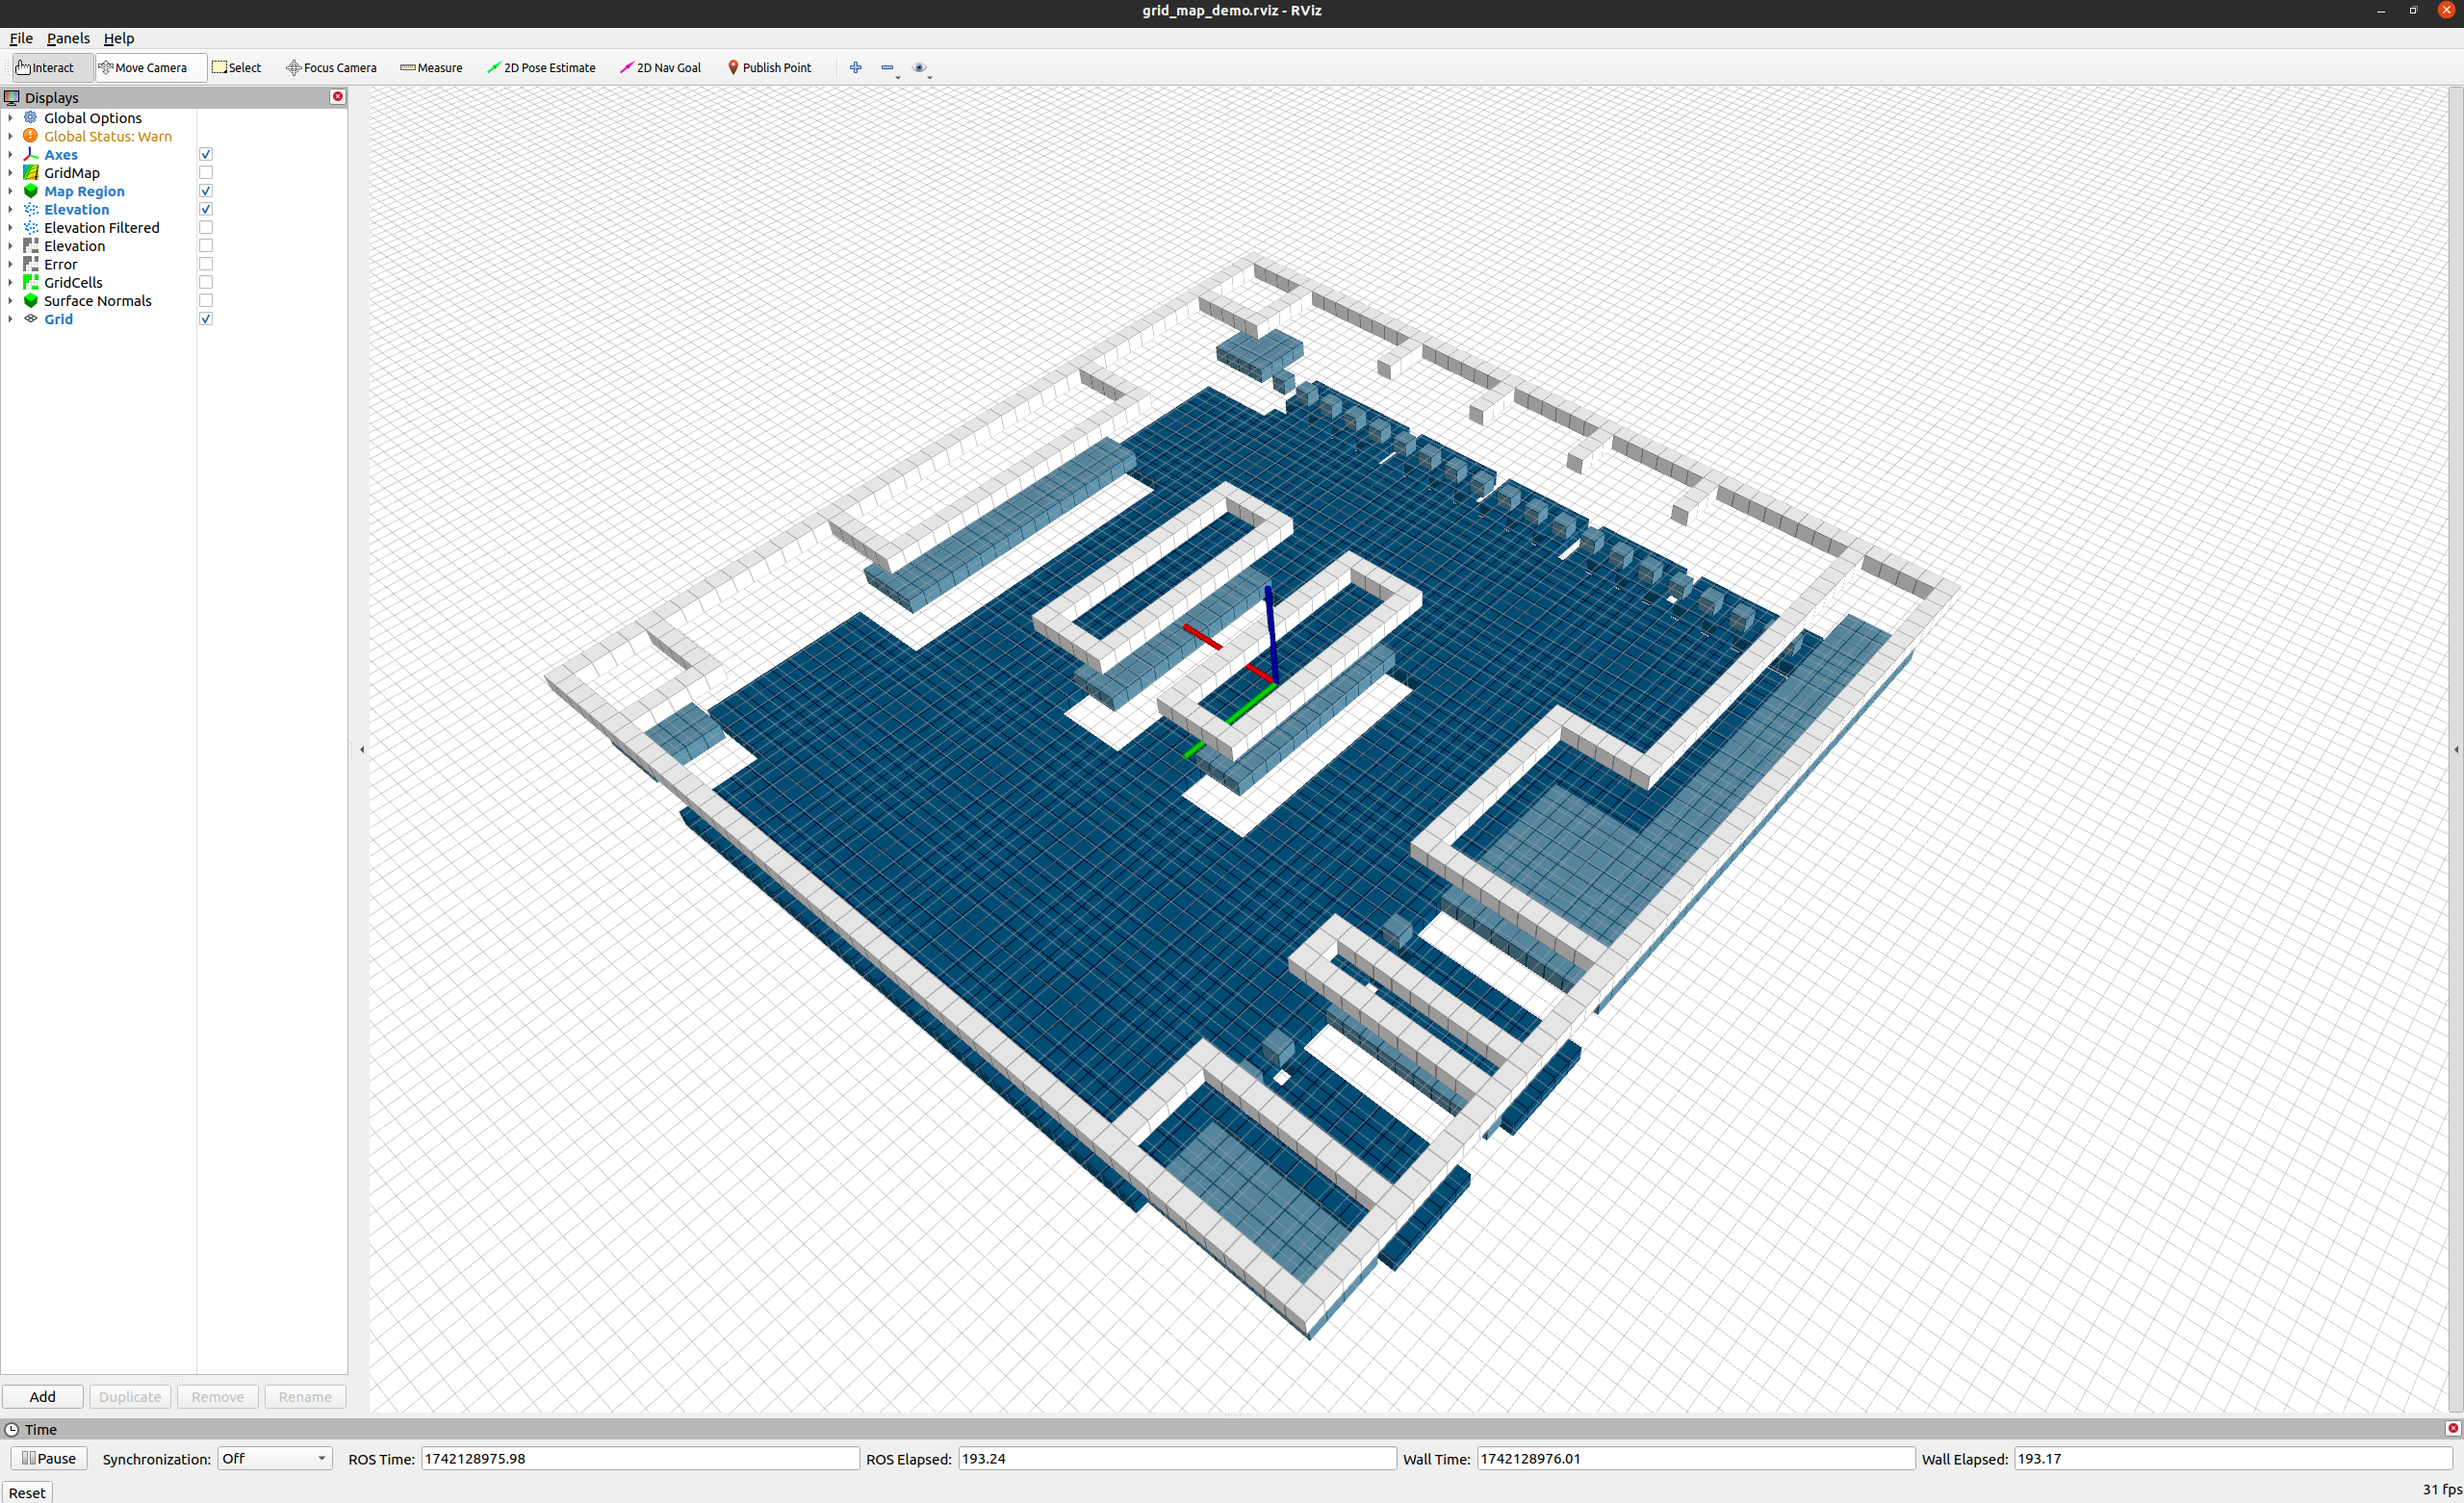
\includegraphics[width=0.75\textwidth]{rviz_view.png}
		\caption{RVIZ仿真可视化示意}
		\label{fig:rviz仿真界面}
	\end{figure}

	受开源机器人框架ROS的启发,本文的运动规划系统采用全局-局部双级递进架构实现任务分解。图\ref{fig:运动规划算法框架}为运动规划系统的算法架构:
		\begin{figure}[H]
			\centering
			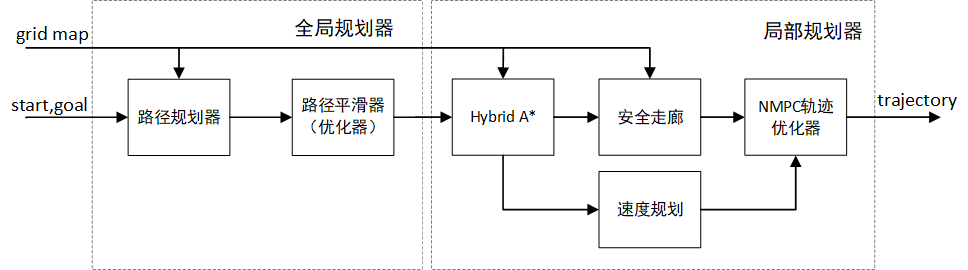
\includegraphics[width=1.0\textwidth]{运动规划算法框架.png}
			\caption{运动规划算法架构}
			\label{fig:运动规划算法框架}
		\end{figure}

	在ROS中,navigation框架以move\_base节点作为整个机器人的运动逻辑控制中心,集成了定位、路径规划、避障和运动控制等关键功能。它通过自适应蒙特卡洛定位(​AMCL)算法实现机器人在已知地图中的实时定位,利用全局规划器生成最优路径,并通过局部规划器实时调整路径以避开动态障碍物。全局代价地图和局部代价地图更新环境信息,确保导航安全。支持灵活配置传感器、规划算法及地图参数,适用于服务机器人、仓储物流和工业自动化等场景,提供从建图到自主导航的一体化解决方案。但是目前正处于机器人高速发展的时期,navigation会随着ROS版本的更替而快速更替,这给开发者带来了很多的不便。而move\_base\_flex的诞生解决了这个问题,该框架以向后兼容为目的,旨在让使用者可以不必关注于框架的改变,可以快速适配自己的机器人。图\ref{fig:navigation规划框架图}为navigation的规划软件架构。如图\ref{fig:改进的规划框架图}是本文改进的规划框架图。
	\begin{figure}[H]
		\centering
		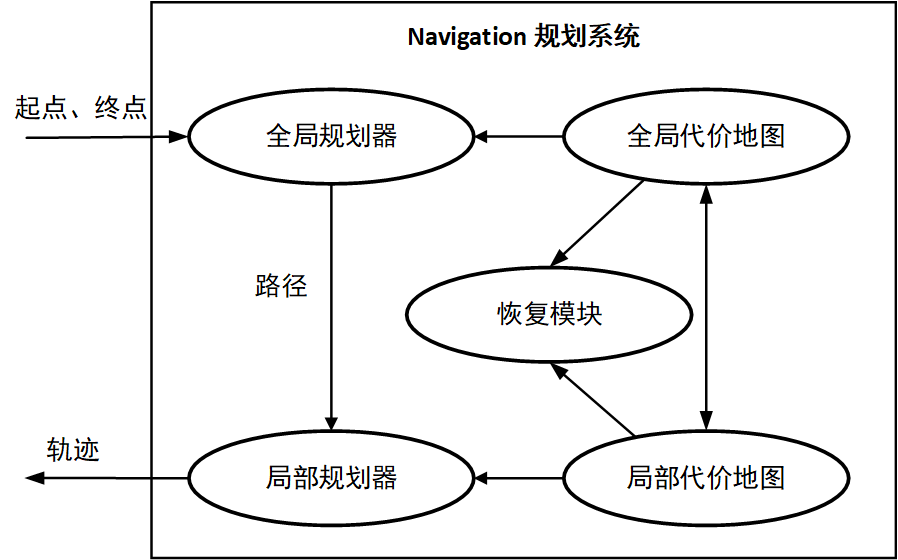
\includegraphics[width=0.8\textwidth]{navigation规划框架.png}
		\caption{navigation规划软件架构图}
		\label{fig:navigation规划框架图}
	\end{figure}
	\begin{figure}[H]
		\centering
		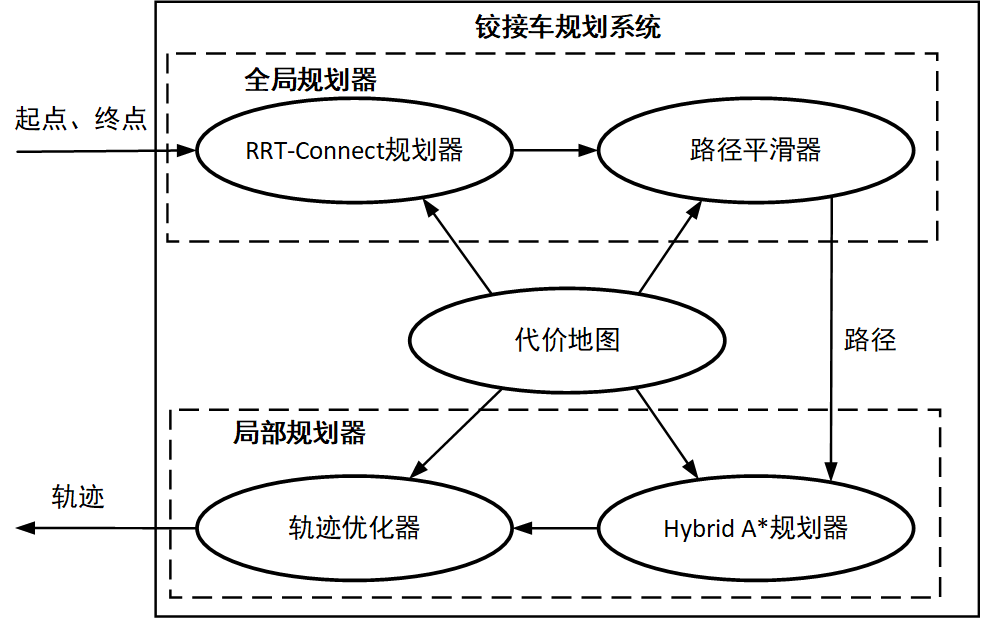
\includegraphics[width=0.8\textwidth]{我的规划框架.png}
		\caption{改进的铰接车软件架构图}
		\label{fig:改进的规划框架图}
	\end{figure}
	
	在ROS中navigation规划框架由全局规划器、局部规划器、全局代价代价地图和局部代价地图构成。全局规划器利用全局代价地图提供的环境信息使用A*或者Dijkstra算法完成路径规划。局部规划器使用局部代价地图提供的环境信息,使用DWA(Dynamic Window Approach)和TEB(Timed Elastic Band)算法进行局部轨迹规划。图\ref{fig:URDF铰接式底盘模型}为仿真使用到的URDF铰接式仿真模型。
	\begin{figure}[H]
		\centering
		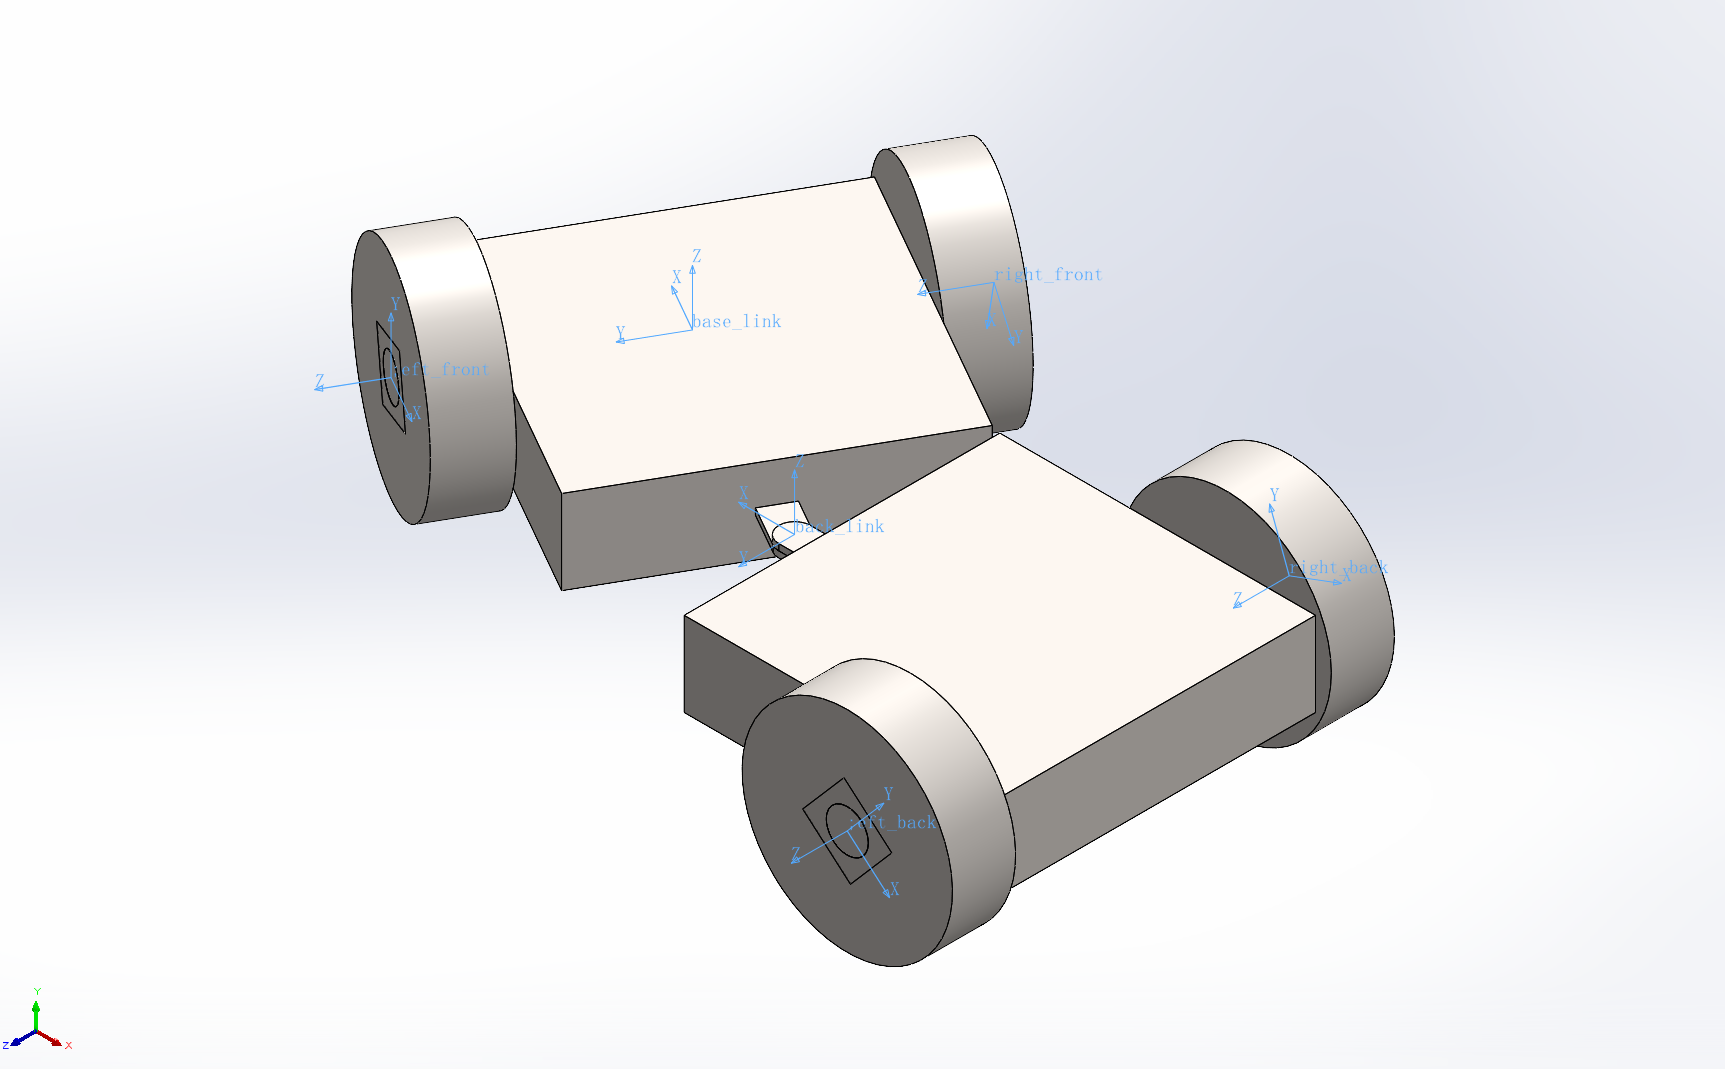
\includegraphics[width=0.8\textwidth]{urdf.png}
		\caption{URDF铰接式底盘模型}
		\label{fig:URDF铰接式底盘模型}
	\end{figure}
	
	相较于navigation的规划架构本文做了几个变化:

	首先,移除了恢复模块。在标准的navigation系统中,恢复模块的主要功能是在机器人遇到困境时(例如陷入狭窄空间或被障碍物包围),提供必要的恢复行为,帮助机器人脱离困境。然而,在本文的仿真环境中,由于地图是预先设定且静态不变的,并没有动态变化的情况,因此恢复模块是没必要的。通过去除这一模块,不仅简化了系统的复杂性,还提高了整体框架的效率和稳定性。

	其次,合并全局代价地图与局部代价地图。通常情况下,全局和局部规划器需要实时更新环境中的静态和动态障碍物信息,这对计算资源提出了挑战。为了应对这个问题,navigation系统设计了独立工作的全局和局部代价地图,以确保系统能够高效运行。但在本文的仿真场景中,由于所有障碍物都是事先加载且固定不变的,不存在动态障碍物的情况。因此将这两个代价地图合并以提升了系统的响应速度和性能表现。

	进一步,对全局规划器进行了重构,将其分为RRT-Connect规划器和路径平滑器两个主要部分。RRT-Connect专注于前端快速路径搜索,能够在短时间内找到一条从起点到终点的基本可行路径;而路径平滑器则负责后端处理,对这条路径进行平滑处理,并根据具体需求施加曲率限制,确保生成的路径既安全又符合机器人的运动特性。这两者紧密结合,共同构成了一个高效的全局轨迹规划方案。

	最后,对局部规划器进行了重构。新的局部规划器由Hybrid A*规划器和轨迹优化器组成。Hybrid A*用于前端快速搜索允许倒车的轨迹,它能在复杂的环境中迅速找到一条初步可行的轨迹;随后,轨迹优化器对这条路径进行进一步优化,确保其满足一系列约束条件,包括运动学约束、安全性要求以及边界限制等。
	
	% 这样的设计使得局部规划器不仅能适应更广泛的应用场景,还能提高机器人执行任务的成功率和安全性。

	\section{全局规划算法仿真}
	在本节中,将对全局规划算法进行仿真测试。该算法的理论原理已在第三章中详细推导和分析。为了验证提出的算法的有效性,本文分别在单点到点导航场景和多点导航场景下进行全局规划测试。在这两种仿真场景中,所使用的权重参数保持一致,具体参数值见表 \ref{tab:全局规划仿真参数}。
	\begin{table}[!ht]
		\caption{全局规划仿真参数}
		\label{tab:全局规划仿真参数}
		\centering
		\begin{tabular}{CLR}
			\toprule
			参数 & 描述 & 数值 \\
			\midrule
			$k_{min}$ &最小曲率 &-0.1\\
			$k_{max}$ &最大曲率 &0.1\\
			$w_{k}$ &曲率约束惩罚权重 &100\\
			$w_c$ &走廊约束惩罚权重 &10\\
			\bottomrule
		\end{tabular}
	\end{table}
	
	表 \ref{tab:全局规划仿真参数} 中仿真设定的最大曲率为0.1,最小曲率为-0.1。实际上,本文的铰接车辆允许的最大曲率为0.2,为了给后续的局部轨迹优化留出一定的裕量,设置了较为保守的曲率限制。由于Minco样条基于五次多项式,其对自变量的数值变化较为敏感,尤其在接近航点时易产生振荡,从而导致轨迹违反曲率约束。因此,曲率约束权重$w_k$的选取应以走廊约束权重$w_c$为基准,并提高一个数量级以上。

		\subsection{点到点路径规划仿真}
		本小节的主要目的是通过仿真验证第三章中点到点场景下的路径规划任务,展示规划算法在穿越不同障碍物下的表现,并评估其生成路径的质量和效率。
		
		图 \ref{fig:点到点路径规划仿真案例} 是点到点规划的仿真结果图,其中图\ref{fig:点到点路径规划仿真案例}\subref{fig:single_3}和\ref{fig:点到点路径规划仿真案例}\subref{fig:single_4}分别是在不同起点和终点下的规划结果。图 \ref{fig:single} 单独展示了一个路径规划仿真例子,用于对局部路径规划算法进行定性分析。

		\newpage
		\vspace*{-1.5em}

		\begin{figure}[H]
			\centering
			\subcaptionbox{示意一\label{fig:single_3}}[0.49\textwidth]{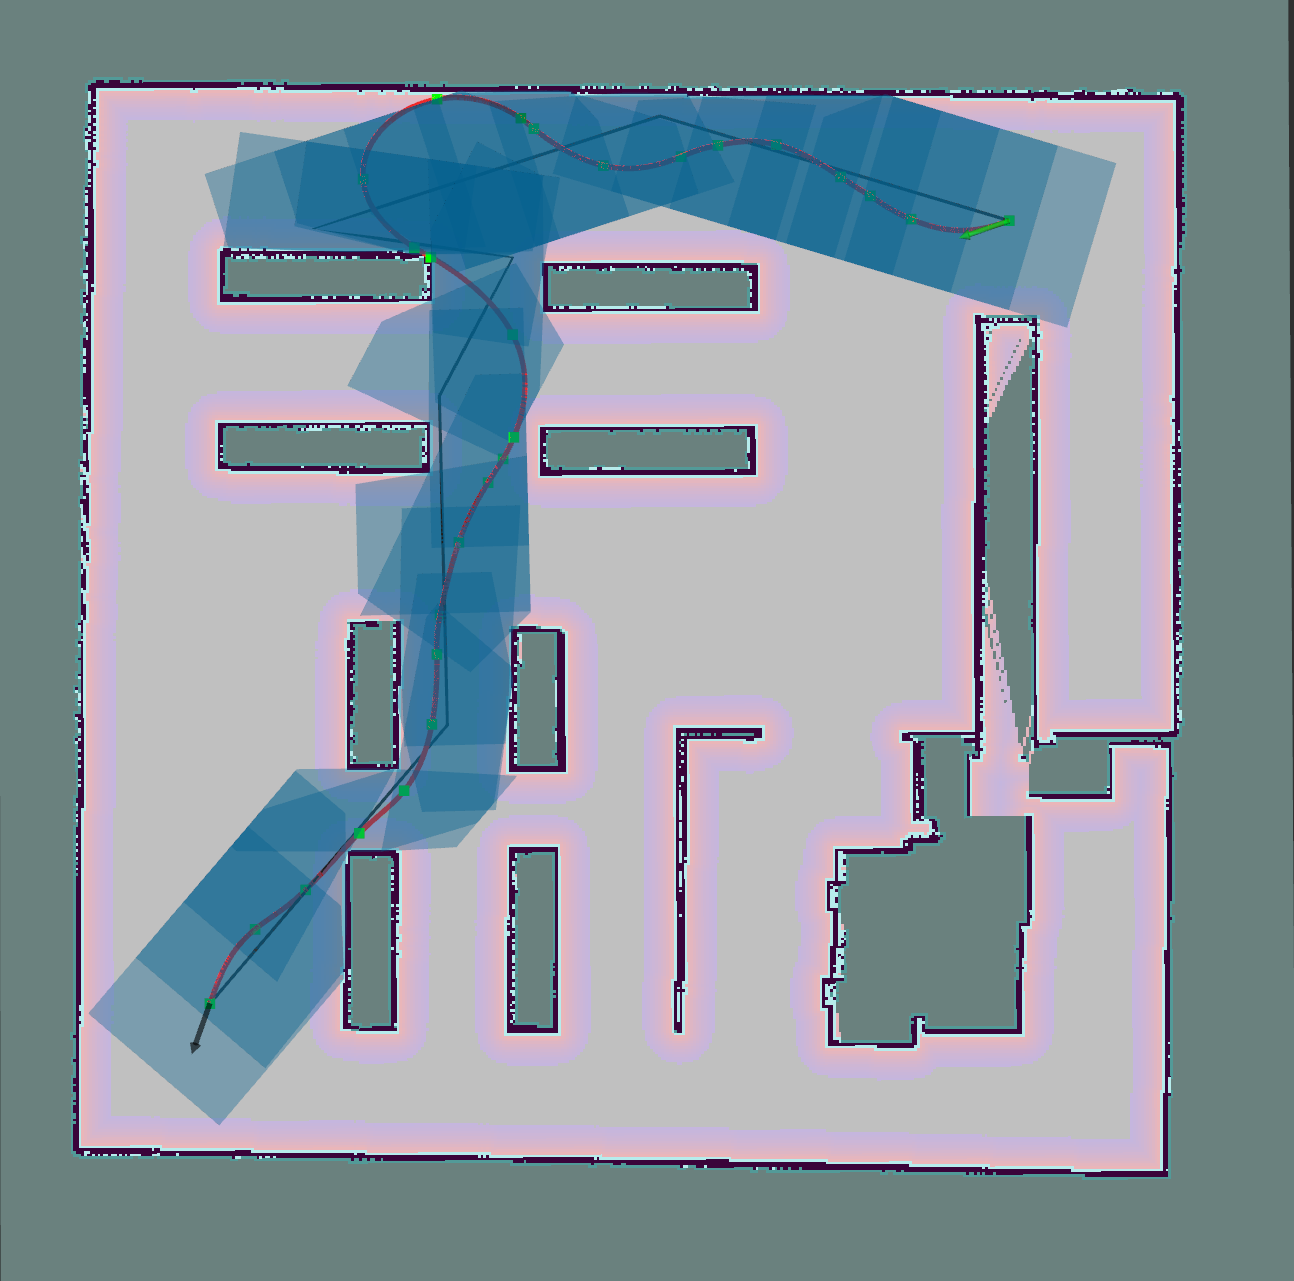
\includegraphics[width=0.4\textwidth]{single_3.png}}
			\subcaptionbox{示意二\label{fig:single_4}}[0.49\textwidth]{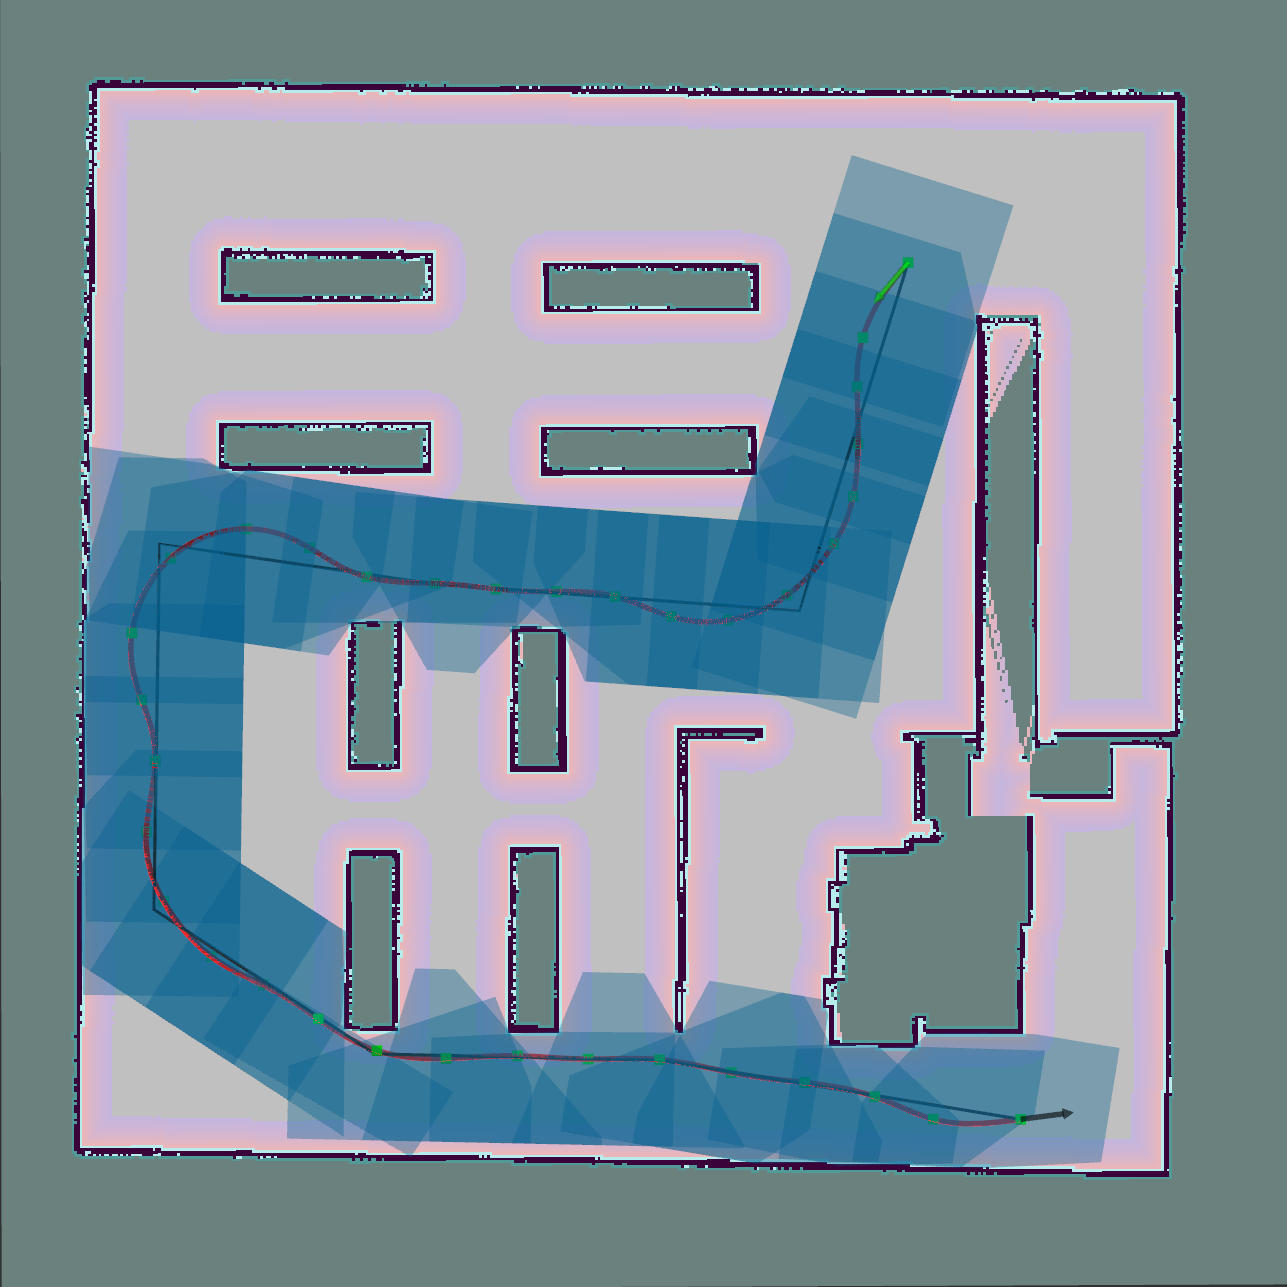
\includegraphics[width=0.4\textwidth]{single_4.png}}
			\caption{不同起点、终点下的路径规划仿真图}
			\label{fig:点到点路径规划仿真案例}
		\end{figure}

		\begin{figure}[H]
			\centering
			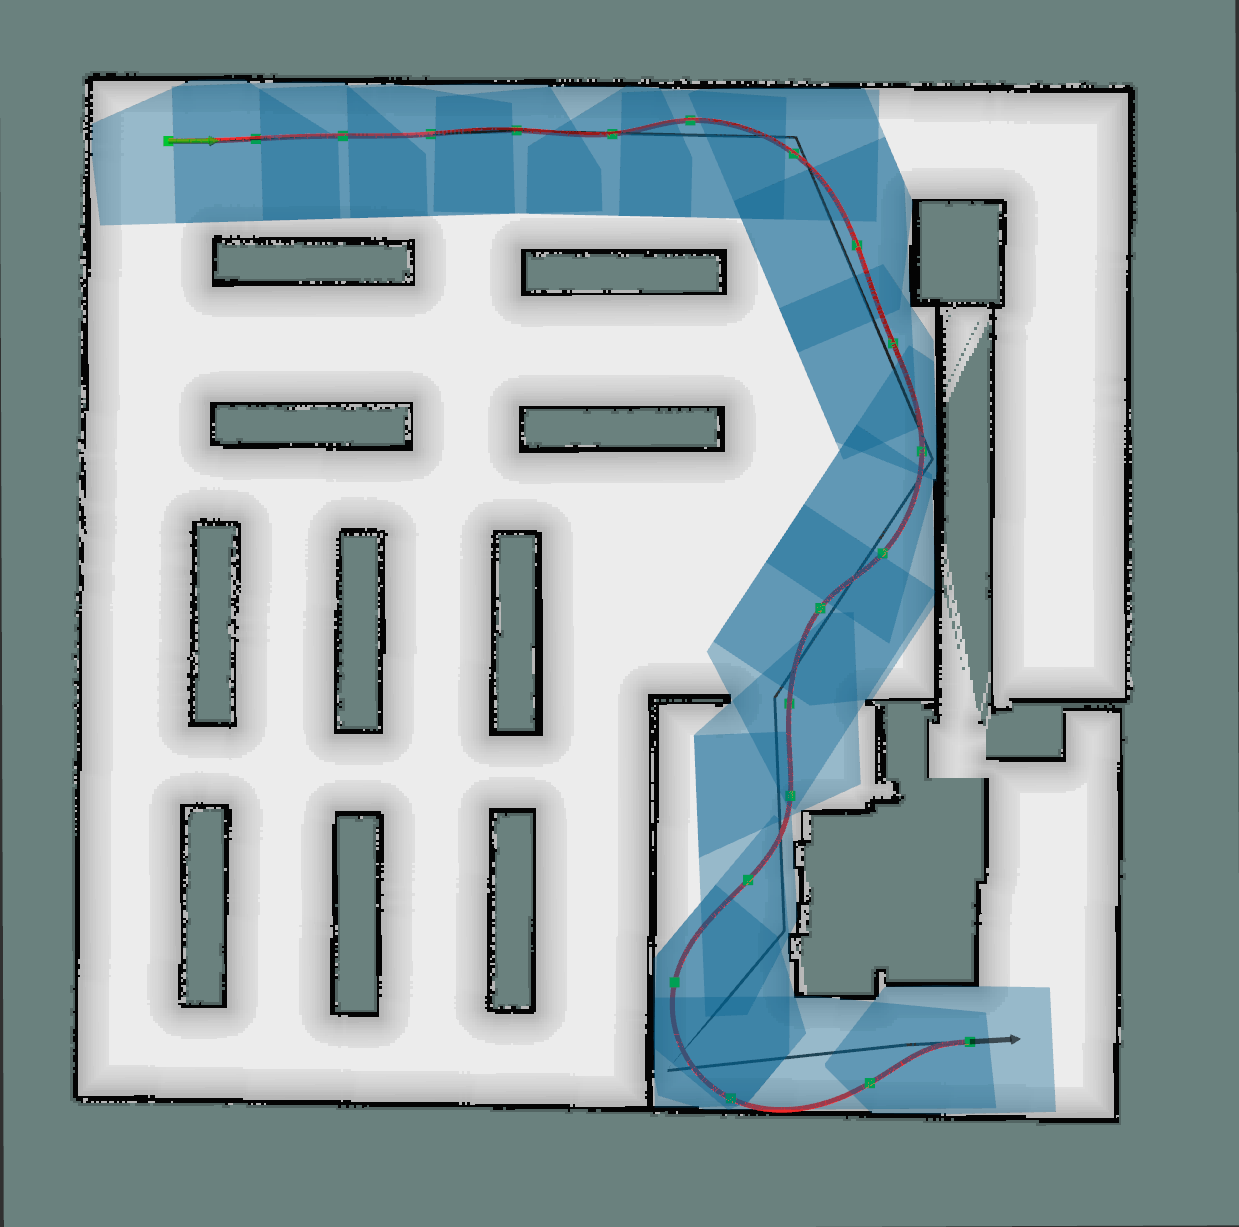
\includegraphics[width=0.7\textwidth]{single.png}
			\caption{障碍物场景及路径规划结果}
			\label{fig:single}
		\end{figure}
		
		在图 \ref{fig:点到点路径规划仿真案例}和\ref{fig:single} 中,黑色细线代表由RRT-Connect算法搜索出的初始路径,蓝色区域表示沿着该路径生成的安全走廊,而红色平滑曲线则展示了经优化算法处理后的最终路径。通过对比可以明显看出,优化后的轨迹不仅保证了足够的安全性和平滑度,而且其曲率(即转弯幅度)保持在一个合理的范围内。此外,起点和终点的方向与车体方向(如图中箭头所示)一致,进一步确保了路径的可用性。

		接下来,将简要分析图\ref{fig:single}对应的路径仿真数据。图 \ref{fig:datasingle} 展示了路径的曲率曲线,为了便于详细比较,重新绘制了优化后的全局轨迹。从右子图可以看出,在坐标点(80,0)附近,对应于路程160米处的曲率达到最大值0.097。整个曲率曲线的值始终小于0.1,这意味着曲率半径始终大于10米,这与仿真中设置的优化参数相吻合,证明了优化算法的有效性和合理性。

		\begin{figure}[H]
		\centering
		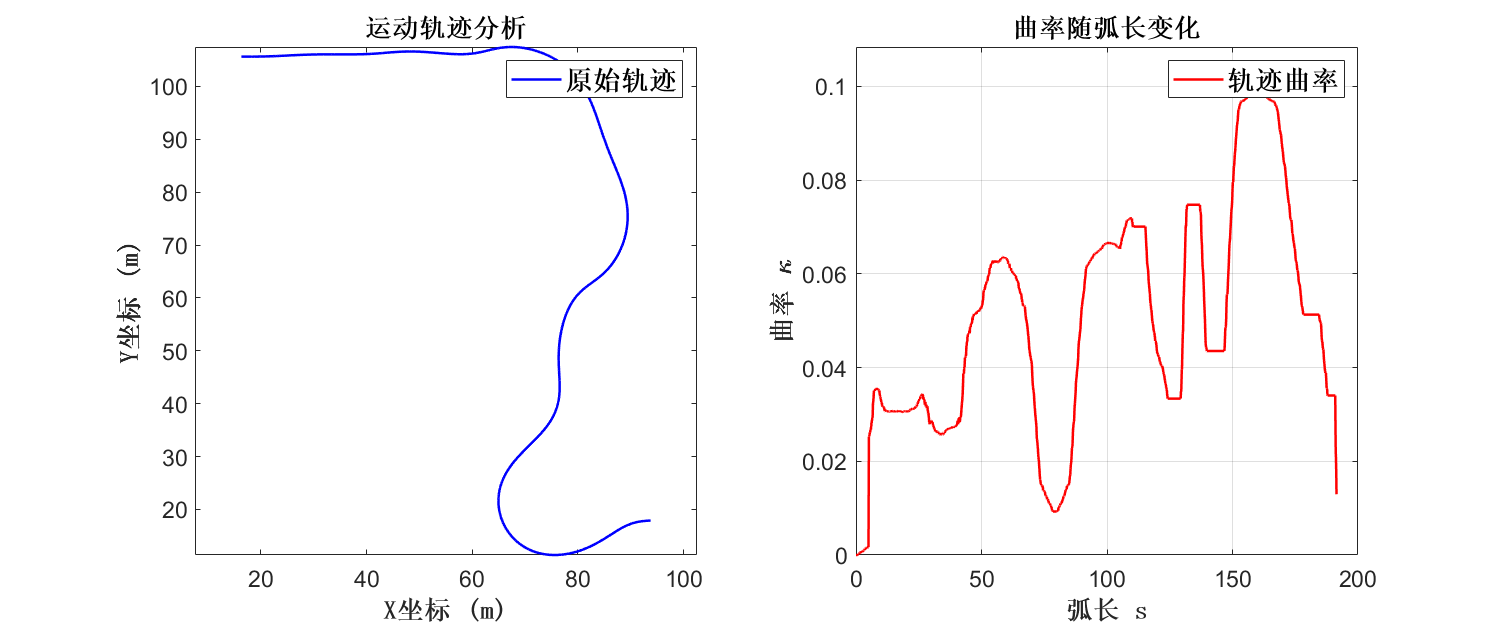
\includegraphics[width=1\textwidth]{datasingle.png}
		\caption{路径及其曲率分析}
		\label{fig:datasingle}
		\end{figure}

		本算法分为前端搜索和后端路径优化两大部分,各部分运行时间记录在表 \ref{tab:global_planning_time} 中。仿真结果显示,后端优化阶段在200米平均行程中的平均耗时为10.14毫秒,满足高实时性要求。前端RRT-Connect算法通过OMPL(Open Motion Planning Library)库实现,平均求解时间为6.07毫秒。整个算法总平均求解时间达17.71毫秒,性能表现优异。
		\begin{table}[!ht]
			\caption{全局规划算法求解耗时统计}
			\label{tab:global_planning_time}
			\centering
			\begin{tabular}{cccc}
				\toprule
				算法   & 最小值/ms & 最大值/ms & 平均值/ms \\
				\midrule
				前端搜索(RRT-Connect算法) & 3.04    & 12.22   & 6.07       \\
				路径优化       & 0.38    & 21.44    & 10.14      \\
				总耗时         & 4.32    & 24.18    & 17.71      \\
				\bottomrule
			\end{tabular}
		\end{table}

		综上,通过精心设计的障碍物场景测试、详尽的路径曲率分析以及算法运行时间评估,验证了所提出的路径规划方法在复杂环境中的高效性与可靠性,并证明其能满足实际应用中对安全性和实时性的严格要求。

		\subsection{多站点路径规划仿真}
		本节将介绍多站点路径规划算法的测试结果。在该场景下,每个站点均作为转向点,允许车辆在这些位置调整行驶方向。

		图 \ref{fig:多点路径规划仿真案例}展示了多站点路径规划的仿真案例。图\ref{fig:datamuti}展示了图\ref{fig:多点路径规划仿真案例}\subref{fig:muti}的轨迹和弧长变化曲线。测试中手动设置了6个航点,依次为A、B、C、D、E和F,其中A为起点,F为终点,其余四点(B、C、D、E)作为中间换向站点。蓝色区域表示安全走廊,红色曲线则为优化后的最终路径。每个站点处的两条路径切线方向保持一致,确保车辆可在此类关键点完成转向操作(例如从前进切换为倒车)。
		\begin{figure}[H]
			\centering
			\subcaptionbox{多站点路径规划\label{fig:muti}}[0.49\textwidth]{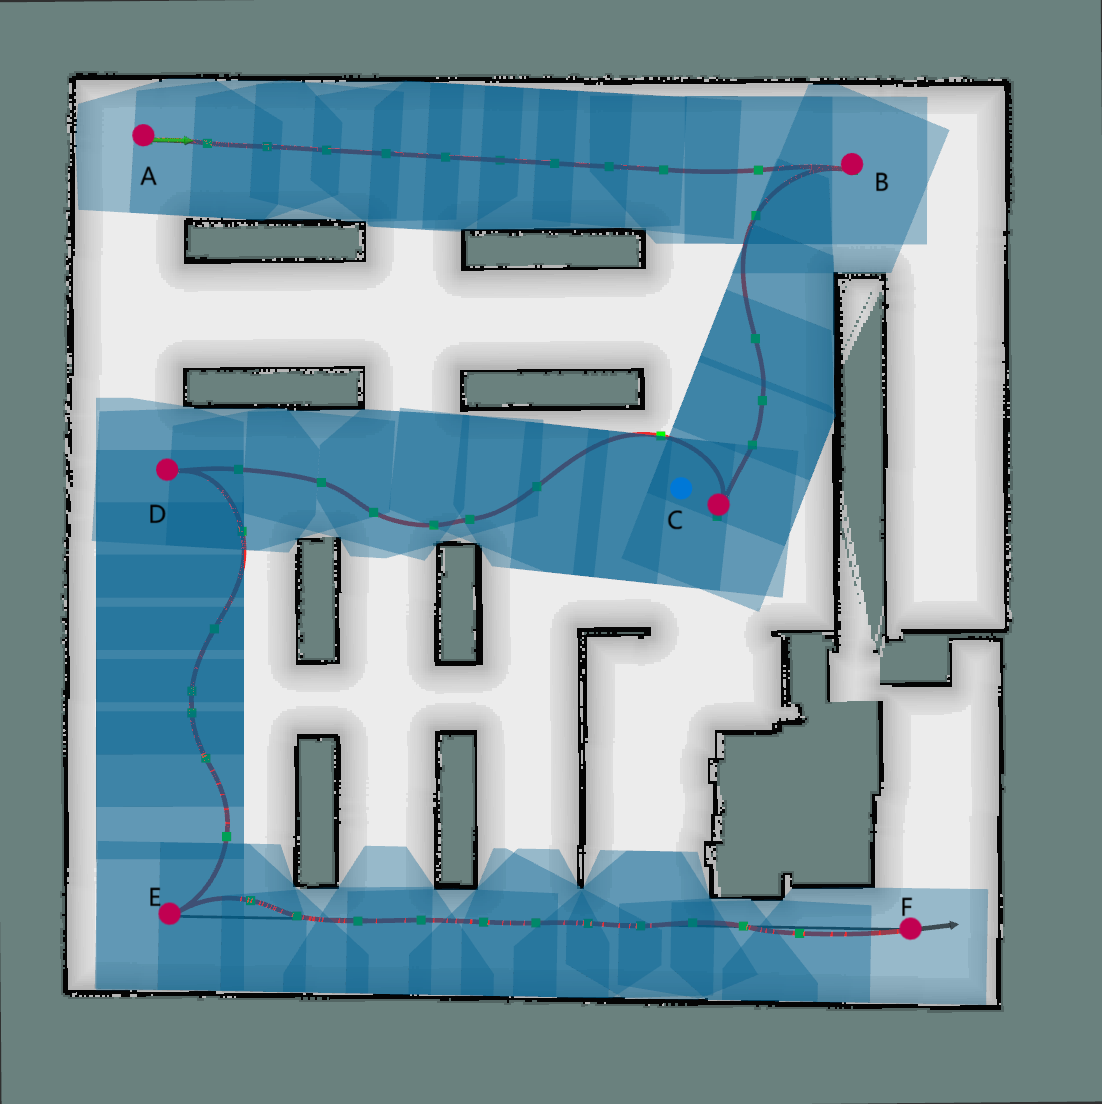
\includegraphics[width=0.344\textwidth]{muti.png}}
			\subcaptionbox{室内场景路径规划\label{fig:dataminco}}[0.49\textwidth]{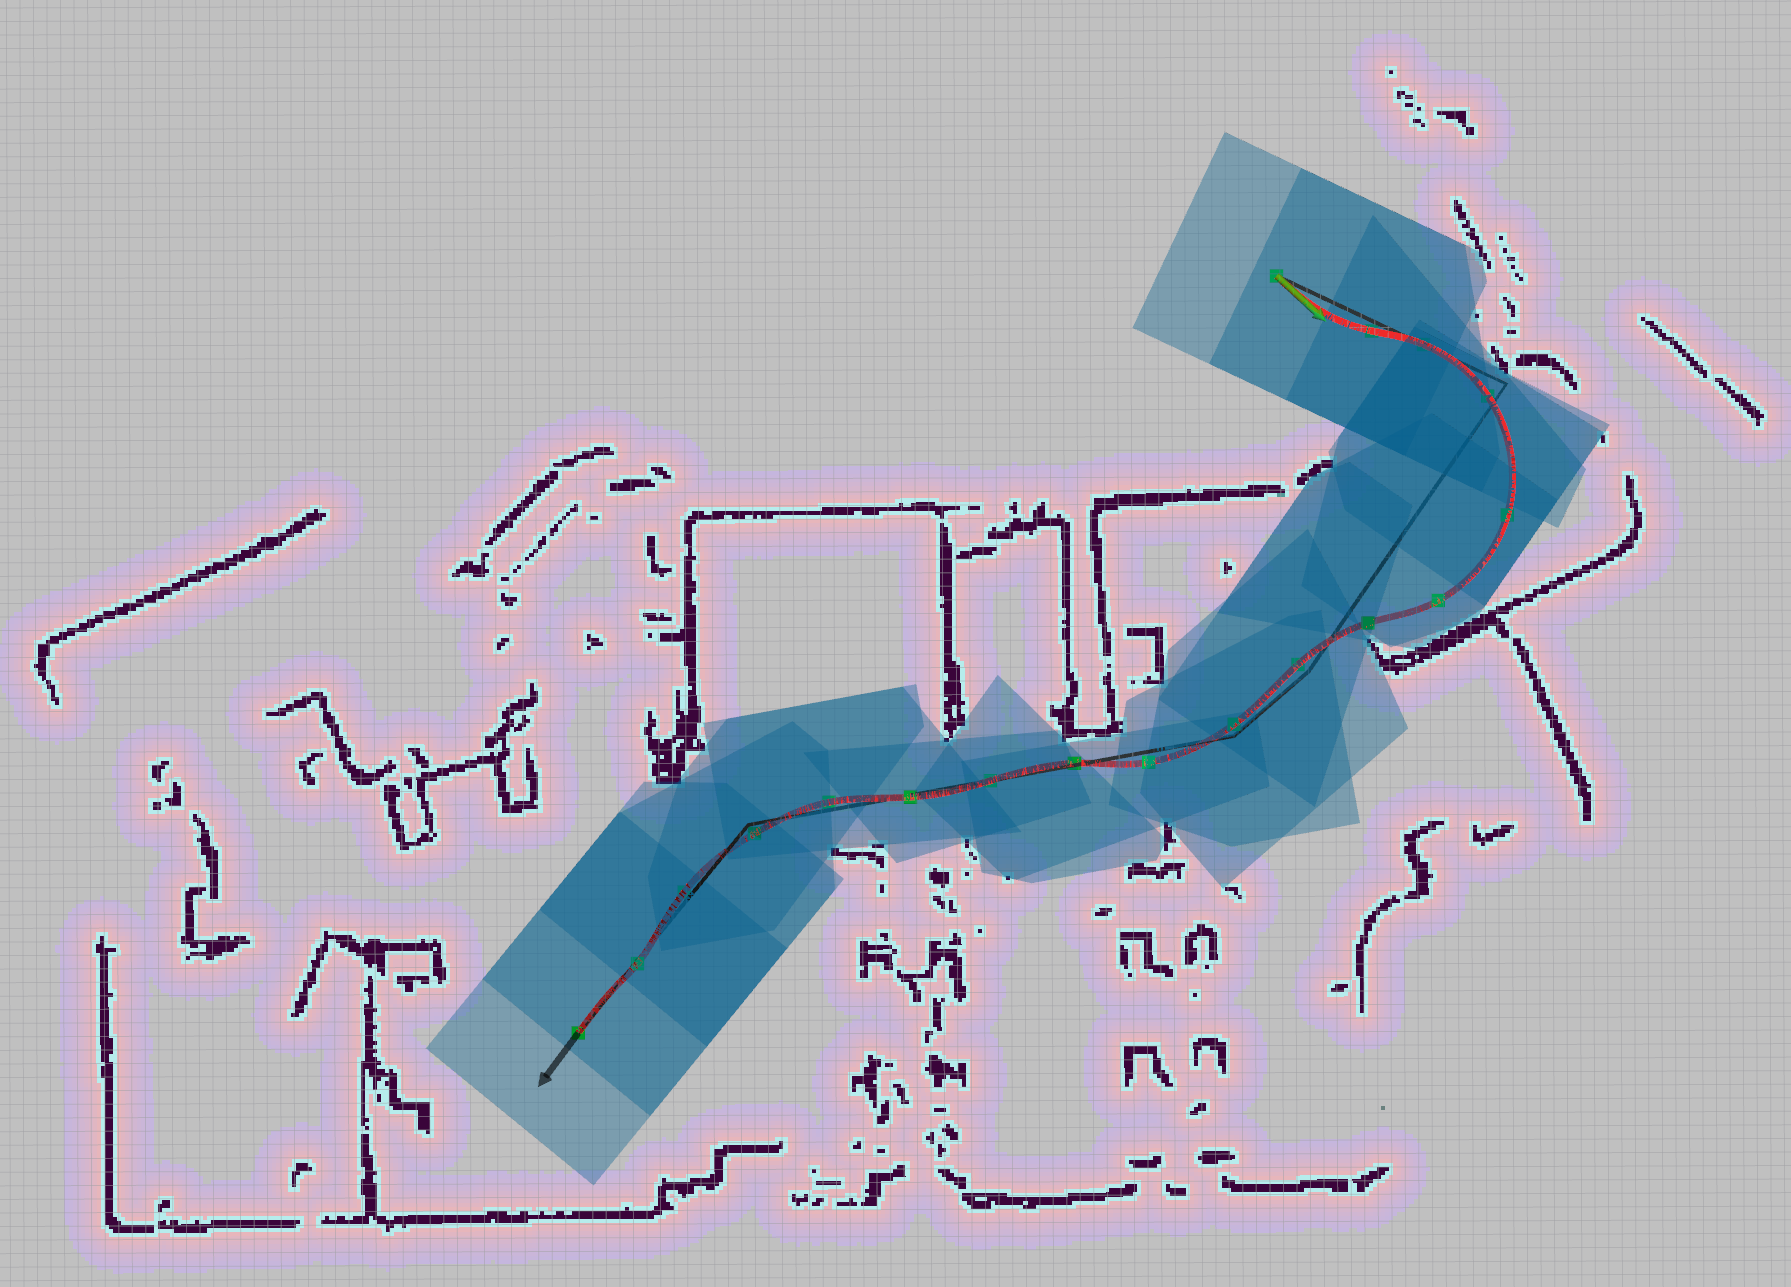
\includegraphics[width=0.48\textwidth]{dataminco.png}}
			\caption{多站点路径规划仿真案例}
			\label{fig:多点路径规划仿真案例}
			\end{figure}

			\begin{figure}[H]
				\centering
				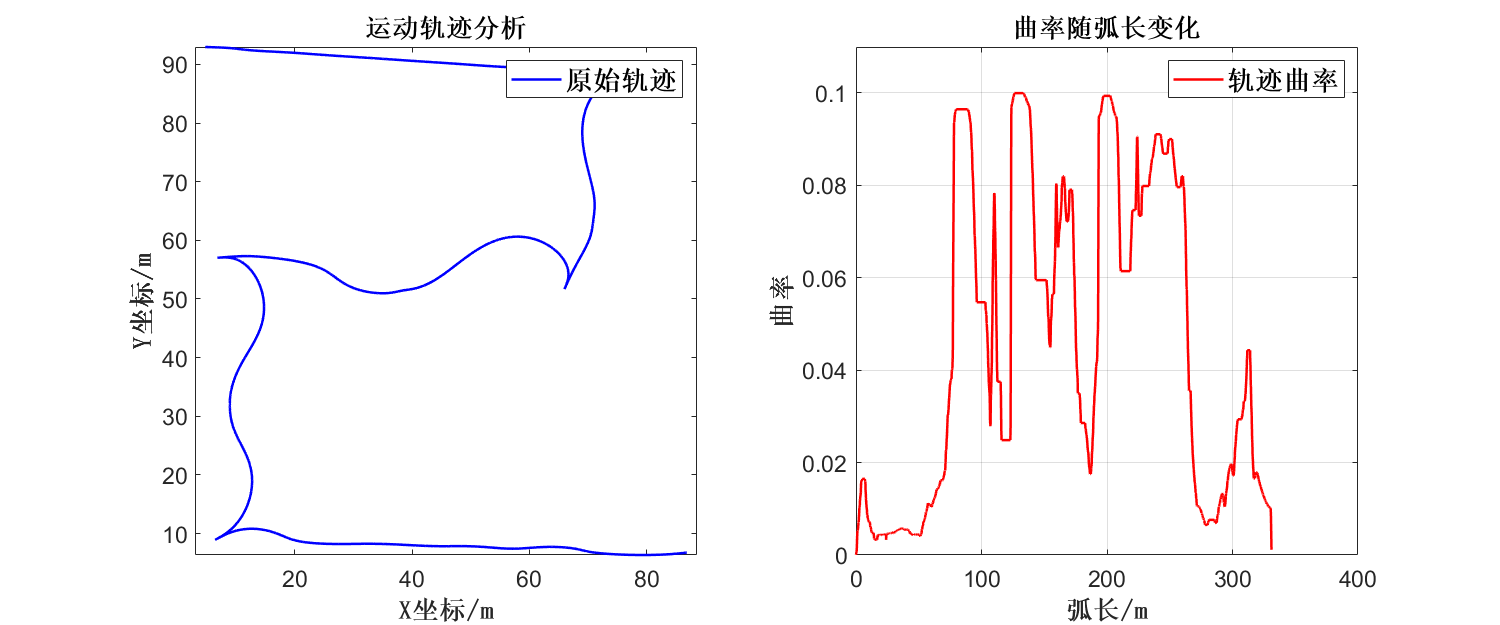
\includegraphics[width=1\textwidth]{datamuti.png}
				\caption{路径和的曲率变化曲线}
				\label{fig:datamuti}
				\end{figure}
		
			为了更深入地分析算法特性,下面对图\ref{fig:多点路径规划仿真案例}\subref{fig:muti}的仿真数据进行分析。图\ref{fig:datamuti}呈现了优化后全局轨迹的轨迹曲率随路程的变化情况。如图所示,在路程为80米、140米和210米处,曲率值接近预设的最大阈值0.1,但始终未超过该限值,从而保证了曲率半径始终大于10米。这一结果不仅符合优化参数的约束条件,也验证了算法在复杂场景下的稳定性和可靠性。

			通过本次多站点路径规划的仿真测试,不仅验证了算法在处理多个转向点时的有效性,还展现了其在路径平滑度与安全性保障方面的优异性能。结合详细的曲率分析,进一步验证了算法的稳定性,表明其能够满足实际应用中的工程约束要求。未来研究将聚焦于算法性能的进一步优化,并探索其在多样化复杂场景中的适用性。
		
	\section{局部规划算法仿真}
	在本节中,将对局部规划算法进行仿真测试,重点验证其避障能力。详细的算法理论部分已在第四章中进行了介绍。为了确保仿真的准确性和一致性,使用了通用的车体参数,具体参数值见表 \ref{tab:仿真车体参数}。此外,针对局部规划特有的参数提供了说明,详见表 \ref{tab:局部规划仿真参数}。
	\begin{table}[!ht]
		\caption{局部规划仿真参数}
		\label{tab:局部规划仿真参数}
		\centering
		\begin{tabular}{CLR}
			\toprule
			参数 & 描述 & 数值 \\
			\midrule
			$w_{u\omega}$ &铰接角速度代价惩罚权重 &1\\
			$w_{uj}$ &加加速度代价惩罚权重 &1\\
			$w_t$ &时间代价惩罚权重 &1\\
			$w_{kin}$ &运动学约束惩罚权重 &1000\\
			$w_{c}$ &走廊约束惩罚权重 &1000\\
			$w_{b}$ &优化变量边界约束惩罚权重 &1000\\
			\bottomrule
		\end{tabular}
	\end{table}
	从表 \ref{tab:局部规划仿真参数} 中可以看出,本文在铰接角速度代价、加加速度(舒适度)代价及时间最优代价上设置了相对较小的权重。这主要是因为本文提出的算法本质上是一个运动规划算法,允许对输入量进行适度松弛且不苛求严格时间最优性。而对于需严格满足的三类约束——运动学约束(平滑性)、走廊约束(安全性)与边界约束(可行性),均设定了1000量级的高权重配置。

	为了展示局部规划算法的效果,本文在仿真环境中设置了多种障碍物配置,并记录了算法在不同场景下的表现。如图 \ref{fig:局部规划仿真案例} 所示,展示了局部规划算法在不同场景下的仿真结果。这些场景包括泊车、穿越狭窄区域以及绕过障碍物等典型情况。在图 \ref{fig:局部规划仿真案例}\subref{fig:s1}、\ref{fig:局部规划仿真案例}\subref{fig:s2} 和 \ref{fig:局部规划仿真案例}\subref{fig:s3} 中,蓝色线条代表由算法生成的最终轨迹,浅蓝色区域表示安全走廊。
	\begin{figure}[H]
		\centering
		\subcaptionbox{泊车场景\label{fig:s1}}[0.49\textwidth]{\includegraphics[width=0.4\textwidth]{s1.png}}
		\subcaptionbox{狭窄场景\label{fig:s2}}[0.49\textwidth]{\includegraphics[width=0.4\textwidth]{s2.png}}
		\subcaptionbox{狭窄空间中的安全走廊\label{fig:s3}}[0.49\textwidth]{\includegraphics[width=0.4\textwidth]{s3.png}}
		\subcaptionbox{绕障场景\label{fig:s4}}[0.49\textwidth]{\includegraphics[width=0.4\textwidth]{s4.png}}
		\caption{局部规划算法在部分场景中的规划结果展示}
		\label{fig:局部规划仿真案例}
	\end{figure}

	进一步,在图 \ref{fig:局部规划仿真案例}\subref{fig:s4} 中,紫色线条表示由Hybrid A*算法生成的初始解,绿色线条是本文算法输出的最终轨迹。明显看出,优化后的轨迹拐点较少,具有更少的换向次数,这不仅提高了路径的平滑度,还增强了车辆行驶的舒适性和安全性。

	图 \ref{fig:nmpcyuewa1}展示了穿越室内场景的仿真结果。其中,蓝色细线表示Hybrid A*算法生成的初始路径,而粗线则对应优化处理后的最终轨迹。优化后的路径在平滑性、避障能力和路径长度方面均有显著提升。下面两小节将主要对自主泊车场景和侧方位停车场景进行详细的仿真分析。

	\begin{figure}[H]
		\centering
		\includegraphics[width=0.7\textwidth]{nmpcyuewa1.png}
		\caption{室内栅格地图规划结果展示}
		\label{fig:nmpcyuewa1}
	\end{figure}

		\subsection{自主泊车场景}
		在自主泊车场景中,算法需同时支持前进与后退两种运动模式,然而许多现有规划算法(如五次多项式)并未明确区分这两种模式。相比之下,本文提出的算法基于精确的运动学模型构建,能够自然切换前进与后退模式。图 \ref{fig:boche} 为泊车场景中Hybrid A*算法与优化后路径的对比仿真结果。
		\begin{figure}[H]
			\centering
			\includegraphics[width=0.6\textwidth]{boche.png}
			\caption{Hybrid A*算法与优化后的轨迹对比}
			\label{fig:boche}
		\end{figure}
		
		图中,铰接车以绿色箭头位置为起始点,并最终停驻于灰色箭头指示的目标位置。深蓝色细线表示改进版Hybrid A*算法生成的轨迹,该轨迹在接近终点时需完成三次转向才能完成泊车任务。为确保安全,基于Hybrid A*轨迹构建了膨胀后的安全走廊。只要铰接车始终位于该安全区域内,即可有效避免碰撞。可以看出,局部规划算法生成了更流畅的绿色轨迹,其在接近终点时仅需一次转向即可完成泊车任务。尽管局部规划算法以Hybrid A*生成的路径作为初始路径,但最终轨迹质量显著优于前者,换向次数大幅减少。这表明,即使初始路径质量欠佳,本文提出的算法仍可通过迭代优化将轨迹优化至较高水平,且表现出较低的初值敏感度。


		接下来,本文将对仿真数据进行详细分析,以进一步评估算法性能。图 \ref{fig:databochestate}展示了图\ref{fig:boche}中轨迹的航向角、铰接角、车辆速度及加速度随时间的变化曲线。
		\begin{figure}[H]
			\centering
			\includegraphics[width=1\textwidth]{databochestate.png}
			\caption{泊车轨迹状态变量曲线}
			\label{fig:databochestate}
		\end{figure}

		如图所示,航向角与车速曲线呈现连续且平滑的特性,这主要得益于精确运动学模型的采用。这种平滑性对保障车辆行驶过程中的稳定性和安全性至关重要。其次,车体速度在整个过程中保持在-1 m/s至3 m/s的范围内,而加速度则在-0.4 m/s$^\text{2}$至0.4 m/$s^\text{2}$之间波动,均符合表\ref{tab:仿真车体参数}设计要求。然而,铰接角与加速度曲线虽保持连续性,但其斜率偶尔出现小幅度突变。其原因在于铰接角与加速度分别与输入量(铰接角速度与加加速度)之间仅存在一阶导数关系。由于控制输入可为不连续信号,导致铰接角与加速度无法保证全程可微性。尽管如此,此类现象对车辆整体性能影响有限,因铰接角始终控制在-0.5 rad至0.5 rad的安全范围内,满足操作需求。值得注意的是,在0秒至26秒期间,铰接车速度为正值,表明车辆处于前进状态。至26秒时,车速降至0 m/s,标志着车辆抵达转向点。此时结合示意图 \ref{fig:boche} 可见,铰接角同步归零(0 rad),表明铰接结构完全回正。随后,车速转为负值,车辆开始倒车并成功泊入目标区域。
		
		图\ref{fig:databocheinput}展示了优化轨迹的输入量变化曲线。从图中可见,在5秒、17秒和24秒时刻,加加速度(jerk)发生突变,对应的角速度曲线也出现相应突变。
		\begin{figure}[H]
			\centering
			\includegraphics[width=1\textwidth]{databocheinput.png}
			\caption{泊车轨迹输入变量曲线}
			\label{fig:databocheinput}
		\end{figure}
		
		这一现象源于系统输入量未受微分方程约束,允许非连续变化。然而,输入变量由于受到边界约束,始终与预设的边界约束条件保持一致:铰接角速度严格限制在-0.2 rad/s至0.2 rad/s之间,加加速度则控制在-0.3 m/s$^\text{3}$至0.3 m/s$^\text{3}$之间。
		

		表\ref{tab:local_planning_boche_time}是局部规划算法的平均求解耗时统计,每个场景测试了20次。
		\begin{table}[!ht]
			\caption{局部规划算法求解耗时统计}
			\label{tab:local_planning_boche_time}
			\centering
			\begin{tabular}{l rrr}
				\toprule
				场景   &  路径长度/m & 求解耗时/ms \\
				\midrule
				避障场景1 & 25    & 78.2   \\
				避障场景2 & 35    & 106.0  \\
				避障场景3 & 45    & 147.8  \\
				泊车场景1  & 35   & 207.4  \\
				泊车场景2  & 45   & 515.2  \\
				\bottomrule
			\end{tabular}
		\end{table}

		\subsection{侧方位停车场景}
		侧方位停车与自主泊车具有同等重要性,本小节将对侧方位停车场景开展仿真测试。图\ref{fig:cebianboche}为侧方位泊车的RVIZ可视化仿真结果,图\ref{fig:datacebianstate}则展示了对应的车辆状态数据曲线。细线轨迹由改进的Hybrid A*算法生成,在接近终点时通过一次转向操作完成泊车任务。粗线轨迹为局部规划算法优化后的最终路径,呈现S形特征。其轨迹平滑性显著优于改进的Hybrid A*算法生成的轨迹,同时在侧方位停车场景中未发生转向操作,并且路径长度明显更短。
		\begin{figure}[H]
			\centering
			\includegraphics[width=0.65\textwidth]{cebianboche.png}
			\caption{侧边泊车场景}
			\label{fig:cebianboche}
		\end{figure}

		% 图\ref{fig:datacebianstate}是侧边泊车的状态曲线图,包括航向角、铰接角、速度和加速度。可以从速度曲线看出,由于并没有发生换向,所以铰接车的速度始终保持为正。
		\begin{figure}[H]
			\centering
			\includegraphics[width=1\textwidth]{datacebianstate.png}
			\caption{侧边泊车状态变量曲线}
			\label{fig:datacebianstate}
		\end{figure}

		图\ref{fig:datacebianstate}展示了侧方位泊车场景下的时序数据,涵盖航向角、铰接角、车辆速度及加速度曲线。铰接角曲线显示,在S形轨迹的前半段,铰接角为负值(<0 rad),表明车辆向右转向;后半段铰接角转为正值(>0 rad),表明车辆向左转向,最终在终点处铰接角归零(0 rad),车体完全回正。速度曲线表明,由于泊车过程中未发生转向操作,铰接车在整个过程中保持正向行驶状态,车速始终维持正值。

		\subsection{局部规划算法的性能对比}
		为了全面地评估本研究提出的局部轨迹规划算法性能,本文将其与文献\cite{9216948}中提出的算法进行了对比分析。为简化叙述过程,本文将该参考文献中的算法称为OBPP算法(Optimization Based Path Planning)。图\ref{fig:Hybrid A*、OBPP算法、本文的局部规划算法对比图}展示了不同算法(Hybrid A*、OBPP算法以及本文提出的局部规划算法)的规划结果。OBPP算法通过构建基于最优控制的规划问题,并采用增广拉格朗日方法处理约束条件。尽管该方法在轨迹优化中表现出有效性,但其引入的大量协态变量显著增加了计算成本。此外,其避障策略依赖于自车结构与障碍物凸包的距离计算,导致环境中障碍物数量的增加会直接引发约束条件的线性增长。
		\begin{figure}[H]
			\centering
			\subcaptionbox{对比图1\label{fig:局部对比1}}[0.49\textwidth]{\includegraphics[width=0.4\textwidth]{fig/局部对比1.png}}
			\subcaptionbox{对比图2\label{fig:局部对比2}}[0.49\textwidth]{\includegraphics[width=0.4\textwidth]{fig/局部对比2.png}}
			\subcaptionbox{对比图3\label{fig:局部对比3}}[0.49\textwidth]{\includegraphics[width=0.4\textwidth]{fig/局部对比3.png}}
			\subcaptionbox{对比图4\label{fig:局部对比4}}[0.49\textwidth]{\includegraphics[width=0.4\textwidth]{fig/局部对比4.png}}
			\caption{Hybrid A*、OBPP算法、本文的局部规划算法对比图}
			\label{fig:Hybrid A*、OBPP算法、本文的局部规划算法对比图}
		\end{figure}

		为确保对比结果的公平性与结果的可靠性,本文在实现过程中采用IPOPT(Interior Point OPTimizer)求解器对提出的局部规划算法及OBPP算法进行数值求解,并借助CasADi自动微分工具完成梯度计算。两种算法的初始粗略路径均基于Hybrid A*算法生成。

		图\ref{fig:Hybrid A*、OBPP算法、本文的局部规划算法对比图}中,紫色轨迹对应Hybrid A*算法的输出,橙色轨迹为OBPP算法的规划结果,绿色轨迹则为本文提出的局部规划算法的优化路径。从图中可观察到,相较于OBPP算法生成的激进型轨迹,本文算法在转向点处展现出更高的轨迹平滑性,其运动轨迹更符合驾驶舒适性需求。

		表\ref{tab:局部仿真结果对比}比较了OBPP算法与本文算法在20米至30米路径长度范围内的表现,随机起点、终点共测试了40次,测试指标包括规划成功率、平均换向次数、舒适度以及算法求解耗时。平均舒适度的计算公式如下:
		\begin{equation}
			\begin{aligned}
				Comfort = \frac{\sum_{i=1}^{N}\Delta t_i}{\sum_{i=1}^{N}jerk_i*\Delta t_i} 
			\end{aligned}
		\end{equation}
		其中,$jerk_i$为第$i$步系统的输入变量,参考第四章。$\Delta t_i$为第$i$步系统的离散时间。

		\begin{table}[!ht]
			\caption{20米至30米路径长度时几种算法的性能对比}
			\label{tab:局部仿真结果对比}
			\centering
			\begin{tabular}{CCCCC}
				\toprule
				算法 & 成功率 &平均换向次数/times &舒适度/[s$^{3}$/m] &求解耗时/ms\\
				\midrule 
				本文局部规划算法 &100\% &1.2 &16.13 &79.3\\
				OBPP &87.4\% &1.2 &14.08 &21817.1 \\
				\bottomrule
			\end{tabular}
		\end{table}
		
		数据显示,本文提出的算法不仅拥有更高的成功率,而且求解耗时也远低于OBPP算法。原因在于OBPP算法在应对运动学约束、安全约束及时间约束时采用了增广拉格朗日方法,导致大量协态变量的引入,引发了维度爆炸的问题,增加了求解难度和失败风险。相反,本文的方法通过罚函数和微分同胚策略处理约束条件,避免了额外协态变量的引入,从而提高了计算效率和稳定性。

	\section{本章小结}
	在本章中,首先基于ROS(Robot Operating System)与RVIZ(RVIZ Visualization Toolkit)构建了仿真环境,并设计了面向运动规划的软件架构,旨在提升系统实时性与计算效率。随后,针对第三章提出的全局轨迹规划算法与第四章设计的局部轨迹规划算法,本文设计并实施了多组对比实验,以全面验证算法在复杂场景下的有效性与工程实用性。通过系统仿真,不仅验证了算法在动态障碍物密集场景中的轨迹优化能力,还进一步验证了其实时性与鲁棒性等工程指标,为算法的实际应用提供了可靠的技术支撑。

	\chapter{结论}
	本文将铰接车的轨迹规划任务分解为全局规划和局部规划两个阶段,并分别进行了算法设计,全文工作总结如下:

	(1)建立了铰接式车辆的无滑移运动学模型,基于最优控制理论对轨迹规划问题进行数学建模。

	(2)针对铰接车全局轨迹规划,本文提出了一种基于微分平坦理论与Minco样条的全局轨迹规划算法。通过选取笛卡尔坐标系作为平坦输出,将非完整约束转化为平坦空间中的代数关系,并采用Minco样条对轨迹进行参数化建模。通过构建包含起点状态、终点状态、中间航点位置及高阶导数连续性的边界值问题(BIVP)约束体系,给出基于航点向量的闭式解形式。针对避障需求,设计了安全走廊算法,利用凸多边形约束实现障碍物规避;同时引入曲率约束松弛函数,将铰接角硬约束及走廊安全约束转换为代价函数项,通过L-BFGS算法实现高效求解。

	(3)针对局部轨迹规划,本文提出了一种基于安全走廊的时空联合轨迹规划方法。 首先,对铰接车进行几何建模,将其表示为连接两个矩形的刚体模型,将避障问题转化为多边形几何碰撞检测问题。其次,改进Hybrid A*算法以适应铰接车运动学特性:通过调整节点拓展策略并结合运动学约束,提升路径规划效率与准确性;同时设计了基于栅格地图与Bresenham算法的碰撞检测模块,实现障碍物的高效检测。在轨迹优化阶段,构建了基于NMPC的规划框架,引入动力学约束、运动学约束及避障约束,并通过外罚函数与微分同胚方法将约束条件消去,最终实现无约束高效求解。

	(4)设计了仿真验证了全局规划和局部规划算法的有效性和鲁棒性。通过在点到点导航场景和多点导航场景下进行全局规划测试,验证了全局规划算法在复杂环境中的可靠性。同时,通过在自主泊车场景和侧方位停车场景下进行局部规划测试,验证了局部规划算法的避障能力。

	综上所述,本文所提出的基于全局规划和局部规划的铰接车轨迹规划方法能够有效解决铰接车在复杂非结构化环境中的轨迹规划问题,有助于提高铰接车整体自主化的水平。

	本文提出的解决方案虽然能够在复杂环境中实现铰接车的轨迹规划,但仍存在一些不足之处,有待进一步改进和完善:

	(1)由于实验条件的限制,算法尚未应用于真实的铰接式车辆上,因此无法充分评估其在不确定环境下的鲁棒性。未来的研究应致力于将算法部署到实际车辆中,以验证其在真实世界中的性能表现。

	(2)本文提出的全局规划基于样条曲线,使用采样的方式施加曲率约束,在采样点处严格满足曲率约束。但多次仿真发现尽管采样点足够密集,但采样点之间仍然可能会出现曲率骤变的情况,尤其是在航点附近。针对这个问题,未来将致力于在连续域上施加曲率约束。

	尽管本文提出的解决方案在复杂环境中的铰接车路径规划方面取得了一定进展,但在实际应用、实时性和鲁棒性等方面仍需进一步优化和改进。未来的研究将继续致力于这些方面的提升,以期实现更高效、更可靠的路径规划系统。
																					  
	\reference{ref.bib}

	% \customizedappendix{
	% }

	% \customizedappendix{
	% }

	\achievement{
		{\vspace{-0.1em}\noindent\textbf{\songtib\zihao{-4} 1.\enspace 发表的学术论文}\vspace{-0.41em}}    % 无学术论文时此项不必列出
		\begin{enumerate}[leftmargin=1.52em,itemsep=-0.4em,label={[\arabic*]}]\zihao{5}%%%%%%% 这一行的设定不要修改!!!
			\item YANG Y, LUO X, CHEN K, et al. A spatial-temporal trajectory planner for center-articulated vehicles[C]//2024 4th International Conference on Artificial Intelligence, Robotics, and Communication (ICAIRC). IEEE,2024: 442-448. (国际会议论文,EI收录号:20251318118964)
		\end{enumerate}
	}

	\acknowledgement{
		时光荏苒,如白驹过隙,三年研究生生涯转瞬即逝。值此论文完稿之际,谨向所有给予我支持与帮助的师长亲友表达最诚挚的谢意。

		首先,我要特别感谢我的导师华长春教授和骆曦老师。三年来,您们以渊博的学识、严谨的治学态度和饱满的科研热忱为我树立了学术标杆。无论是论文选题的反复推敲,还是研究瓶颈期的耐心指导,您们的谆谆教诲始终是我学术道路上的明灯。

		在课题研究过程中,HCC课题室的同门给予了我全方位的支持:特别感谢穆殿瑞、陈健楠两位师兄在论文框架与格式规范上的专业指导;朱百强伙计与我日夜相伴探讨思路,彼此的灵感碰撞让枯燥的科研充满火花;陈阔、卢方耀两位伙伴逐字推敲语言表达,耿波、莫亿龙、马长乐、刘畅等战友与我共同攻克实验难题。特别感谢室友杨鹏飞在论文攻坚阶段提供的宝贵建议,这份同窗情谊将永远珍藏。

		最后,我要向七年来坚持"一路向北"的自己致敬。从本科到硕士的时光淬炼,那些在实验室通宵达旦的夜晚,那些被数据困扰却依然执着的清晨,终将化为通向未来的基石。站在新的人生起点,惟愿不负韶华,继续追寻真理之光

	}
\end{document}
